\documentclass[runningheads]{jblab}

\usepackage[utf8]{inputenc}
\usepackage[english,russian]{babel}
\usepackage[T2A]{fontenc}
\usepackage{amsmath}
\usepackage{tikz}
\usetikzlibrary{arrows}
\usepackage{indentfirst}
\usepackage{amsfonts}
\usepackage{amssymb}
\usepackage{graphicx}
\usepackage{listings}
\usepackage{algpseudocode}
\usepackage{algorithm}
\usepackage{caption}
\usepackage{algorithmicx}
\usepackage{wrapfig}
\usepackage{supertabular}
\usepackage{epigraph}
\usepackage{euscript}
\usepackage{textcomp}
\usepackage{cite}
\usepackage{ucs}
\usepackage[caption=false]{subfig}

\usepackage{xcolor}
\definecolor{dkgreen}{rgb}{0,0.6,0}
\definecolor{dred}{rgb}{0.545,0,0}
\definecolor{dblue}{rgb}{0,0,0.545}
\definecolor{lgrey}{rgb}{0.9,0.9,0.9}
\definecolor{gray}{rgb}{0.4,0.4,0.4}
\definecolor{darkblue}{rgb}{0.0,0.0,0.6}

\newcommand{\cd}[1]{\texttt{#1}}

\pdfpagewidth=14.8cm
\pdfpageheight=21cm

\textwidth=10cm
\textheight=15cm

\oddsidemargin=0pt
\evensidemargin=0pt

\topmargin=0pt

\makeatletter
\newcommand{\StatexIndent}[1][3]{%
  \setlength\@tempdima{\algorithmicindent}%
  \Statex\hskip\dimexpr#1\@tempdima\relax}
\algdef{S}[IF]{IfNoDo}[1]{\algorithmicif\ #1}%
\makeatother

\begin{document}

\newcommand{\Issue}[0]{2}
\newcommand{\Year}[0]{2014}
\sloppy

\begin{titlepage}

\centering


\includegraphics[width=4cm]{JBLogoWhite.png}
\vskip 2cm
\mbox{\Large{\textsc{Труды лаборатории}}}
\vskip 0.5cm
\mbox{\Large{\textsc{языковых инструментов}}}
%\vskip 0.5cm
%<\mbox{\Large{\textsc{компании JetBrains}}}
\vskip 2.5cm
\large{Выпуск \Issue}
\vskip 6cm
\large{Санкт-Петербург, \Year}
\end{titlepage}

\thispagestyle{empty}
\phantom{xx}
\pagebreak

\chapter*{Предисловие}

В октябре 2012 года компания JetBrains --- один из мировых лидеров в области 
производства средств поддержки разработки ПО --- анонсировала создание на
математико-механическом факультете Санкт-Петербургского государственного университета
лаборатории языковых инструментов. Задачей этой лаборатории является реализация
силами студентов и аспирантов факультета научно-исследовательских и образовательных 
проектов в областях компетенции компании.

Настоящий сборник представляет работы, выполненные студентами лаборатории в 2012-2013 учебном году.
Среди тем этих работ можно найти как классические, такие как управление памятью и сборка 
мусора, декомпиляция, форматирование исходных текстов, так и сравнительно 
новые направления, связанные с сертификационным программированием и анализом 
встроенных языков.

Следует отметить, что все представленные работы были не только проведены в лаборатории 
под руководством специалистов JetBrains, но и засчитаны их авторам 
в качестве курсовых или дипломных работ. 
\vskip 2cm
\begin{flushright}
\textit{куратор лаборатории Д.Булычев}
\end{flushright}

\tableofcontents

\title{Сборщик мусора\\
для языка Objective Caml\\
в инфраструктуре LLVM}
%
\titlerunning{Сборщик мусора для языка Objective Caml}
\author{Шашкова Елизавета Михайловна}
%
\authorrunning{Е.М.Шашкова} % abbreviated author list (for running head)
%
%%%% list of authors for the TOC (use if author list has to be modified)
\tocauthor{Е.М.Шашкова}
%
\institute{Санкт-Петербургский государственный университет\\
\email{Elizabeth.Shashkova@gmail.com}}

\maketitle              % typeset the title of the contribution

\section*{Введение}

Сборка мусора --- одна из форм автоматического управления памятью. Специальный компонент поддержки среды времени исполнения, 
называемый сборщиком мусора, автоматически освобождает 
память, удаляя объекты, которые больше не являются доступными для использования.  Сборка мусора освобождает программиста от 
необходимости вручную выделять и освобождать память и позволяет сконцентрироваться на выполнении других задач.
В большинстве современных языков все чаще происходит отказ от предоставления явных средств управления памятью в пользу сборки мусора.

Сборка мусора тесно связана с реализацией компилятора: например, он должен предоставлять сборщику мусора способ определить адреса корневых объектов во
время исполнения. Один из основных
подходов к созданию компиляторов --- использование инфраструктур. Одной из таких инфраструктур построения компиляторов является LLVM 
(Low Level Virtual Machine)~\cite{LLVM}. 

LLVM предназначена 
для анализа, трансформации и оптимизации программ. В основе LLVM лежит промежуточное представление кода 
(Intermediate Representation, IR), над которым можно производить трансформации во время компиляции и компоновки. 
Из этого представления генерируется оптимизированный машинный код для целого ряда платформ.

Objective Caml (OCaml)\footnote{www.caml.inria.fr} --- современный объектно-ориентированный язык функционального программирования общего назначения.
Для языка OCaml существует единственный компилятор от разработчиков самого языка, однако он содержит довольно много платформозависимого кода.
LLVM улучшает переносимость кода между различными платформами и тем самым упрощает процесс построения 
собственного компилятора. Однако язык OCaml требует сборки мусора и реализованный для него бэкенд рассчитывает на наличие сборщика мусора. Но в 
инфраструктуре LLVM нет стандартного способа осуществления сборки мусора, и разработчики предоставили 
возможность для создания расширения LLVM, позволяющего её реализовывать. Данное расширение было реализовано в виде подключаемого модуля~\cite{samofal}.

Целью данной курсовой работы является проведение интеграции бэкенда для языка OCaml и расширения для сборки мусора в LLVM. Необходимо изучить внутреннее 
устройство объектов в языке OCaml и реализвать стадию пометки (mark) для алгоритма сборки мусора mark-and-sweep.

\section{Представление данных в OCaml}

Стадия пометки в алгоритме сборки мусора mark-and-sweep заключается в том, чтобы обойти все "живые" (всё ещё доступные из корневого множества)
объекты и пометить их. Затем на стадии очистки все объекты, которые не были помечены на данной стадии, будут считаться недоступными в программе, а значит,
будут подлежать удалению.

Для реализации стадии пометки необходимо узнать внутреннее устройство объектов.
Все значения в языке OCaml имеют единообразное представление: все они являются типом value языка C (это значение и макросы для работы с ним
определены в файле caml/mlvalues.h). Объект типа value может являться:

\begin{itemize}
   \item целым числом;
   \item указателем на блок внутри кучи;
   \item указателем на блоки вне кучи.
\end{itemize}

Целые числа находятся не в куче, поэтому сборщиком мусора рассматриваться не будут. Блоки, находящиеся в куче, являются основной целью работы сборщика
мусора. Каждый блок содержит заголовок с информацией о длине блока и теге.

Тег определяет структуру блока. Теги со значением меньше, чем \texttt{No\_scan\_tag}, 
означают, что данный блок является корректно структурированным и может быть рекурсивно обойден сборщиком мусора. 
Теги со значением больше, либо равные \texttt{No\_scan\_tag}, означают, что содержимое данного блока должно быть проигнорировано сборщиком мусора. 
Соответствие внутреннего содержимого блоков их тегам показано на рис.~\ref{block_types}.

\begin{figure}[t]
    \begin{tabular}{|l| p{6cm}|}
    \hline
    Тег & Содержимое блока \\
    \hline
    от 0 до \texttt{No\_scan\_tag} -- 1 & Структурированный блок (массив объектов OCaml). Каждое поле является типом value.\\
    \hline
    \texttt{Closure\_tag} & Замыкание представляет собой функциональное значение. Первое слово является указателем на участок кода,
    остальные являются объектами типа value.\\
    \hline
    \texttt{String\_tag} & Строка символов. \\
    \hline
    \texttt{Double\_tag} & Число с плавающей точкой двойной точности. \\
    \hline
    \texttt{Double\_array\_tag} & Массив чисел c плавающей точкой двойной точности. \\
    \hline
    \texttt{Abstract\_tag} & Блок, представляющий абстрактный тип данных. \\
    \hline
    \texttt{Custom\_tag} & Блок, представляющий абстрактный тип данных
    с ``привязанными'' пользовательскими функциями. \\
    \hline
    \end{tabular}
    \caption{Типы блоков в OCaml}
    \label{block_types}
\end{figure}

Благодаря такому устройству объектов становится возможным обход объектов, доступных из живых объектов. Можно быть уверенными,
что в процессе обхода мы не уйдем в область памяти, неинтересную сборщику мусора, а также не пропустим интересующие нас объекты. 

\section{Обход объектов}

Наиболее естественным алгоритмом обхода объектов можно назвать рекурсивный алгоритм. Его описание представлено ниже.
\begin{enumerate}
   \item Алгоритм запускается для каждого корневого объекта.
   \item Проверить, что текущий объект является блоком (а, например, не целым числом).
   \item Если объект является блоком, узнать значение его тега.
   \item Если значение тега меньше значения \texttt{No\_scan\_tag}, объект является живым. Нужно проверить, что
   данный объект находится в куче и пометить его как живой.
   \item Если значение тега больше или равно значению \texttt{No\_scan\_tag}, значит, объект должен игнорироваться сборщиком 
   мусора.
   \item После пометки самого объекта нужно последовательно обойти блоки, содержащиеся внутри данного блока 
   (их количество известно из заголовка) и повторить с ними ту же операцию.
   \item Отдельное внимание нужно уделить объекту с тегом \texttt{Closure\_tag}, так как первое слово является 
   указателем на код и при обходе сборщиком мусора должно игнорироваться.
\end{enumerate}

Однако, рекурсивный вызов функций потребует дополнительной памяти для сохранения стека вызовов, причем размер этого стека предсказать невозможно. Поэтому данный 
алгоритм необходимо было превратить в нерекурсивный, с использованием собственного стека. Структуру объектов программы можно представить в виде графа, где 
вершины --- объекты, а ребра --- ссылки между объектами. Граф можно обойти двумя способами: в ширину (Breadth-first search) и в глубину(Depth-first search).

При обходе в глубину у каждого объекта поочередно просматриваются объекты, на которые он ссылается. Для каждого такого объекта помечаются все его потомки и только 
потом алгоритм переходит к следующему потомку текущего объекта. Код Mark описывает данный алгоритм. Здесь $push()$ и $pop()$ --- операции работы со стеком.

\begin{algorithm}[p]
\caption{Mark}
\label{BFS}
\begin{algorithmic}[1]
    \For {$root \in root\_objects$}
        \If {$is\_object(root)$}
            \If {$tag(root) < No\_scan\_tag$ }
                \If {$root$ in heap}
                    \State {$mark(root)$}
                \EndIf
                \State $push(root)$
                \While {$object \leftarrow pop()$}
                    \State $size \leftarrow size(object)$
                    \If {$tag(object) = Closure\_tag$}
                        \State $i = 1$
                    \Else
                        \State $i = 0$
                    \EndIf
                    \For {$i < size$}
                        \State $child \leftarrow Field(object, i)$
                        \If {   $is\_object(child)$ and\\
                                \hskip\algorithmicindent
                                \hskip\algorithmicindent
                                \hskip\algorithmicindent
                                \hskip\algorithmicindent
                                \hskip\algorithmicindent
                                \hskip\algorithmicindent $tag(child) < No\_scan\_tag$                           
                             }
                            \If {$child$ in heap and not $marked(child)$}
                                \State {$mark(child)$}
                                \State {$push(child)$}
                            \EndIf
                        \EndIf
                    \EndFor
                \EndWhile
            \EndIf
        \EndIf
    \EndFor
    %\EndProcedure
\end{algorithmic}
\end{algorithm}


При обходе в ширину объекты рассматриваются в порядке возрастания расстояния от них до коневого объекта в графе объектов. Данный алгоритм описывается
так же, как и алгоритм Mark, с тем лишь отличием, что вместо стека используется очередь, реализованная на массиве. То есть в данном псевдокоде операции 
$push()$ и $pop()$ --- операции работы с очередью.

Обе модификации данного алгоритма (с обходом в глубину и в ширину) были реализованы итеративно с созданием стека в статической области памяти. 
Отсюда понятно, что размер стека в таком случае является постоянным, и может произойти переполнение стека. Для данной ситуации существует 
специальный алгоритм восстановления.

В случае переполнения стека нельзя допустить некорректную работу сборщика мусора. Если произойдет ошибка в работе стадии пометки, часть живых 
объектов не будут помечены, то есть будут считаться мертвыми и память из-под них будет преждевременно освобождена, что приведет к 
некорректной работе программы. Алгоритм восстановления при переполнении стека был описан в ~\cite{knuth}. Для реализации было решено использовать модификацию 
этого алгоритма~\cite{pliss}. Этот алгоритм, работающий с ограниченной памятью, можно описать следующим образом:

\begin{enumerate}
   \item При заполнении стека алгоритм пометки продолжает свою работу. Однако новые объекты, которые не поместились в стек, в него не добавляются,
   а просто игнорируются.
   \item При переполнении устанавливается специальный флаг, сообщающий о том, что переполнение произошло.
   \item При завершении стадии пометки проверяется состояние флага о переполнении.
   \item Если переполнение произошло, значит, часть живых объектов не была помечена. Начинается последовательный обход кучи.
   \item Флаг переполнения сбрасывается. Начиная с каждого помеченного (то есть точно живого) объекта кучи запускается алгоритм пометки.
   \item Теперь для пометки будет рассматриваться меньше объектов и велика вероятность, что они поместятся в стек. В случае же, если переполнение 
   произойдет снова, алгоритм повторится (снова установится флаг переполнения и т.д.).
\end{enumerate}

Нужно пояснить, что данный алгоритм не будет работать бесконечно долго, так как при каждом последующем запуске стадии пометки мы помечаем 
как минимум $n + 1$ объект из ранее не помеченных (где $n$ --- размер стека). Количество объектов в куче конечно, а значит, процесс когда-нибудь 
закончится. Все живые объекты будут помечены и стадия маркировки корректно выполнит свою задачу даже при условии переполнения стека.

\section{Результаты}
В результате был создан модуль, реализующий стадию маркировки для алгоритма сборки мусора и произведена модификация кучи для обработки переполнения стека.
Реализация была выполнена на языке C. 

Наиболее интересным было исследовать работу программы при переполнении стека. В качестве тестовой программы был взят парсер c С-подобного языка,
написанный на языке OCaml. Он принимает на вход файл для разбора и анализирует его. Во всех экспериментах, представленных ниже, на вход подавался
один и тот же файл. 

Сборка мусора вызывалась автоматически, использовался алгоритм инициализации, основанный на количестве доступной свободной памяти. Согласно 
этому алгоритму, сборка мусора начинается, когда объем занятой памяти в куче превышает некоторый порог, заданный переменной $Threshold$. В данных 
экспериментах значение переменной $Threshold$ равнялось 0.75, что соответствует моментам, когда 75\% объема памяти кучи заняты.  

Благодаря тому, что вызов сборки мусора основывался на количестве доступной памяти, во всех экспериментах количество вызовов сборки мусора было одинаково и равнялось 
1370. К тому же сборка мусора производилась на одинаковых стадиях работы программы.

На рис.~\ref{ris:dtime} представлена зависимость времени работы программы от
величины стека. При размере стека, большем 8, переполнения не происходит. Из графика видно, что переполнение стека значительно, почти в 2 раза, увеличивает 
время работы программы. Из графика видно, что время работы равномерно убывает при изменении размера стека от 1 до 5. При дальнейшем увеличении размера стека, 
на графике заметна некоторая «ступень»: при увеличении размера стека от 5 до 8 время работы программы почти не изменяется. И лишь после этого оно еще раз уменьшается 
и перестает зависеть от дальнейшего увеличения стека. 

Для исследования такого поведения, исследуем количество переполнений, происходящих при работе программы.

   \begin{figure}[p]   
   \center{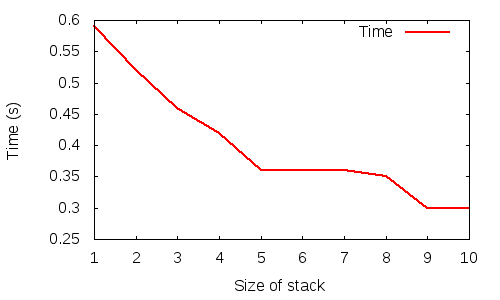
\includegraphics[width=\linewidth]{Shashkova/images/dfs_time.png}}
   \caption{Время работы программы в зависимости от величины стека c алгоритмом Mark (DFS)}
   \label{ris:dtime}   
   \center{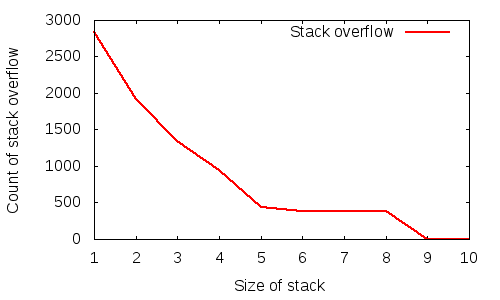
\includegraphics[width=\linewidth]{Shashkova/images/dfs_overflow_count.png}}
   \caption{Количество переполнений стека с алгоритмом Mark (DFS)}  
   \label{ris:dof}
   \end{figure}
   \begin{figure}
   \center{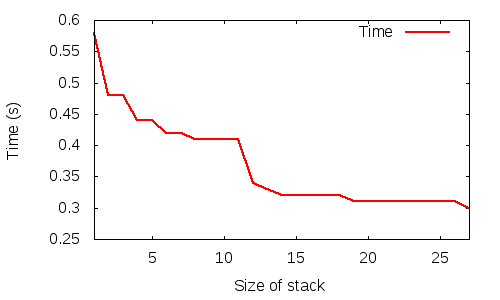
\includegraphics[width=\linewidth]{Shashkova/images/bfs_time.png}}
   \caption{Время работы программы в зависимости от величины стека c алгоритмом Mark (BFS)}
   \label{ris:btime}   
   \center{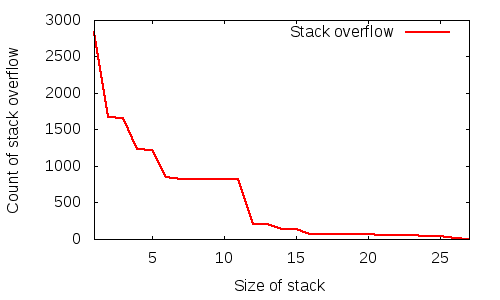
\includegraphics[width=\linewidth]{Shashkova/images/bfs_overflow_count.png}}
   \caption{Количество переполнений стека c алгоритмом Mark (BFS)}
   \label{ris:bof}
   \end{figure}
   

На рис.~\ref{ris:dof} показана зависимость количества переполнений стека от размера стека. Из этого графика хорошо видно, почему график времени работы имеет такую 
неравномерную структуру, а также «ступень». Становится понятно, что время работы программы с переполнениями стека напрямую зависит от количества этих переполнений,
которые происходили в процессе выполнения. И равномерное убывание времени на промежутке от 1 до 5, и постоянное время на промежутке от 5 до 8 полностью объясняется 
зависимостью количества переполнений, которая ведет себя аналогично.

Также были исследованы аналогичные зависимости для алгоритма маркировки с обходом объектов в ширину (Mark (BFS)).

На рис.~\ref{ris:btime} представлена зависимость времени работы программы от величины стека. 
При размере стека, большем 25, переполнения не происходит. Как и в случае с алгоритмом Mark (DFS) в худшем случае (при размере стека $n = 1$) время работы программы
увеличивается почти вдвое. Из особенностей графика можно отметить резкое падение времени работы при увеличении размера стека с 11 до 12. Аналогично для объяснения 
такой зависимости, рассмотрим поведение количества переполнений в зависимости от размера стека.

На рис.~\ref{ris:bof} показана зависимость количества переполнений стека от размера стека с алгоритмом Mark (BFS). Как и в случае с алгоритмом Mark (DFS), очевидно, 
что время работы напрямую зависит от количества происходящих переполнений стека. Резкое падение при изменении размера стека с 11 на 12 также объясняется количеством 
переполнений.

Объясним неравномерность количества переполнений, происходящих при работе каждого из алгоритмов. Будем называть {\it стековой глубиной } корневого объекта максимальную заполненность стека при обходе потомков данного 
корневого объекта.

На графиках рис.~\ref{ris:dm} и рис.~\ref{ris:bm} показано количество корневых объектов в зависимости от их стековой глубины для обоих алгоритмов. 
Из графика рис.~\ref{ris:dm} понятно поведение количества переполнений с алгоритмом Mark (DFS). Количество корневых 
объктов со стековой глубиной от 1 до 5 равномерно убывает, как и убывает количество переполнений. «Ступень» в количестве переполнений также связана с тем, 
что количество корневых объектов стековой глубины больше 5 очень мало по сравнению с объектами меньшей глубины. Поэтому количество переполнений почти не изменяется и 
убывает, только когда переполнения перестают возникать вовсе.

Аналогично для алгоритма Mark (BFS) из рис.~\ref{ris:bm} видно, что количество корневых объектов со стековой глубиной от 8 до 11 и больше 14 мало по сравнению с другими 
объектами, чем и объясняются постоянные промежутки на графике количества переполнений (рис.~\ref{ris:bof}).

   \begin{figure}[p!]   
   \center{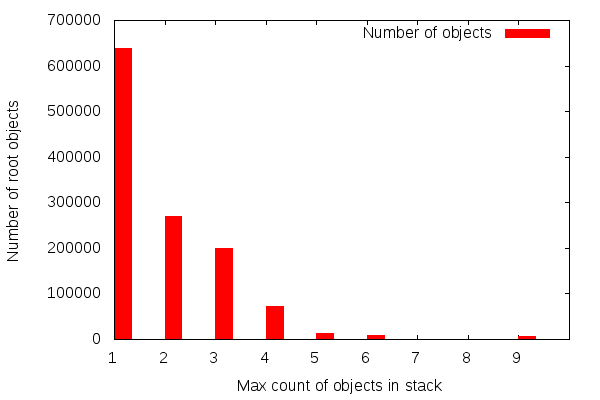
\includegraphics[width=\linewidth]{Shashkova/images/dfs_max_stack.png}}
   \caption{Количество корневых объектов в зависимости от глубины стека с алгоритмом Mark (DFS)}
   \label{ris:dm}   
   \center{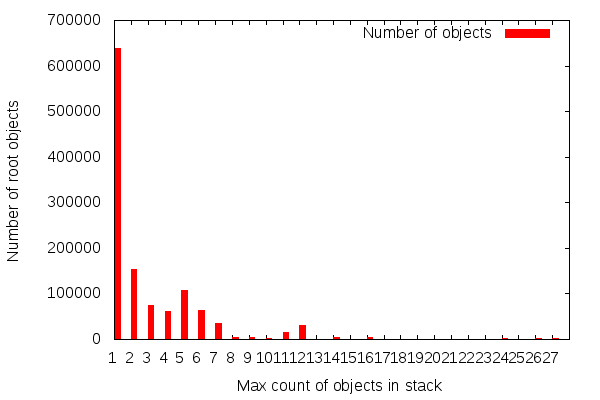
\includegraphics[width=\linewidth]{Shashkova/images/bfs_max_stack.png}}
   \caption{Количество корневых объектов в зависимости от глубины стека с алгоритмом Mark (BFS)}
   \label{ris:bm}   
   \end{figure}


Стоит обратить отдельное внимание на величину стека, при которой происходят переполнения в обоих алгоритмах. Как говорилось ранее, с использованием алгоритма
Mark (BFS) стек перестает переполнятся при размере, большем 9. С алгоритмом Mark (DFS) переполнения происходят вплоть до размера, равного 25. То есть при переходе 
к другому алгоритму размер стека увеличивается почти в 3 раза. Скорее всего, это связано со структурой объектов в тестовой программе. 

Граф, описывающий структуру наших объектов, является лесом из почти деревьев. Под почти деревьями будем понимать традиционные деревья, определенные в теории графов, 
с тем лишь 
отличием, что они могут содержать петли (вершины, связанные ребром сами с собой). Появление петель связано с наличием замыканий (closure) в множестве наших 
объектов. Однако наличие петель не влияет на глубину и ширину дерева, поэтому мы можем считать наши графы деревьями.

Такая значительная разница в размерах стека означает, что у многих деревьев их ширина больше глубины. Анализ объектов в тестовой программе показал, что 
количество потомков у объекта не превышает трех. Даже при небольшой глубине дерева количество объектов на каждом уровне растет довольно быстро, что и приводит 
к увеличению размера используемого стека при обходе в ширину, в отличие от обхода в глубину.

\section*{Заключение}

В результате работы была проведена интеграция бэкенда для языка OCaml и расширения для сборки мусора в LLVM. Было изучено внутреннее 
представление объектов в языке OCaml и реализованы два итеративных алгоритма обхода объектов в стадии пометки сборщика мусора. Результат работы был протестирован
на простейших программах и корректно работает на более сложных примерах. 

\begin{thebibliography}{99}
\bibitem{LLVM} Chris Lattner.
LLVM: An Infrastructure for Multi-Stage Optimization.
Computer Science Dept., University of Illinois at Urbana-Champaign, 2002.

\bibitem{samofal}
Самофалов А.В. Принципы организации сборщика мусора в инфраструктуре LLVM // 
Настоящий сборник.

\bibitem{knuth}
Д. Кнут. Искусство программирования, том 1. Основные алгоритмы.
М.: ``Вильямс»'', 2006.

\bibitem{pliss}
Плисс О.А. Материалы к летней школе ``Управление памятью''. СПбГУ, 2013.

\end{thebibliography}

\title{Сборщик мусора\\
для языка Objective Caml\\
в инфраструктуре LLVM}
%
\titlerunning{Сборщик мусора для языка Objective Caml}
\author{Шашкова Елизавета Михайловна}
%
\authorrunning{Е.М.Шашкова} % abbreviated author list (for running head)
%
%%%% list of authors for the TOC (use if author list has to be modified)
\tocauthor{Е.М.Шашкова}
%
\institute{Санкт-Петербургский государственный университет\\
\email{Elizabeth.Shashkova@gmail.com}}

\maketitle              % typeset the title of the contribution

\section*{Введение}

Сборка мусора --- одна из форм автоматического управления памятью. Специальный компонент поддержки среды времени исполнения, 
называемый сборщиком мусора, автоматически освобождает 
память, удаляя объекты, которые больше не являются доступными для использования.  Сборка мусора освобождает программиста от 
необходимости вручную выделять и освобождать память и позволяет сконцентрироваться на выполнении других задач.
В большинстве современных языков все чаще происходит отказ от предоставления явных средств управления памятью в пользу сборки мусора.

Сборка мусора тесно связана с реализацией компилятора: например, он должен предоставлять сборщику мусора способ определить адреса корневых объектов во
время исполнения. Один из основных
подходов к созданию компиляторов --- использование инфраструктур. Одной из таких инфраструктур построения компиляторов является LLVM 
(Low Level Virtual Machine)~\cite{LLVM}. 

LLVM предназначена 
для анализа, трансформации и оптимизации программ. В основе LLVM лежит промежуточное представление кода 
(Intermediate Representation, IR), над которым можно производить трансформации во время компиляции и компоновки. 
Из этого представления генерируется оптимизированный машинный код для целого ряда платформ.

Objective Caml (OCaml)\footnote{www.caml.inria.fr} --- современный объектно-ориентированный язык функционального программирования общего назначения.
Для языка OCaml существует единственный компилятор от разработчиков самого языка, однако он содержит довольно много платформозависимого кода.
LLVM улучшает переносимость кода между различными платформами и тем самым упрощает процесс построения 
собственного компилятора. Однако язык OCaml требует сборки мусора и реализованный для него бэкенд рассчитывает на наличие сборщика мусора. Но в 
инфраструктуре LLVM нет стандартного способа осуществления сборки мусора, и разработчики предоставили 
возможность для создания расширения LLVM, позволяющего её реализовывать. Данное расширение было реализовано в виде подключаемого модуля~\cite{samofal}.

Целью данной курсовой работы является проведение интеграции бэкенда для языка OCaml и расширения для сборки мусора в LLVM. Необходимо изучить внутреннее 
устройство объектов в языке OCaml и реализвать стадию пометки (mark) для алгоритма сборки мусора mark-and-sweep.

\section{Представление данных в OCaml}

Стадия пометки в алгоритме сборки мусора mark-and-sweep заключается в том, чтобы обойти все "живые" (всё ещё доступные из корневого множества)
объекты и пометить их. Затем на стадии очистки все объекты, которые не были помечены на данной стадии, будут считаться недоступными в программе, а значит,
будут подлежать удалению.

Для реализации стадии пометки необходимо узнать внутреннее устройство объектов.
Все значения в языке OCaml имеют единообразное представление: все они являются типом value языка C (это значение и макросы для работы с ним
определены в файле caml/mlvalues.h). Объект типа value может являться:

\begin{itemize}
   \item целым числом;
   \item указателем на блок внутри кучи;
   \item указателем на блоки вне кучи.
\end{itemize}

Целые числа находятся не в куче, поэтому сборщиком мусора рассматриваться не будут. Блоки, находящиеся в куче, являются основной целью работы сборщика
мусора. Каждый блок содержит заголовок с информацией о длине блока и теге.

Тег определяет структуру блока. Теги со значением меньше, чем \texttt{No\_scan\_tag}, 
означают, что данный блок является корректно структурированным и может быть рекурсивно обойден сборщиком мусора. 
Теги со значением больше, либо равные \texttt{No\_scan\_tag}, означают, что содержимое данного блока должно быть проигнорировано сборщиком мусора. 
Соответствие внутреннего содержимого блоков их тегам показано на рис.~\ref{block_types}.

\begin{figure}[t]
    \begin{tabular}{|l| p{6cm}|}
    \hline
    Тег & Содержимое блока \\
    \hline
    от 0 до \texttt{No\_scan\_tag} -- 1 & Структурированный блок (массив объектов OCaml). Каждое поле является типом value.\\
    \hline
    \texttt{Closure\_tag} & Замыкание представляет собой функциональное значение. Первое слово является указателем на участок кода,
    остальные являются объектами типа value.\\
    \hline
    \texttt{String\_tag} & Строка символов. \\
    \hline
    \texttt{Double\_tag} & Число с плавающей точкой двойной точности. \\
    \hline
    \texttt{Double\_array\_tag} & Массив чисел c плавающей точкой двойной точности. \\
    \hline
    \texttt{Abstract\_tag} & Блок, представляющий абстрактный тип данных. \\
    \hline
    \texttt{Custom\_tag} & Блок, представляющий абстрактный тип данных
    с ``привязанными'' пользовательскими функциями. \\
    \hline
    \end{tabular}
    \caption{Типы блоков в OCaml}
    \label{block_types}
\end{figure}

Благодаря такому устройству объектов становится возможным обход объектов, доступных из живых объектов. Можно быть уверенными,
что в процессе обхода мы не уйдем в область памяти, неинтересную сборщику мусора, а также не пропустим интересующие нас объекты. 

\section{Обход объектов}

Наиболее естественным алгоритмом обхода объектов можно назвать рекурсивный алгоритм. Его описание представлено ниже.
\begin{enumerate}
   \item Алгоритм запускается для каждого корневого объекта.
   \item Проверить, что текущий объект является блоком (а, например, не целым числом).
   \item Если объект является блоком, узнать значение его тега.
   \item Если значение тега меньше значения \texttt{No\_scan\_tag}, объект является живым. Нужно проверить, что
   данный объект находится в куче и пометить его как живой.
   \item Если значение тега больше или равно значению \texttt{No\_scan\_tag}, значит, объект должен игнорироваться сборщиком 
   мусора.
   \item После пометки самого объекта нужно последовательно обойти блоки, содержащиеся внутри данного блока 
   (их количество известно из заголовка) и повторить с ними ту же операцию.
   \item Отдельное внимание нужно уделить объекту с тегом \texttt{Closure\_tag}, так как первое слово является 
   указателем на код и при обходе сборщиком мусора должно игнорироваться.
\end{enumerate}

Однако, рекурсивный вызов функций потребует дополнительной памяти для сохранения стека вызовов, причем размер этого стека предсказать невозможно. Поэтому данный 
алгоритм необходимо было превратить в нерекурсивный, с использованием собственного стека. Структуру объектов программы можно представить в виде графа, где 
вершины --- объекты, а ребра --- ссылки между объектами. Граф можно обойти двумя способами: в ширину (Breadth-first search) и в глубину(Depth-first search).

При обходе в глубину у каждого объекта поочередно просматриваются объекты, на которые он ссылается. Для каждого такого объекта помечаются все его потомки и только 
потом алгоритм переходит к следующему потомку текущего объекта. Код Mark описывает данный алгоритм. Здесь $push()$ и $pop()$ --- операции работы со стеком.

\begin{algorithm}[p]
\caption{Mark}
\label{BFS}
\begin{algorithmic}[1]
    \For {$root \in root\_objects$}
        \If {$is\_object(root)$}
            \If {$tag(root) < No\_scan\_tag$ }
                \If {$root$ in heap}
                    \State {$mark(root)$}
                \EndIf
                \State $push(root)$
                \While {$object \leftarrow pop()$}
                    \State $size \leftarrow size(object)$
                    \If {$tag(object) = Closure\_tag$}
                        \State $i = 1$
                    \Else
                        \State $i = 0$
                    \EndIf
                    \For {$i < size$}
                        \State $child \leftarrow Field(object, i)$
                        \If {   $is\_object(child)$ and\\
                                \hskip\algorithmicindent
                                \hskip\algorithmicindent
                                \hskip\algorithmicindent
                                \hskip\algorithmicindent
                                \hskip\algorithmicindent
                                \hskip\algorithmicindent $tag(child) < No\_scan\_tag$                           
                             }
                            \If {$child$ in heap and not $marked(child)$}
                                \State {$mark(child)$}
                                \State {$push(child)$}
                            \EndIf
                        \EndIf
                    \EndFor
                \EndWhile
            \EndIf
        \EndIf
    \EndFor
    %\EndProcedure
\end{algorithmic}
\end{algorithm}


При обходе в ширину объекты рассматриваются в порядке возрастания расстояния от них до коневого объекта в графе объектов. Данный алгоритм описывается
так же, как и алгоритм Mark, с тем лишь отличием, что вместо стека используется очередь, реализованная на массиве. То есть в данном псевдокоде операции 
$push()$ и $pop()$ --- операции работы с очередью.

Обе модификации данного алгоритма (с обходом в глубину и в ширину) были реализованы итеративно с созданием стека в статической области памяти. 
Отсюда понятно, что размер стека в таком случае является постоянным, и может произойти переполнение стека. Для данной ситуации существует 
специальный алгоритм восстановления.

В случае переполнения стека нельзя допустить некорректную работу сборщика мусора. Если произойдет ошибка в работе стадии пометки, часть живых 
объектов не будут помечены, то есть будут считаться мертвыми и память из-под них будет преждевременно освобождена, что приведет к 
некорректной работе программы. Алгоритм восстановления при переполнении стека был описан в ~\cite{knuth}. Для реализации было решено использовать модификацию 
этого алгоритма~\cite{pliss}. Этот алгоритм, работающий с ограниченной памятью, можно описать следующим образом:

\begin{enumerate}
   \item При заполнении стека алгоритм пометки продолжает свою работу. Однако новые объекты, которые не поместились в стек, в него не добавляются,
   а просто игнорируются.
   \item При переполнении устанавливается специальный флаг, сообщающий о том, что переполнение произошло.
   \item При завершении стадии пометки проверяется состояние флага о переполнении.
   \item Если переполнение произошло, значит, часть живых объектов не была помечена. Начинается последовательный обход кучи.
   \item Флаг переполнения сбрасывается. Начиная с каждого помеченного (то есть точно живого) объекта кучи запускается алгоритм пометки.
   \item Теперь для пометки будет рассматриваться меньше объектов и велика вероятность, что они поместятся в стек. В случае же, если переполнение 
   произойдет снова, алгоритм повторится (снова установится флаг переполнения и т.д.).
\end{enumerate}

Нужно пояснить, что данный алгоритм не будет работать бесконечно долго, так как при каждом последующем запуске стадии пометки мы помечаем 
как минимум $n + 1$ объект из ранее не помеченных (где $n$ --- размер стека). Количество объектов в куче конечно, а значит, процесс когда-нибудь 
закончится. Все живые объекты будут помечены и стадия маркировки корректно выполнит свою задачу даже при условии переполнения стека.

\section{Результаты}
В результате был создан модуль, реализующий стадию маркировки для алгоритма сборки мусора и произведена модификация кучи для обработки переполнения стека.
Реализация была выполнена на языке C. 

Наиболее интересным было исследовать работу программы при переполнении стека. В качестве тестовой программы был взят парсер c С-подобного языка,
написанный на языке OCaml. Он принимает на вход файл для разбора и анализирует его. Во всех экспериментах, представленных ниже, на вход подавался
один и тот же файл. 

Сборка мусора вызывалась автоматически, использовался алгоритм инициализации, основанный на количестве доступной свободной памяти. Согласно 
этому алгоритму, сборка мусора начинается, когда объем занятой памяти в куче превышает некоторый порог, заданный переменной $Threshold$. В данных 
экспериментах значение переменной $Threshold$ равнялось 0.75, что соответствует моментам, когда 75\% объема памяти кучи заняты.  

Благодаря тому, что вызов сборки мусора основывался на количестве доступной памяти, во всех экспериментах количество вызовов сборки мусора было одинаково и равнялось 
1370. К тому же сборка мусора производилась на одинаковых стадиях работы программы.

На рис.~\ref{ris:dtime} представлена зависимость времени работы программы от
величины стека. При размере стека, большем 8, переполнения не происходит. Из графика видно, что переполнение стека значительно, почти в 2 раза, увеличивает 
время работы программы. Из графика видно, что время работы равномерно убывает при изменении размера стека от 1 до 5. При дальнейшем увеличении размера стека, 
на графике заметна некоторая «ступень»: при увеличении размера стека от 5 до 8 время работы программы почти не изменяется. И лишь после этого оно еще раз уменьшается 
и перестает зависеть от дальнейшего увеличения стека. 

Для исследования такого поведения, исследуем количество переполнений, происходящих при работе программы.

   \begin{figure}[p]   
   \center{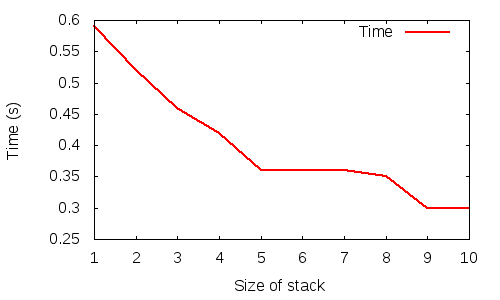
\includegraphics[width=\linewidth]{Shashkova/images/dfs_time.png}}
   \caption{Время работы программы в зависимости от величины стека c алгоритмом Mark (DFS)}
   \label{ris:dtime}   
   \center{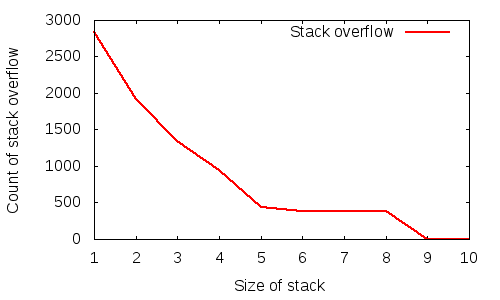
\includegraphics[width=\linewidth]{Shashkova/images/dfs_overflow_count.png}}
   \caption{Количество переполнений стека с алгоритмом Mark (DFS)}  
   \label{ris:dof}
   \end{figure}
   \begin{figure}
   \center{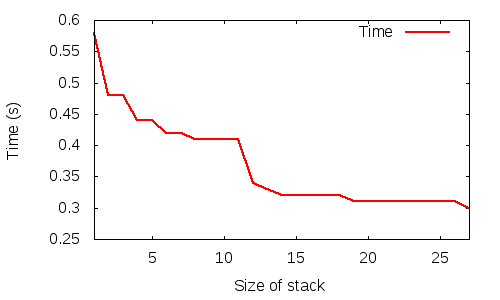
\includegraphics[width=\linewidth]{Shashkova/images/bfs_time.png}}
   \caption{Время работы программы в зависимости от величины стека c алгоритмом Mark (BFS)}
   \label{ris:btime}   
   \center{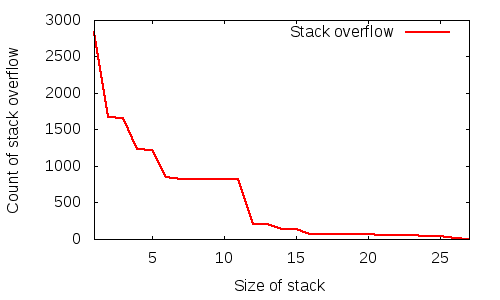
\includegraphics[width=\linewidth]{Shashkova/images/bfs_overflow_count.png}}
   \caption{Количество переполнений стека c алгоритмом Mark (BFS)}
   \label{ris:bof}
   \end{figure}
   

На рис.~\ref{ris:dof} показана зависимость количества переполнений стека от размера стека. Из этого графика хорошо видно, почему график времени работы имеет такую 
неравномерную структуру, а также «ступень». Становится понятно, что время работы программы с переполнениями стека напрямую зависит от количества этих переполнений,
которые происходили в процессе выполнения. И равномерное убывание времени на промежутке от 1 до 5, и постоянное время на промежутке от 5 до 8 полностью объясняется 
зависимостью количества переполнений, которая ведет себя аналогично.

Также были исследованы аналогичные зависимости для алгоритма маркировки с обходом объектов в ширину (Mark (BFS)).

На рис.~\ref{ris:btime} представлена зависимость времени работы программы от величины стека. 
При размере стека, большем 25, переполнения не происходит. Как и в случае с алгоритмом Mark (DFS) в худшем случае (при размере стека $n = 1$) время работы программы
увеличивается почти вдвое. Из особенностей графика можно отметить резкое падение времени работы при увеличении размера стека с 11 до 12. Аналогично для объяснения 
такой зависимости, рассмотрим поведение количества переполнений в зависимости от размера стека.

На рис.~\ref{ris:bof} показана зависимость количества переполнений стека от размера стека с алгоритмом Mark (BFS). Как и в случае с алгоритмом Mark (DFS), очевидно, 
что время работы напрямую зависит от количества происходящих переполнений стека. Резкое падение при изменении размера стека с 11 на 12 также объясняется количеством 
переполнений.

Объясним неравномерность количества переполнений, происходящих при работе каждого из алгоритмов. Будем называть {\it стековой глубиной } корневого объекта максимальную заполненность стека при обходе потомков данного 
корневого объекта.

На графиках рис.~\ref{ris:dm} и рис.~\ref{ris:bm} показано количество корневых объектов в зависимости от их стековой глубины для обоих алгоритмов. 
Из графика рис.~\ref{ris:dm} понятно поведение количества переполнений с алгоритмом Mark (DFS). Количество корневых 
объктов со стековой глубиной от 1 до 5 равномерно убывает, как и убывает количество переполнений. «Ступень» в количестве переполнений также связана с тем, 
что количество корневых объектов стековой глубины больше 5 очень мало по сравнению с объектами меньшей глубины. Поэтому количество переполнений почти не изменяется и 
убывает, только когда переполнения перестают возникать вовсе.

Аналогично для алгоритма Mark (BFS) из рис.~\ref{ris:bm} видно, что количество корневых объектов со стековой глубиной от 8 до 11 и больше 14 мало по сравнению с другими 
объектами, чем и объясняются постоянные промежутки на графике количества переполнений (рис.~\ref{ris:bof}).

   \begin{figure}[p!]   
   \center{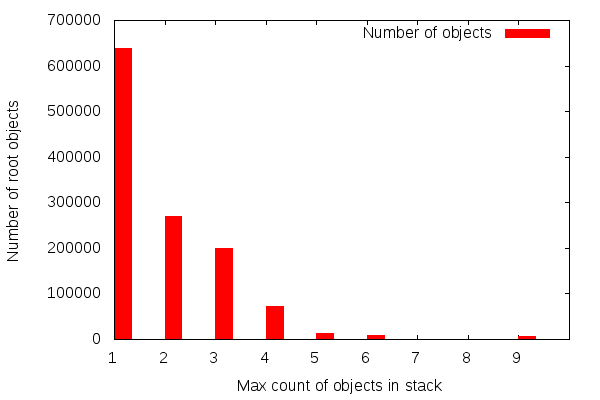
\includegraphics[width=\linewidth]{Shashkova/images/dfs_max_stack.png}}
   \caption{Количество корневых объектов в зависимости от глубины стека с алгоритмом Mark (DFS)}
   \label{ris:dm}   
   \center{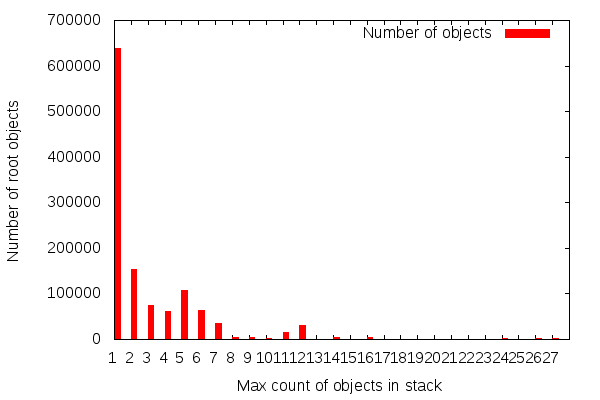
\includegraphics[width=\linewidth]{Shashkova/images/bfs_max_stack.png}}
   \caption{Количество корневых объектов в зависимости от глубины стека с алгоритмом Mark (BFS)}
   \label{ris:bm}   
   \end{figure}


Стоит обратить отдельное внимание на величину стека, при которой происходят переполнения в обоих алгоритмах. Как говорилось ранее, с использованием алгоритма
Mark (BFS) стек перестает переполнятся при размере, большем 9. С алгоритмом Mark (DFS) переполнения происходят вплоть до размера, равного 25. То есть при переходе 
к другому алгоритму размер стека увеличивается почти в 3 раза. Скорее всего, это связано со структурой объектов в тестовой программе. 

Граф, описывающий структуру наших объектов, является лесом из почти деревьев. Под почти деревьями будем понимать традиционные деревья, определенные в теории графов, 
с тем лишь 
отличием, что они могут содержать петли (вершины, связанные ребром сами с собой). Появление петель связано с наличием замыканий (closure) в множестве наших 
объектов. Однако наличие петель не влияет на глубину и ширину дерева, поэтому мы можем считать наши графы деревьями.

Такая значительная разница в размерах стека означает, что у многих деревьев их ширина больше глубины. Анализ объектов в тестовой программе показал, что 
количество потомков у объекта не превышает трех. Даже при небольшой глубине дерева количество объектов на каждом уровне растет довольно быстро, что и приводит 
к увеличению размера используемого стека при обходе в ширину, в отличие от обхода в глубину.

\section*{Заключение}

В результате работы была проведена интеграция бэкенда для языка OCaml и расширения для сборки мусора в LLVM. Было изучено внутреннее 
представление объектов в языке OCaml и реализованы два итеративных алгоритма обхода объектов в стадии пометки сборщика мусора. Результат работы был протестирован
на простейших программах и корректно работает на более сложных примерах. 

\begin{thebibliography}{99}
\bibitem{LLVM} Chris Lattner.
LLVM: An Infrastructure for Multi-Stage Optimization.
Computer Science Dept., University of Illinois at Urbana-Champaign, 2002.

\bibitem{samofal}
Самофалов А.В. Принципы организации сборщика мусора в инфраструктуре LLVM // 
Настоящий сборник.

\bibitem{knuth}
Д. Кнут. Искусство программирования, том 1. Основные алгоритмы.
М.: ``Вильямс»'', 2006.

\bibitem{pliss}
Плисс О.А. Материалы к летней школе ``Управление памятью''. СПбГУ, 2013.

\end{thebibliography}


\title{Сборщик мусора\\
для языка Objective Caml\\
в инфраструктуре LLVM}
%
\titlerunning{Сборщик мусора для языка Objective Caml}
\author{Шашкова Елизавета Михайловна}
%
\authorrunning{Е.М.Шашкова} % abbreviated author list (for running head)
%
%%%% list of authors for the TOC (use if author list has to be modified)
\tocauthor{Е.М.Шашкова}
%
\institute{Санкт-Петербургский государственный университет\\
\email{Elizabeth.Shashkova@gmail.com}}

\maketitle              % typeset the title of the contribution

\section*{Введение}

Сборка мусора --- одна из форм автоматического управления памятью. Специальный компонент поддержки среды времени исполнения, 
называемый сборщиком мусора, автоматически освобождает 
память, удаляя объекты, которые больше не являются доступными для использования.  Сборка мусора освобождает программиста от 
необходимости вручную выделять и освобождать память и позволяет сконцентрироваться на выполнении других задач.
В большинстве современных языков все чаще происходит отказ от предоставления явных средств управления памятью в пользу сборки мусора.

Сборка мусора тесно связана с реализацией компилятора: например, он должен предоставлять сборщику мусора способ определить адреса корневых объектов во
время исполнения. Один из основных
подходов к созданию компиляторов --- использование инфраструктур. Одной из таких инфраструктур построения компиляторов является LLVM 
(Low Level Virtual Machine)~\cite{LLVM}. 

LLVM предназначена 
для анализа, трансформации и оптимизации программ. В основе LLVM лежит промежуточное представление кода 
(Intermediate Representation, IR), над которым можно производить трансформации во время компиляции и компоновки. 
Из этого представления генерируется оптимизированный машинный код для целого ряда платформ.

Objective Caml (OCaml)\footnote{www.caml.inria.fr} --- современный объектно-ориентированный язык функционального программирования общего назначения.
Для языка OCaml существует единственный компилятор от разработчиков самого языка, однако он содержит довольно много платформозависимого кода.
LLVM улучшает переносимость кода между различными платформами и тем самым упрощает процесс построения 
собственного компилятора. Однако язык OCaml требует сборки мусора и реализованный для него бэкенд рассчитывает на наличие сборщика мусора. Но в 
инфраструктуре LLVM нет стандартного способа осуществления сборки мусора, и разработчики предоставили 
возможность для создания расширения LLVM, позволяющего её реализовывать. Данное расширение было реализовано в виде подключаемого модуля~\cite{samofal}.

Целью данной курсовой работы является проведение интеграции бэкенда для языка OCaml и расширения для сборки мусора в LLVM. Необходимо изучить внутреннее 
устройство объектов в языке OCaml и реализвать стадию пометки (mark) для алгоритма сборки мусора mark-and-sweep.

\section{Представление данных в OCaml}

Стадия пометки в алгоритме сборки мусора mark-and-sweep заключается в том, чтобы обойти все "живые" (всё ещё доступные из корневого множества)
объекты и пометить их. Затем на стадии очистки все объекты, которые не были помечены на данной стадии, будут считаться недоступными в программе, а значит,
будут подлежать удалению.

Для реализации стадии пометки необходимо узнать внутреннее устройство объектов.
Все значения в языке OCaml имеют единообразное представление: все они являются типом value языка C (это значение и макросы для работы с ним
определены в файле caml/mlvalues.h). Объект типа value может являться:

\begin{itemize}
   \item целым числом;
   \item указателем на блок внутри кучи;
   \item указателем на блоки вне кучи.
\end{itemize}

Целые числа находятся не в куче, поэтому сборщиком мусора рассматриваться не будут. Блоки, находящиеся в куче, являются основной целью работы сборщика
мусора. Каждый блок содержит заголовок с информацией о длине блока и теге.

Тег определяет структуру блока. Теги со значением меньше, чем \texttt{No\_scan\_tag}, 
означают, что данный блок является корректно структурированным и может быть рекурсивно обойден сборщиком мусора. 
Теги со значением больше, либо равные \texttt{No\_scan\_tag}, означают, что содержимое данного блока должно быть проигнорировано сборщиком мусора. 
Соответствие внутреннего содержимого блоков их тегам показано на рис.~\ref{block_types}.

\begin{figure}[t]
    \begin{tabular}{|l| p{6cm}|}
    \hline
    Тег & Содержимое блока \\
    \hline
    от 0 до \texttt{No\_scan\_tag} -- 1 & Структурированный блок (массив объектов OCaml). Каждое поле является типом value.\\
    \hline
    \texttt{Closure\_tag} & Замыкание представляет собой функциональное значение. Первое слово является указателем на участок кода,
    остальные являются объектами типа value.\\
    \hline
    \texttt{String\_tag} & Строка символов. \\
    \hline
    \texttt{Double\_tag} & Число с плавающей точкой двойной точности. \\
    \hline
    \texttt{Double\_array\_tag} & Массив чисел c плавающей точкой двойной точности. \\
    \hline
    \texttt{Abstract\_tag} & Блок, представляющий абстрактный тип данных. \\
    \hline
    \texttt{Custom\_tag} & Блок, представляющий абстрактный тип данных
    с ``привязанными'' пользовательскими функциями. \\
    \hline
    \end{tabular}
    \caption{Типы блоков в OCaml}
    \label{block_types}
\end{figure}

Благодаря такому устройству объектов становится возможным обход объектов, доступных из живых объектов. Можно быть уверенными,
что в процессе обхода мы не уйдем в область памяти, неинтересную сборщику мусора, а также не пропустим интересующие нас объекты. 

\section{Обход объектов}

Наиболее естественным алгоритмом обхода объектов можно назвать рекурсивный алгоритм. Его описание представлено ниже.
\begin{enumerate}
   \item Алгоритм запускается для каждого корневого объекта.
   \item Проверить, что текущий объект является блоком (а, например, не целым числом).
   \item Если объект является блоком, узнать значение его тега.
   \item Если значение тега меньше значения \texttt{No\_scan\_tag}, объект является живым. Нужно проверить, что
   данный объект находится в куче и пометить его как живой.
   \item Если значение тега больше или равно значению \texttt{No\_scan\_tag}, значит, объект должен игнорироваться сборщиком 
   мусора.
   \item После пометки самого объекта нужно последовательно обойти блоки, содержащиеся внутри данного блока 
   (их количество известно из заголовка) и повторить с ними ту же операцию.
   \item Отдельное внимание нужно уделить объекту с тегом \texttt{Closure\_tag}, так как первое слово является 
   указателем на код и при обходе сборщиком мусора должно игнорироваться.
\end{enumerate}

Однако, рекурсивный вызов функций потребует дополнительной памяти для сохранения стека вызовов, причем размер этого стека предсказать невозможно. Поэтому данный 
алгоритм необходимо было превратить в нерекурсивный, с использованием собственного стека. Структуру объектов программы можно представить в виде графа, где 
вершины --- объекты, а ребра --- ссылки между объектами. Граф можно обойти двумя способами: в ширину (Breadth-first search) и в глубину(Depth-first search).

При обходе в глубину у каждого объекта поочередно просматриваются объекты, на которые он ссылается. Для каждого такого объекта помечаются все его потомки и только 
потом алгоритм переходит к следующему потомку текущего объекта. Код Mark описывает данный алгоритм. Здесь $push()$ и $pop()$ --- операции работы со стеком.

\begin{algorithm}[p]
\caption{Mark}
\label{BFS}
\begin{algorithmic}[1]
    \For {$root \in root\_objects$}
        \If {$is\_object(root)$}
            \If {$tag(root) < No\_scan\_tag$ }
                \If {$root$ in heap}
                    \State {$mark(root)$}
                \EndIf
                \State $push(root)$
                \While {$object \leftarrow pop()$}
                    \State $size \leftarrow size(object)$
                    \If {$tag(object) = Closure\_tag$}
                        \State $i = 1$
                    \Else
                        \State $i = 0$
                    \EndIf
                    \For {$i < size$}
                        \State $child \leftarrow Field(object, i)$
                        \If {   $is\_object(child)$ and\\
                                \hskip\algorithmicindent
                                \hskip\algorithmicindent
                                \hskip\algorithmicindent
                                \hskip\algorithmicindent
                                \hskip\algorithmicindent
                                \hskip\algorithmicindent $tag(child) < No\_scan\_tag$                           
                             }
                            \If {$child$ in heap and not $marked(child)$}
                                \State {$mark(child)$}
                                \State {$push(child)$}
                            \EndIf
                        \EndIf
                    \EndFor
                \EndWhile
            \EndIf
        \EndIf
    \EndFor
    %\EndProcedure
\end{algorithmic}
\end{algorithm}


При обходе в ширину объекты рассматриваются в порядке возрастания расстояния от них до коневого объекта в графе объектов. Данный алгоритм описывается
так же, как и алгоритм Mark, с тем лишь отличием, что вместо стека используется очередь, реализованная на массиве. То есть в данном псевдокоде операции 
$push()$ и $pop()$ --- операции работы с очередью.

Обе модификации данного алгоритма (с обходом в глубину и в ширину) были реализованы итеративно с созданием стека в статической области памяти. 
Отсюда понятно, что размер стека в таком случае является постоянным, и может произойти переполнение стека. Для данной ситуации существует 
специальный алгоритм восстановления.

В случае переполнения стека нельзя допустить некорректную работу сборщика мусора. Если произойдет ошибка в работе стадии пометки, часть живых 
объектов не будут помечены, то есть будут считаться мертвыми и память из-под них будет преждевременно освобождена, что приведет к 
некорректной работе программы. Алгоритм восстановления при переполнении стека был описан в ~\cite{knuth}. Для реализации было решено использовать модификацию 
этого алгоритма~\cite{pliss}. Этот алгоритм, работающий с ограниченной памятью, можно описать следующим образом:

\begin{enumerate}
   \item При заполнении стека алгоритм пометки продолжает свою работу. Однако новые объекты, которые не поместились в стек, в него не добавляются,
   а просто игнорируются.
   \item При переполнении устанавливается специальный флаг, сообщающий о том, что переполнение произошло.
   \item При завершении стадии пометки проверяется состояние флага о переполнении.
   \item Если переполнение произошло, значит, часть живых объектов не была помечена. Начинается последовательный обход кучи.
   \item Флаг переполнения сбрасывается. Начиная с каждого помеченного (то есть точно живого) объекта кучи запускается алгоритм пометки.
   \item Теперь для пометки будет рассматриваться меньше объектов и велика вероятность, что они поместятся в стек. В случае же, если переполнение 
   произойдет снова, алгоритм повторится (снова установится флаг переполнения и т.д.).
\end{enumerate}

Нужно пояснить, что данный алгоритм не будет работать бесконечно долго, так как при каждом последующем запуске стадии пометки мы помечаем 
как минимум $n + 1$ объект из ранее не помеченных (где $n$ --- размер стека). Количество объектов в куче конечно, а значит, процесс когда-нибудь 
закончится. Все живые объекты будут помечены и стадия маркировки корректно выполнит свою задачу даже при условии переполнения стека.

\section{Результаты}
В результате был создан модуль, реализующий стадию маркировки для алгоритма сборки мусора и произведена модификация кучи для обработки переполнения стека.
Реализация была выполнена на языке C. 

Наиболее интересным было исследовать работу программы при переполнении стека. В качестве тестовой программы был взят парсер c С-подобного языка,
написанный на языке OCaml. Он принимает на вход файл для разбора и анализирует его. Во всех экспериментах, представленных ниже, на вход подавался
один и тот же файл. 

Сборка мусора вызывалась автоматически, использовался алгоритм инициализации, основанный на количестве доступной свободной памяти. Согласно 
этому алгоритму, сборка мусора начинается, когда объем занятой памяти в куче превышает некоторый порог, заданный переменной $Threshold$. В данных 
экспериментах значение переменной $Threshold$ равнялось 0.75, что соответствует моментам, когда 75\% объема памяти кучи заняты.  

Благодаря тому, что вызов сборки мусора основывался на количестве доступной памяти, во всех экспериментах количество вызовов сборки мусора было одинаково и равнялось 
1370. К тому же сборка мусора производилась на одинаковых стадиях работы программы.

На рис.~\ref{ris:dtime} представлена зависимость времени работы программы от
величины стека. При размере стека, большем 8, переполнения не происходит. Из графика видно, что переполнение стека значительно, почти в 2 раза, увеличивает 
время работы программы. Из графика видно, что время работы равномерно убывает при изменении размера стека от 1 до 5. При дальнейшем увеличении размера стека, 
на графике заметна некоторая «ступень»: при увеличении размера стека от 5 до 8 время работы программы почти не изменяется. И лишь после этого оно еще раз уменьшается 
и перестает зависеть от дальнейшего увеличения стека. 

Для исследования такого поведения, исследуем количество переполнений, происходящих при работе программы.

   \begin{figure}[p]   
   \center{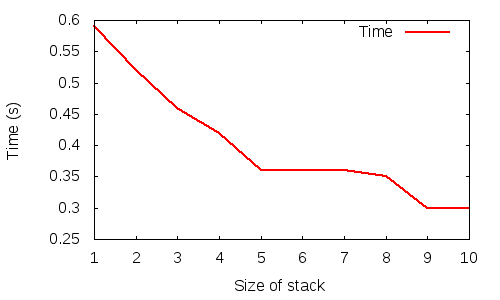
\includegraphics[width=\linewidth]{Shashkova/images/dfs_time.png}}
   \caption{Время работы программы в зависимости от величины стека c алгоритмом Mark (DFS)}
   \label{ris:dtime}   
   \center{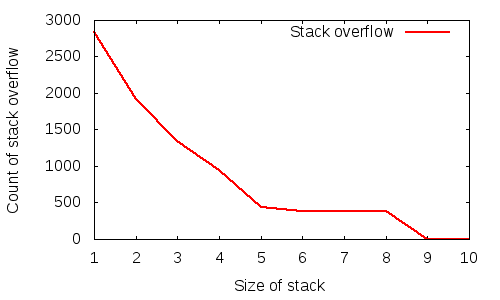
\includegraphics[width=\linewidth]{Shashkova/images/dfs_overflow_count.png}}
   \caption{Количество переполнений стека с алгоритмом Mark (DFS)}  
   \label{ris:dof}
   \end{figure}
   \begin{figure}
   \center{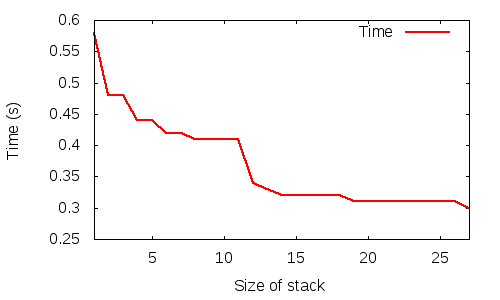
\includegraphics[width=\linewidth]{Shashkova/images/bfs_time.png}}
   \caption{Время работы программы в зависимости от величины стека c алгоритмом Mark (BFS)}
   \label{ris:btime}   
   \center{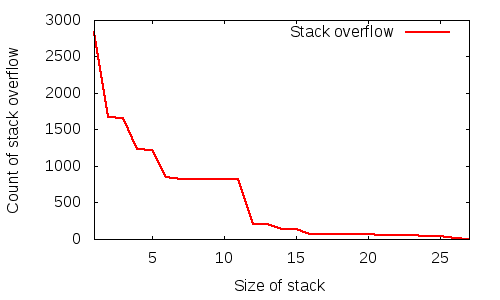
\includegraphics[width=\linewidth]{Shashkova/images/bfs_overflow_count.png}}
   \caption{Количество переполнений стека c алгоритмом Mark (BFS)}
   \label{ris:bof}
   \end{figure}
   

На рис.~\ref{ris:dof} показана зависимость количества переполнений стека от размера стека. Из этого графика хорошо видно, почему график времени работы имеет такую 
неравномерную структуру, а также «ступень». Становится понятно, что время работы программы с переполнениями стека напрямую зависит от количества этих переполнений,
которые происходили в процессе выполнения. И равномерное убывание времени на промежутке от 1 до 5, и постоянное время на промежутке от 5 до 8 полностью объясняется 
зависимостью количества переполнений, которая ведет себя аналогично.

Также были исследованы аналогичные зависимости для алгоритма маркировки с обходом объектов в ширину (Mark (BFS)).

На рис.~\ref{ris:btime} представлена зависимость времени работы программы от величины стека. 
При размере стека, большем 25, переполнения не происходит. Как и в случае с алгоритмом Mark (DFS) в худшем случае (при размере стека $n = 1$) время работы программы
увеличивается почти вдвое. Из особенностей графика можно отметить резкое падение времени работы при увеличении размера стека с 11 до 12. Аналогично для объяснения 
такой зависимости, рассмотрим поведение количества переполнений в зависимости от размера стека.

На рис.~\ref{ris:bof} показана зависимость количества переполнений стека от размера стека с алгоритмом Mark (BFS). Как и в случае с алгоритмом Mark (DFS), очевидно, 
что время работы напрямую зависит от количества происходящих переполнений стека. Резкое падение при изменении размера стека с 11 на 12 также объясняется количеством 
переполнений.

Объясним неравномерность количества переполнений, происходящих при работе каждого из алгоритмов. Будем называть {\it стековой глубиной } корневого объекта максимальную заполненность стека при обходе потомков данного 
корневого объекта.

На графиках рис.~\ref{ris:dm} и рис.~\ref{ris:bm} показано количество корневых объектов в зависимости от их стековой глубины для обоих алгоритмов. 
Из графика рис.~\ref{ris:dm} понятно поведение количества переполнений с алгоритмом Mark (DFS). Количество корневых 
объктов со стековой глубиной от 1 до 5 равномерно убывает, как и убывает количество переполнений. «Ступень» в количестве переполнений также связана с тем, 
что количество корневых объектов стековой глубины больше 5 очень мало по сравнению с объектами меньшей глубины. Поэтому количество переполнений почти не изменяется и 
убывает, только когда переполнения перестают возникать вовсе.

Аналогично для алгоритма Mark (BFS) из рис.~\ref{ris:bm} видно, что количество корневых объектов со стековой глубиной от 8 до 11 и больше 14 мало по сравнению с другими 
объектами, чем и объясняются постоянные промежутки на графике количества переполнений (рис.~\ref{ris:bof}).

   \begin{figure}[p!]   
   \center{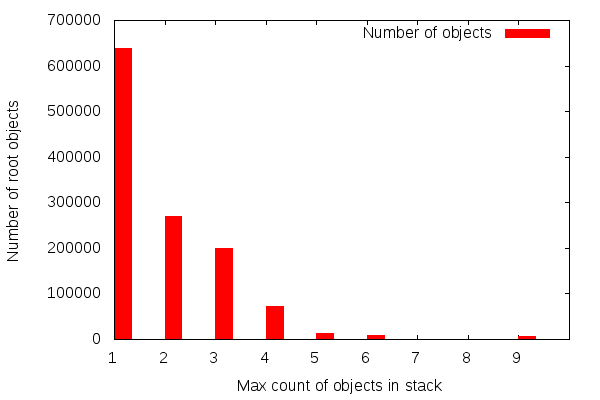
\includegraphics[width=\linewidth]{Shashkova/images/dfs_max_stack.png}}
   \caption{Количество корневых объектов в зависимости от глубины стека с алгоритмом Mark (DFS)}
   \label{ris:dm}   
   \center{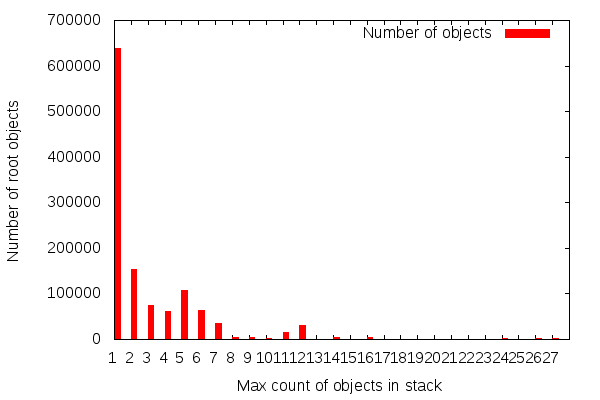
\includegraphics[width=\linewidth]{Shashkova/images/bfs_max_stack.png}}
   \caption{Количество корневых объектов в зависимости от глубины стека с алгоритмом Mark (BFS)}
   \label{ris:bm}   
   \end{figure}


Стоит обратить отдельное внимание на величину стека, при которой происходят переполнения в обоих алгоритмах. Как говорилось ранее, с использованием алгоритма
Mark (BFS) стек перестает переполнятся при размере, большем 9. С алгоритмом Mark (DFS) переполнения происходят вплоть до размера, равного 25. То есть при переходе 
к другому алгоритму размер стека увеличивается почти в 3 раза. Скорее всего, это связано со структурой объектов в тестовой программе. 

Граф, описывающий структуру наших объектов, является лесом из почти деревьев. Под почти деревьями будем понимать традиционные деревья, определенные в теории графов, 
с тем лишь 
отличием, что они могут содержать петли (вершины, связанные ребром сами с собой). Появление петель связано с наличием замыканий (closure) в множестве наших 
объектов. Однако наличие петель не влияет на глубину и ширину дерева, поэтому мы можем считать наши графы деревьями.

Такая значительная разница в размерах стека означает, что у многих деревьев их ширина больше глубины. Анализ объектов в тестовой программе показал, что 
количество потомков у объекта не превышает трех. Даже при небольшой глубине дерева количество объектов на каждом уровне растет довольно быстро, что и приводит 
к увеличению размера используемого стека при обходе в ширину, в отличие от обхода в глубину.

\section*{Заключение}

В результате работы была проведена интеграция бэкенда для языка OCaml и расширения для сборки мусора в LLVM. Было изучено внутреннее 
представление объектов в языке OCaml и реализованы два итеративных алгоритма обхода объектов в стадии пометки сборщика мусора. Результат работы был протестирован
на простейших программах и корректно работает на более сложных примерах. 

\begin{thebibliography}{99}
\bibitem{LLVM} Chris Lattner.
LLVM: An Infrastructure for Multi-Stage Optimization.
Computer Science Dept., University of Illinois at Urbana-Champaign, 2002.

\bibitem{samofal}
Самофалов А.В. Принципы организации сборщика мусора в инфраструктуре LLVM // 
Настоящий сборник.

\bibitem{knuth}
Д. Кнут. Искусство программирования, том 1. Основные алгоритмы.
М.: ``Вильямс»'', 2006.

\bibitem{pliss}
Плисс О.А. Материалы к летней школе ``Управление памятью''. СПбГУ, 2013.

\end{thebibliography}


\title{Сборщик мусора\\
для языка Objective Caml\\
в инфраструктуре LLVM}
%
\titlerunning{Сборщик мусора для языка Objective Caml}
\author{Шашкова Елизавета Михайловна}
%
\authorrunning{Е.М.Шашкова} % abbreviated author list (for running head)
%
%%%% list of authors for the TOC (use if author list has to be modified)
\tocauthor{Е.М.Шашкова}
%
\institute{Санкт-Петербургский государственный университет\\
\email{Elizabeth.Shashkova@gmail.com}}

\maketitle              % typeset the title of the contribution

\section*{Введение}

Сборка мусора --- одна из форм автоматического управления памятью. Специальный компонент поддержки среды времени исполнения, 
называемый сборщиком мусора, автоматически освобождает 
память, удаляя объекты, которые больше не являются доступными для использования.  Сборка мусора освобождает программиста от 
необходимости вручную выделять и освобождать память и позволяет сконцентрироваться на выполнении других задач.
В большинстве современных языков все чаще происходит отказ от предоставления явных средств управления памятью в пользу сборки мусора.

Сборка мусора тесно связана с реализацией компилятора: например, он должен предоставлять сборщику мусора способ определить адреса корневых объектов во
время исполнения. Один из основных
подходов к созданию компиляторов --- использование инфраструктур. Одной из таких инфраструктур построения компиляторов является LLVM 
(Low Level Virtual Machine)~\cite{LLVM}. 

LLVM предназначена 
для анализа, трансформации и оптимизации программ. В основе LLVM лежит промежуточное представление кода 
(Intermediate Representation, IR), над которым можно производить трансформации во время компиляции и компоновки. 
Из этого представления генерируется оптимизированный машинный код для целого ряда платформ.

Objective Caml (OCaml)\footnote{www.caml.inria.fr} --- современный объектно-ориентированный язык функционального программирования общего назначения.
Для языка OCaml существует единственный компилятор от разработчиков самого языка, однако он содержит довольно много платформозависимого кода.
LLVM улучшает переносимость кода между различными платформами и тем самым упрощает процесс построения 
собственного компилятора. Однако язык OCaml требует сборки мусора и реализованный для него бэкенд рассчитывает на наличие сборщика мусора. Но в 
инфраструктуре LLVM нет стандартного способа осуществления сборки мусора, и разработчики предоставили 
возможность для создания расширения LLVM, позволяющего её реализовывать. Данное расширение было реализовано в виде подключаемого модуля~\cite{samofal}.

Целью данной курсовой работы является проведение интеграции бэкенда для языка OCaml и расширения для сборки мусора в LLVM. Необходимо изучить внутреннее 
устройство объектов в языке OCaml и реализвать стадию пометки (mark) для алгоритма сборки мусора mark-and-sweep.

\section{Представление данных в OCaml}

Стадия пометки в алгоритме сборки мусора mark-and-sweep заключается в том, чтобы обойти все "живые" (всё ещё доступные из корневого множества)
объекты и пометить их. Затем на стадии очистки все объекты, которые не были помечены на данной стадии, будут считаться недоступными в программе, а значит,
будут подлежать удалению.

Для реализации стадии пометки необходимо узнать внутреннее устройство объектов.
Все значения в языке OCaml имеют единообразное представление: все они являются типом value языка C (это значение и макросы для работы с ним
определены в файле caml/mlvalues.h). Объект типа value может являться:

\begin{itemize}
   \item целым числом;
   \item указателем на блок внутри кучи;
   \item указателем на блоки вне кучи.
\end{itemize}

Целые числа находятся не в куче, поэтому сборщиком мусора рассматриваться не будут. Блоки, находящиеся в куче, являются основной целью работы сборщика
мусора. Каждый блок содержит заголовок с информацией о длине блока и теге.

Тег определяет структуру блока. Теги со значением меньше, чем \texttt{No\_scan\_tag}, 
означают, что данный блок является корректно структурированным и может быть рекурсивно обойден сборщиком мусора. 
Теги со значением больше, либо равные \texttt{No\_scan\_tag}, означают, что содержимое данного блока должно быть проигнорировано сборщиком мусора. 
Соответствие внутреннего содержимого блоков их тегам показано на рис.~\ref{block_types}.

\begin{figure}[t]
    \begin{tabular}{|l| p{6cm}|}
    \hline
    Тег & Содержимое блока \\
    \hline
    от 0 до \texttt{No\_scan\_tag} -- 1 & Структурированный блок (массив объектов OCaml). Каждое поле является типом value.\\
    \hline
    \texttt{Closure\_tag} & Замыкание представляет собой функциональное значение. Первое слово является указателем на участок кода,
    остальные являются объектами типа value.\\
    \hline
    \texttt{String\_tag} & Строка символов. \\
    \hline
    \texttt{Double\_tag} & Число с плавающей точкой двойной точности. \\
    \hline
    \texttt{Double\_array\_tag} & Массив чисел c плавающей точкой двойной точности. \\
    \hline
    \texttt{Abstract\_tag} & Блок, представляющий абстрактный тип данных. \\
    \hline
    \texttt{Custom\_tag} & Блок, представляющий абстрактный тип данных
    с ``привязанными'' пользовательскими функциями. \\
    \hline
    \end{tabular}
    \caption{Типы блоков в OCaml}
    \label{block_types}
\end{figure}

Благодаря такому устройству объектов становится возможным обход объектов, доступных из живых объектов. Можно быть уверенными,
что в процессе обхода мы не уйдем в область памяти, неинтересную сборщику мусора, а также не пропустим интересующие нас объекты. 

\section{Обход объектов}

Наиболее естественным алгоритмом обхода объектов можно назвать рекурсивный алгоритм. Его описание представлено ниже.
\begin{enumerate}
   \item Алгоритм запускается для каждого корневого объекта.
   \item Проверить, что текущий объект является блоком (а, например, не целым числом).
   \item Если объект является блоком, узнать значение его тега.
   \item Если значение тега меньше значения \texttt{No\_scan\_tag}, объект является живым. Нужно проверить, что
   данный объект находится в куче и пометить его как живой.
   \item Если значение тега больше или равно значению \texttt{No\_scan\_tag}, значит, объект должен игнорироваться сборщиком 
   мусора.
   \item После пометки самого объекта нужно последовательно обойти блоки, содержащиеся внутри данного блока 
   (их количество известно из заголовка) и повторить с ними ту же операцию.
   \item Отдельное внимание нужно уделить объекту с тегом \texttt{Closure\_tag}, так как первое слово является 
   указателем на код и при обходе сборщиком мусора должно игнорироваться.
\end{enumerate}

Однако, рекурсивный вызов функций потребует дополнительной памяти для сохранения стека вызовов, причем размер этого стека предсказать невозможно. Поэтому данный 
алгоритм необходимо было превратить в нерекурсивный, с использованием собственного стека. Структуру объектов программы можно представить в виде графа, где 
вершины --- объекты, а ребра --- ссылки между объектами. Граф можно обойти двумя способами: в ширину (Breadth-first search) и в глубину(Depth-first search).

При обходе в глубину у каждого объекта поочередно просматриваются объекты, на которые он ссылается. Для каждого такого объекта помечаются все его потомки и только 
потом алгоритм переходит к следующему потомку текущего объекта. Код Mark описывает данный алгоритм. Здесь $push()$ и $pop()$ --- операции работы со стеком.

\begin{algorithm}[p]
\caption{Mark}
\label{BFS}
\begin{algorithmic}[1]
    \For {$root \in root\_objects$}
        \If {$is\_object(root)$}
            \If {$tag(root) < No\_scan\_tag$ }
                \If {$root$ in heap}
                    \State {$mark(root)$}
                \EndIf
                \State $push(root)$
                \While {$object \leftarrow pop()$}
                    \State $size \leftarrow size(object)$
                    \If {$tag(object) = Closure\_tag$}
                        \State $i = 1$
                    \Else
                        \State $i = 0$
                    \EndIf
                    \For {$i < size$}
                        \State $child \leftarrow Field(object, i)$
                        \If {   $is\_object(child)$ and\\
                                \hskip\algorithmicindent
                                \hskip\algorithmicindent
                                \hskip\algorithmicindent
                                \hskip\algorithmicindent
                                \hskip\algorithmicindent
                                \hskip\algorithmicindent $tag(child) < No\_scan\_tag$                           
                             }
                            \If {$child$ in heap and not $marked(child)$}
                                \State {$mark(child)$}
                                \State {$push(child)$}
                            \EndIf
                        \EndIf
                    \EndFor
                \EndWhile
            \EndIf
        \EndIf
    \EndFor
    %\EndProcedure
\end{algorithmic}
\end{algorithm}


При обходе в ширину объекты рассматриваются в порядке возрастания расстояния от них до коневого объекта в графе объектов. Данный алгоритм описывается
так же, как и алгоритм Mark, с тем лишь отличием, что вместо стека используется очередь, реализованная на массиве. То есть в данном псевдокоде операции 
$push()$ и $pop()$ --- операции работы с очередью.

Обе модификации данного алгоритма (с обходом в глубину и в ширину) были реализованы итеративно с созданием стека в статической области памяти. 
Отсюда понятно, что размер стека в таком случае является постоянным, и может произойти переполнение стека. Для данной ситуации существует 
специальный алгоритм восстановления.

В случае переполнения стека нельзя допустить некорректную работу сборщика мусора. Если произойдет ошибка в работе стадии пометки, часть живых 
объектов не будут помечены, то есть будут считаться мертвыми и память из-под них будет преждевременно освобождена, что приведет к 
некорректной работе программы. Алгоритм восстановления при переполнении стека был описан в ~\cite{knuth}. Для реализации было решено использовать модификацию 
этого алгоритма~\cite{pliss}. Этот алгоритм, работающий с ограниченной памятью, можно описать следующим образом:

\begin{enumerate}
   \item При заполнении стека алгоритм пометки продолжает свою работу. Однако новые объекты, которые не поместились в стек, в него не добавляются,
   а просто игнорируются.
   \item При переполнении устанавливается специальный флаг, сообщающий о том, что переполнение произошло.
   \item При завершении стадии пометки проверяется состояние флага о переполнении.
   \item Если переполнение произошло, значит, часть живых объектов не была помечена. Начинается последовательный обход кучи.
   \item Флаг переполнения сбрасывается. Начиная с каждого помеченного (то есть точно живого) объекта кучи запускается алгоритм пометки.
   \item Теперь для пометки будет рассматриваться меньше объектов и велика вероятность, что они поместятся в стек. В случае же, если переполнение 
   произойдет снова, алгоритм повторится (снова установится флаг переполнения и т.д.).
\end{enumerate}

Нужно пояснить, что данный алгоритм не будет работать бесконечно долго, так как при каждом последующем запуске стадии пометки мы помечаем 
как минимум $n + 1$ объект из ранее не помеченных (где $n$ --- размер стека). Количество объектов в куче конечно, а значит, процесс когда-нибудь 
закончится. Все живые объекты будут помечены и стадия маркировки корректно выполнит свою задачу даже при условии переполнения стека.

\section{Результаты}
В результате был создан модуль, реализующий стадию маркировки для алгоритма сборки мусора и произведена модификация кучи для обработки переполнения стека.
Реализация была выполнена на языке C. 

Наиболее интересным было исследовать работу программы при переполнении стека. В качестве тестовой программы был взят парсер c С-подобного языка,
написанный на языке OCaml. Он принимает на вход файл для разбора и анализирует его. Во всех экспериментах, представленных ниже, на вход подавался
один и тот же файл. 

Сборка мусора вызывалась автоматически, использовался алгоритм инициализации, основанный на количестве доступной свободной памяти. Согласно 
этому алгоритму, сборка мусора начинается, когда объем занятой памяти в куче превышает некоторый порог, заданный переменной $Threshold$. В данных 
экспериментах значение переменной $Threshold$ равнялось 0.75, что соответствует моментам, когда 75\% объема памяти кучи заняты.  

Благодаря тому, что вызов сборки мусора основывался на количестве доступной памяти, во всех экспериментах количество вызовов сборки мусора было одинаково и равнялось 
1370. К тому же сборка мусора производилась на одинаковых стадиях работы программы.

На рис.~\ref{ris:dtime} представлена зависимость времени работы программы от
величины стека. При размере стека, большем 8, переполнения не происходит. Из графика видно, что переполнение стека значительно, почти в 2 раза, увеличивает 
время работы программы. Из графика видно, что время работы равномерно убывает при изменении размера стека от 1 до 5. При дальнейшем увеличении размера стека, 
на графике заметна некоторая «ступень»: при увеличении размера стека от 5 до 8 время работы программы почти не изменяется. И лишь после этого оно еще раз уменьшается 
и перестает зависеть от дальнейшего увеличения стека. 

Для исследования такого поведения, исследуем количество переполнений, происходящих при работе программы.

   \begin{figure}[p]   
   \center{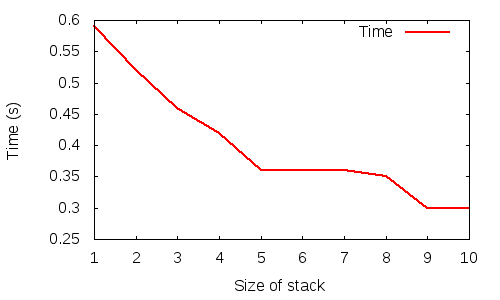
\includegraphics[width=\linewidth]{Shashkova/images/dfs_time.png}}
   \caption{Время работы программы в зависимости от величины стека c алгоритмом Mark (DFS)}
   \label{ris:dtime}   
   \center{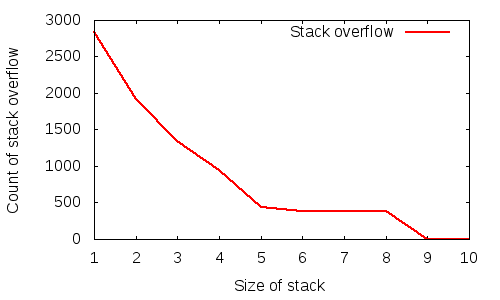
\includegraphics[width=\linewidth]{Shashkova/images/dfs_overflow_count.png}}
   \caption{Количество переполнений стека с алгоритмом Mark (DFS)}  
   \label{ris:dof}
   \end{figure}
   \begin{figure}
   \center{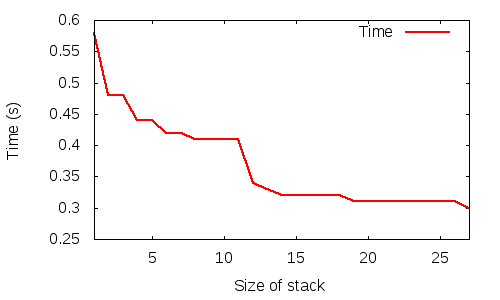
\includegraphics[width=\linewidth]{Shashkova/images/bfs_time.png}}
   \caption{Время работы программы в зависимости от величины стека c алгоритмом Mark (BFS)}
   \label{ris:btime}   
   \center{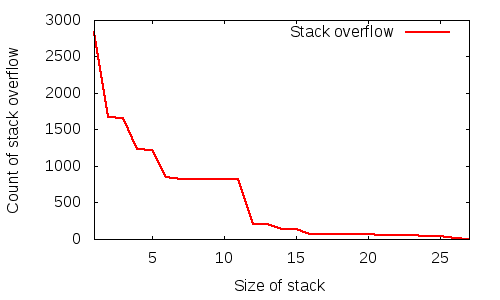
\includegraphics[width=\linewidth]{Shashkova/images/bfs_overflow_count.png}}
   \caption{Количество переполнений стека c алгоритмом Mark (BFS)}
   \label{ris:bof}
   \end{figure}
   

На рис.~\ref{ris:dof} показана зависимость количества переполнений стека от размера стека. Из этого графика хорошо видно, почему график времени работы имеет такую 
неравномерную структуру, а также «ступень». Становится понятно, что время работы программы с переполнениями стека напрямую зависит от количества этих переполнений,
которые происходили в процессе выполнения. И равномерное убывание времени на промежутке от 1 до 5, и постоянное время на промежутке от 5 до 8 полностью объясняется 
зависимостью количества переполнений, которая ведет себя аналогично.

Также были исследованы аналогичные зависимости для алгоритма маркировки с обходом объектов в ширину (Mark (BFS)).

На рис.~\ref{ris:btime} представлена зависимость времени работы программы от величины стека. 
При размере стека, большем 25, переполнения не происходит. Как и в случае с алгоритмом Mark (DFS) в худшем случае (при размере стека $n = 1$) время работы программы
увеличивается почти вдвое. Из особенностей графика можно отметить резкое падение времени работы при увеличении размера стека с 11 до 12. Аналогично для объяснения 
такой зависимости, рассмотрим поведение количества переполнений в зависимости от размера стека.

На рис.~\ref{ris:bof} показана зависимость количества переполнений стека от размера стека с алгоритмом Mark (BFS). Как и в случае с алгоритмом Mark (DFS), очевидно, 
что время работы напрямую зависит от количества происходящих переполнений стека. Резкое падение при изменении размера стека с 11 на 12 также объясняется количеством 
переполнений.

Объясним неравномерность количества переполнений, происходящих при работе каждого из алгоритмов. Будем называть {\it стековой глубиной } корневого объекта максимальную заполненность стека при обходе потомков данного 
корневого объекта.

На графиках рис.~\ref{ris:dm} и рис.~\ref{ris:bm} показано количество корневых объектов в зависимости от их стековой глубины для обоих алгоритмов. 
Из графика рис.~\ref{ris:dm} понятно поведение количества переполнений с алгоритмом Mark (DFS). Количество корневых 
объктов со стековой глубиной от 1 до 5 равномерно убывает, как и убывает количество переполнений. «Ступень» в количестве переполнений также связана с тем, 
что количество корневых объектов стековой глубины больше 5 очень мало по сравнению с объектами меньшей глубины. Поэтому количество переполнений почти не изменяется и 
убывает, только когда переполнения перестают возникать вовсе.

Аналогично для алгоритма Mark (BFS) из рис.~\ref{ris:bm} видно, что количество корневых объектов со стековой глубиной от 8 до 11 и больше 14 мало по сравнению с другими 
объектами, чем и объясняются постоянные промежутки на графике количества переполнений (рис.~\ref{ris:bof}).

   \begin{figure}[p!]   
   \center{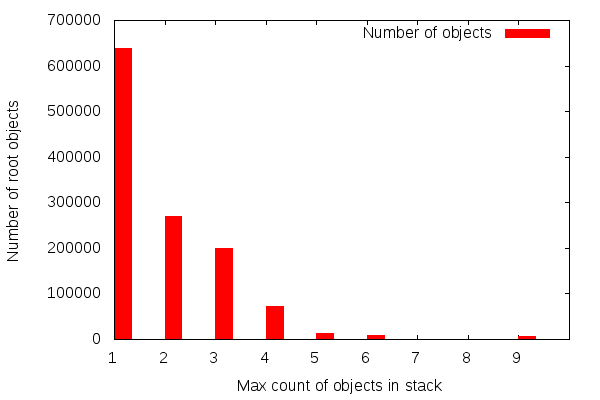
\includegraphics[width=\linewidth]{Shashkova/images/dfs_max_stack.png}}
   \caption{Количество корневых объектов в зависимости от глубины стека с алгоритмом Mark (DFS)}
   \label{ris:dm}   
   \center{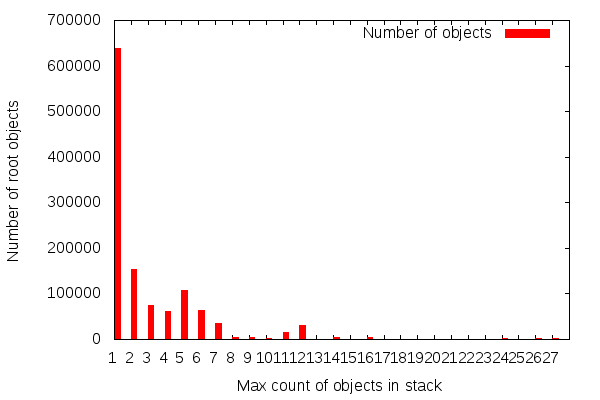
\includegraphics[width=\linewidth]{Shashkova/images/bfs_max_stack.png}}
   \caption{Количество корневых объектов в зависимости от глубины стека с алгоритмом Mark (BFS)}
   \label{ris:bm}   
   \end{figure}


Стоит обратить отдельное внимание на величину стека, при которой происходят переполнения в обоих алгоритмах. Как говорилось ранее, с использованием алгоритма
Mark (BFS) стек перестает переполнятся при размере, большем 9. С алгоритмом Mark (DFS) переполнения происходят вплоть до размера, равного 25. То есть при переходе 
к другому алгоритму размер стека увеличивается почти в 3 раза. Скорее всего, это связано со структурой объектов в тестовой программе. 

Граф, описывающий структуру наших объектов, является лесом из почти деревьев. Под почти деревьями будем понимать традиционные деревья, определенные в теории графов, 
с тем лишь 
отличием, что они могут содержать петли (вершины, связанные ребром сами с собой). Появление петель связано с наличием замыканий (closure) в множестве наших 
объектов. Однако наличие петель не влияет на глубину и ширину дерева, поэтому мы можем считать наши графы деревьями.

Такая значительная разница в размерах стека означает, что у многих деревьев их ширина больше глубины. Анализ объектов в тестовой программе показал, что 
количество потомков у объекта не превышает трех. Даже при небольшой глубине дерева количество объектов на каждом уровне растет довольно быстро, что и приводит 
к увеличению размера используемого стека при обходе в ширину, в отличие от обхода в глубину.

\section*{Заключение}

В результате работы была проведена интеграция бэкенда для языка OCaml и расширения для сборки мусора в LLVM. Было изучено внутреннее 
представление объектов в языке OCaml и реализованы два итеративных алгоритма обхода объектов в стадии пометки сборщика мусора. Результат работы был протестирован
на простейших программах и корректно работает на более сложных примерах. 

\begin{thebibliography}{99}
\bibitem{LLVM} Chris Lattner.
LLVM: An Infrastructure for Multi-Stage Optimization.
Computer Science Dept., University of Illinois at Urbana-Champaign, 2002.

\bibitem{samofal}
Самофалов А.В. Принципы организации сборщика мусора в инфраструктуре LLVM // 
Настоящий сборник.

\bibitem{knuth}
Д. Кнут. Искусство программирования, том 1. Основные алгоритмы.
М.: ``Вильямс»'', 2006.

\bibitem{pliss}
Плисс О.А. Материалы к летней школе ``Управление памятью''. СПбГУ, 2013.

\end{thebibliography}


\title{Сборщик мусора\\
для языка Objective Caml\\
в инфраструктуре LLVM}
%
\titlerunning{Сборщик мусора для языка Objective Caml}
\author{Шашкова Елизавета Михайловна}
%
\authorrunning{Е.М.Шашкова} % abbreviated author list (for running head)
%
%%%% list of authors for the TOC (use if author list has to be modified)
\tocauthor{Е.М.Шашкова}
%
\institute{Санкт-Петербургский государственный университет\\
\email{Elizabeth.Shashkova@gmail.com}}

\maketitle              % typeset the title of the contribution

\section*{Введение}

Сборка мусора --- одна из форм автоматического управления памятью. Специальный компонент поддержки среды времени исполнения, 
называемый сборщиком мусора, автоматически освобождает 
память, удаляя объекты, которые больше не являются доступными для использования.  Сборка мусора освобождает программиста от 
необходимости вручную выделять и освобождать память и позволяет сконцентрироваться на выполнении других задач.
В большинстве современных языков все чаще происходит отказ от предоставления явных средств управления памятью в пользу сборки мусора.

Сборка мусора тесно связана с реализацией компилятора: например, он должен предоставлять сборщику мусора способ определить адреса корневых объектов во
время исполнения. Один из основных
подходов к созданию компиляторов --- использование инфраструктур. Одной из таких инфраструктур построения компиляторов является LLVM 
(Low Level Virtual Machine)~\cite{LLVM}. 

LLVM предназначена 
для анализа, трансформации и оптимизации программ. В основе LLVM лежит промежуточное представление кода 
(Intermediate Representation, IR), над которым можно производить трансформации во время компиляции и компоновки. 
Из этого представления генерируется оптимизированный машинный код для целого ряда платформ.

Objective Caml (OCaml)\footnote{www.caml.inria.fr} --- современный объектно-ориентированный язык функционального программирования общего назначения.
Для языка OCaml существует единственный компилятор от разработчиков самого языка, однако он содержит довольно много платформозависимого кода.
LLVM улучшает переносимость кода между различными платформами и тем самым упрощает процесс построения 
собственного компилятора. Однако язык OCaml требует сборки мусора и реализованный для него бэкенд рассчитывает на наличие сборщика мусора. Но в 
инфраструктуре LLVM нет стандартного способа осуществления сборки мусора, и разработчики предоставили 
возможность для создания расширения LLVM, позволяющего её реализовывать. Данное расширение было реализовано в виде подключаемого модуля~\cite{samofal}.

Целью данной курсовой работы является проведение интеграции бэкенда для языка OCaml и расширения для сборки мусора в LLVM. Необходимо изучить внутреннее 
устройство объектов в языке OCaml и реализвать стадию пометки (mark) для алгоритма сборки мусора mark-and-sweep.

\section{Представление данных в OCaml}

Стадия пометки в алгоритме сборки мусора mark-and-sweep заключается в том, чтобы обойти все "живые" (всё ещё доступные из корневого множества)
объекты и пометить их. Затем на стадии очистки все объекты, которые не были помечены на данной стадии, будут считаться недоступными в программе, а значит,
будут подлежать удалению.

Для реализации стадии пометки необходимо узнать внутреннее устройство объектов.
Все значения в языке OCaml имеют единообразное представление: все они являются типом value языка C (это значение и макросы для работы с ним
определены в файле caml/mlvalues.h). Объект типа value может являться:

\begin{itemize}
   \item целым числом;
   \item указателем на блок внутри кучи;
   \item указателем на блоки вне кучи.
\end{itemize}

Целые числа находятся не в куче, поэтому сборщиком мусора рассматриваться не будут. Блоки, находящиеся в куче, являются основной целью работы сборщика
мусора. Каждый блок содержит заголовок с информацией о длине блока и теге.

Тег определяет структуру блока. Теги со значением меньше, чем \texttt{No\_scan\_tag}, 
означают, что данный блок является корректно структурированным и может быть рекурсивно обойден сборщиком мусора. 
Теги со значением больше, либо равные \texttt{No\_scan\_tag}, означают, что содержимое данного блока должно быть проигнорировано сборщиком мусора. 
Соответствие внутреннего содержимого блоков их тегам показано на рис.~\ref{block_types}.

\begin{figure}[t]
    \begin{tabular}{|l| p{6cm}|}
    \hline
    Тег & Содержимое блока \\
    \hline
    от 0 до \texttt{No\_scan\_tag} -- 1 & Структурированный блок (массив объектов OCaml). Каждое поле является типом value.\\
    \hline
    \texttt{Closure\_tag} & Замыкание представляет собой функциональное значение. Первое слово является указателем на участок кода,
    остальные являются объектами типа value.\\
    \hline
    \texttt{String\_tag} & Строка символов. \\
    \hline
    \texttt{Double\_tag} & Число с плавающей точкой двойной точности. \\
    \hline
    \texttt{Double\_array\_tag} & Массив чисел c плавающей точкой двойной точности. \\
    \hline
    \texttt{Abstract\_tag} & Блок, представляющий абстрактный тип данных. \\
    \hline
    \texttt{Custom\_tag} & Блок, представляющий абстрактный тип данных
    с ``привязанными'' пользовательскими функциями. \\
    \hline
    \end{tabular}
    \caption{Типы блоков в OCaml}
    \label{block_types}
\end{figure}

Благодаря такому устройству объектов становится возможным обход объектов, доступных из живых объектов. Можно быть уверенными,
что в процессе обхода мы не уйдем в область памяти, неинтересную сборщику мусора, а также не пропустим интересующие нас объекты. 

\section{Обход объектов}

Наиболее естественным алгоритмом обхода объектов можно назвать рекурсивный алгоритм. Его описание представлено ниже.
\begin{enumerate}
   \item Алгоритм запускается для каждого корневого объекта.
   \item Проверить, что текущий объект является блоком (а, например, не целым числом).
   \item Если объект является блоком, узнать значение его тега.
   \item Если значение тега меньше значения \texttt{No\_scan\_tag}, объект является живым. Нужно проверить, что
   данный объект находится в куче и пометить его как живой.
   \item Если значение тега больше или равно значению \texttt{No\_scan\_tag}, значит, объект должен игнорироваться сборщиком 
   мусора.
   \item После пометки самого объекта нужно последовательно обойти блоки, содержащиеся внутри данного блока 
   (их количество известно из заголовка) и повторить с ними ту же операцию.
   \item Отдельное внимание нужно уделить объекту с тегом \texttt{Closure\_tag}, так как первое слово является 
   указателем на код и при обходе сборщиком мусора должно игнорироваться.
\end{enumerate}

Однако, рекурсивный вызов функций потребует дополнительной памяти для сохранения стека вызовов, причем размер этого стека предсказать невозможно. Поэтому данный 
алгоритм необходимо было превратить в нерекурсивный, с использованием собственного стека. Структуру объектов программы можно представить в виде графа, где 
вершины --- объекты, а ребра --- ссылки между объектами. Граф можно обойти двумя способами: в ширину (Breadth-first search) и в глубину(Depth-first search).

При обходе в глубину у каждого объекта поочередно просматриваются объекты, на которые он ссылается. Для каждого такого объекта помечаются все его потомки и только 
потом алгоритм переходит к следующему потомку текущего объекта. Код Mark описывает данный алгоритм. Здесь $push()$ и $pop()$ --- операции работы со стеком.

\begin{algorithm}[p]
\caption{Mark}
\label{BFS}
\begin{algorithmic}[1]
    \For {$root \in root\_objects$}
        \If {$is\_object(root)$}
            \If {$tag(root) < No\_scan\_tag$ }
                \If {$root$ in heap}
                    \State {$mark(root)$}
                \EndIf
                \State $push(root)$
                \While {$object \leftarrow pop()$}
                    \State $size \leftarrow size(object)$
                    \If {$tag(object) = Closure\_tag$}
                        \State $i = 1$
                    \Else
                        \State $i = 0$
                    \EndIf
                    \For {$i < size$}
                        \State $child \leftarrow Field(object, i)$
                        \If {   $is\_object(child)$ and\\
                                \hskip\algorithmicindent
                                \hskip\algorithmicindent
                                \hskip\algorithmicindent
                                \hskip\algorithmicindent
                                \hskip\algorithmicindent
                                \hskip\algorithmicindent $tag(child) < No\_scan\_tag$                           
                             }
                            \If {$child$ in heap and not $marked(child)$}
                                \State {$mark(child)$}
                                \State {$push(child)$}
                            \EndIf
                        \EndIf
                    \EndFor
                \EndWhile
            \EndIf
        \EndIf
    \EndFor
    %\EndProcedure
\end{algorithmic}
\end{algorithm}


При обходе в ширину объекты рассматриваются в порядке возрастания расстояния от них до коневого объекта в графе объектов. Данный алгоритм описывается
так же, как и алгоритм Mark, с тем лишь отличием, что вместо стека используется очередь, реализованная на массиве. То есть в данном псевдокоде операции 
$push()$ и $pop()$ --- операции работы с очередью.

Обе модификации данного алгоритма (с обходом в глубину и в ширину) были реализованы итеративно с созданием стека в статической области памяти. 
Отсюда понятно, что размер стека в таком случае является постоянным, и может произойти переполнение стека. Для данной ситуации существует 
специальный алгоритм восстановления.

В случае переполнения стека нельзя допустить некорректную работу сборщика мусора. Если произойдет ошибка в работе стадии пометки, часть живых 
объектов не будут помечены, то есть будут считаться мертвыми и память из-под них будет преждевременно освобождена, что приведет к 
некорректной работе программы. Алгоритм восстановления при переполнении стека был описан в ~\cite{knuth}. Для реализации было решено использовать модификацию 
этого алгоритма~\cite{pliss}. Этот алгоритм, работающий с ограниченной памятью, можно описать следующим образом:

\begin{enumerate}
   \item При заполнении стека алгоритм пометки продолжает свою работу. Однако новые объекты, которые не поместились в стек, в него не добавляются,
   а просто игнорируются.
   \item При переполнении устанавливается специальный флаг, сообщающий о том, что переполнение произошло.
   \item При завершении стадии пометки проверяется состояние флага о переполнении.
   \item Если переполнение произошло, значит, часть живых объектов не была помечена. Начинается последовательный обход кучи.
   \item Флаг переполнения сбрасывается. Начиная с каждого помеченного (то есть точно живого) объекта кучи запускается алгоритм пометки.
   \item Теперь для пометки будет рассматриваться меньше объектов и велика вероятность, что они поместятся в стек. В случае же, если переполнение 
   произойдет снова, алгоритм повторится (снова установится флаг переполнения и т.д.).
\end{enumerate}

Нужно пояснить, что данный алгоритм не будет работать бесконечно долго, так как при каждом последующем запуске стадии пометки мы помечаем 
как минимум $n + 1$ объект из ранее не помеченных (где $n$ --- размер стека). Количество объектов в куче конечно, а значит, процесс когда-нибудь 
закончится. Все живые объекты будут помечены и стадия маркировки корректно выполнит свою задачу даже при условии переполнения стека.

\section{Результаты}
В результате был создан модуль, реализующий стадию маркировки для алгоритма сборки мусора и произведена модификация кучи для обработки переполнения стека.
Реализация была выполнена на языке C. 

Наиболее интересным было исследовать работу программы при переполнении стека. В качестве тестовой программы был взят парсер c С-подобного языка,
написанный на языке OCaml. Он принимает на вход файл для разбора и анализирует его. Во всех экспериментах, представленных ниже, на вход подавался
один и тот же файл. 

Сборка мусора вызывалась автоматически, использовался алгоритм инициализации, основанный на количестве доступной свободной памяти. Согласно 
этому алгоритму, сборка мусора начинается, когда объем занятой памяти в куче превышает некоторый порог, заданный переменной $Threshold$. В данных 
экспериментах значение переменной $Threshold$ равнялось 0.75, что соответствует моментам, когда 75\% объема памяти кучи заняты.  

Благодаря тому, что вызов сборки мусора основывался на количестве доступной памяти, во всех экспериментах количество вызовов сборки мусора было одинаково и равнялось 
1370. К тому же сборка мусора производилась на одинаковых стадиях работы программы.

На рис.~\ref{ris:dtime} представлена зависимость времени работы программы от
величины стека. При размере стека, большем 8, переполнения не происходит. Из графика видно, что переполнение стека значительно, почти в 2 раза, увеличивает 
время работы программы. Из графика видно, что время работы равномерно убывает при изменении размера стека от 1 до 5. При дальнейшем увеличении размера стека, 
на графике заметна некоторая «ступень»: при увеличении размера стека от 5 до 8 время работы программы почти не изменяется. И лишь после этого оно еще раз уменьшается 
и перестает зависеть от дальнейшего увеличения стека. 

Для исследования такого поведения, исследуем количество переполнений, происходящих при работе программы.

   \begin{figure}[p]   
   \center{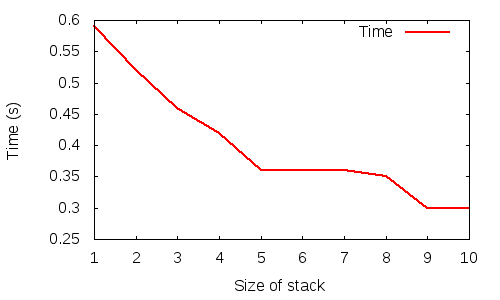
\includegraphics[width=\linewidth]{Shashkova/images/dfs_time.png}}
   \caption{Время работы программы в зависимости от величины стека c алгоритмом Mark (DFS)}
   \label{ris:dtime}   
   \center{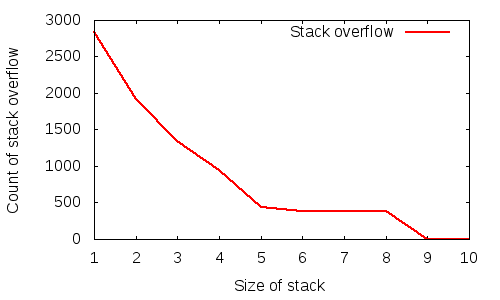
\includegraphics[width=\linewidth]{Shashkova/images/dfs_overflow_count.png}}
   \caption{Количество переполнений стека с алгоритмом Mark (DFS)}  
   \label{ris:dof}
   \end{figure}
   \begin{figure}
   \center{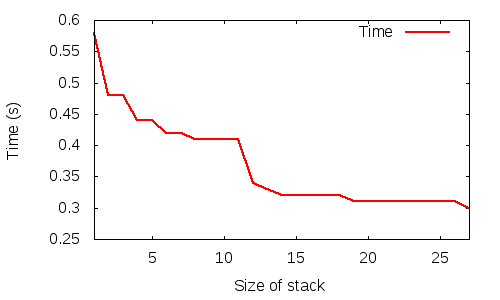
\includegraphics[width=\linewidth]{Shashkova/images/bfs_time.png}}
   \caption{Время работы программы в зависимости от величины стека c алгоритмом Mark (BFS)}
   \label{ris:btime}   
   \center{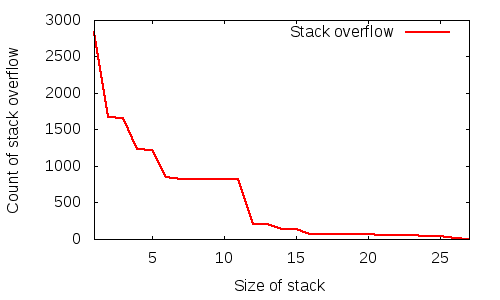
\includegraphics[width=\linewidth]{Shashkova/images/bfs_overflow_count.png}}
   \caption{Количество переполнений стека c алгоритмом Mark (BFS)}
   \label{ris:bof}
   \end{figure}
   

На рис.~\ref{ris:dof} показана зависимость количества переполнений стека от размера стека. Из этого графика хорошо видно, почему график времени работы имеет такую 
неравномерную структуру, а также «ступень». Становится понятно, что время работы программы с переполнениями стека напрямую зависит от количества этих переполнений,
которые происходили в процессе выполнения. И равномерное убывание времени на промежутке от 1 до 5, и постоянное время на промежутке от 5 до 8 полностью объясняется 
зависимостью количества переполнений, которая ведет себя аналогично.

Также были исследованы аналогичные зависимости для алгоритма маркировки с обходом объектов в ширину (Mark (BFS)).

На рис.~\ref{ris:btime} представлена зависимость времени работы программы от величины стека. 
При размере стека, большем 25, переполнения не происходит. Как и в случае с алгоритмом Mark (DFS) в худшем случае (при размере стека $n = 1$) время работы программы
увеличивается почти вдвое. Из особенностей графика можно отметить резкое падение времени работы при увеличении размера стека с 11 до 12. Аналогично для объяснения 
такой зависимости, рассмотрим поведение количества переполнений в зависимости от размера стека.

На рис.~\ref{ris:bof} показана зависимость количества переполнений стека от размера стека с алгоритмом Mark (BFS). Как и в случае с алгоритмом Mark (DFS), очевидно, 
что время работы напрямую зависит от количества происходящих переполнений стека. Резкое падение при изменении размера стека с 11 на 12 также объясняется количеством 
переполнений.

Объясним неравномерность количества переполнений, происходящих при работе каждого из алгоритмов. Будем называть {\it стековой глубиной } корневого объекта максимальную заполненность стека при обходе потомков данного 
корневого объекта.

На графиках рис.~\ref{ris:dm} и рис.~\ref{ris:bm} показано количество корневых объектов в зависимости от их стековой глубины для обоих алгоритмов. 
Из графика рис.~\ref{ris:dm} понятно поведение количества переполнений с алгоритмом Mark (DFS). Количество корневых 
объктов со стековой глубиной от 1 до 5 равномерно убывает, как и убывает количество переполнений. «Ступень» в количестве переполнений также связана с тем, 
что количество корневых объектов стековой глубины больше 5 очень мало по сравнению с объектами меньшей глубины. Поэтому количество переполнений почти не изменяется и 
убывает, только когда переполнения перестают возникать вовсе.

Аналогично для алгоритма Mark (BFS) из рис.~\ref{ris:bm} видно, что количество корневых объектов со стековой глубиной от 8 до 11 и больше 14 мало по сравнению с другими 
объектами, чем и объясняются постоянные промежутки на графике количества переполнений (рис.~\ref{ris:bof}).

   \begin{figure}[p!]   
   \center{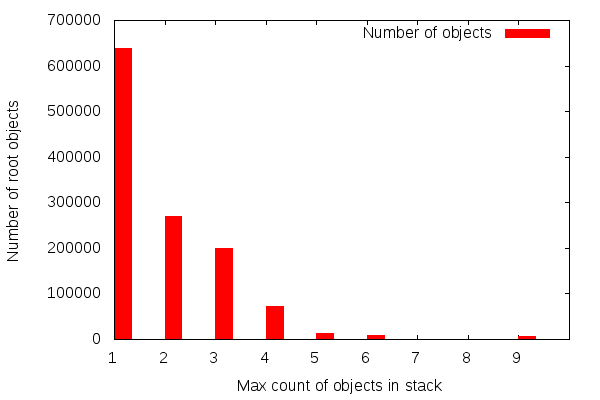
\includegraphics[width=\linewidth]{Shashkova/images/dfs_max_stack.png}}
   \caption{Количество корневых объектов в зависимости от глубины стека с алгоритмом Mark (DFS)}
   \label{ris:dm}   
   \center{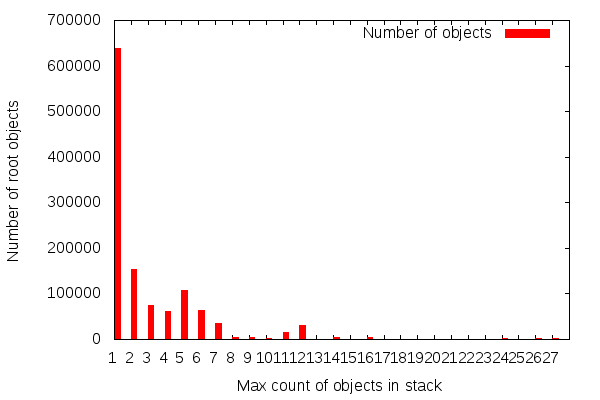
\includegraphics[width=\linewidth]{Shashkova/images/bfs_max_stack.png}}
   \caption{Количество корневых объектов в зависимости от глубины стека с алгоритмом Mark (BFS)}
   \label{ris:bm}   
   \end{figure}


Стоит обратить отдельное внимание на величину стека, при которой происходят переполнения в обоих алгоритмах. Как говорилось ранее, с использованием алгоритма
Mark (BFS) стек перестает переполнятся при размере, большем 9. С алгоритмом Mark (DFS) переполнения происходят вплоть до размера, равного 25. То есть при переходе 
к другому алгоритму размер стека увеличивается почти в 3 раза. Скорее всего, это связано со структурой объектов в тестовой программе. 

Граф, описывающий структуру наших объектов, является лесом из почти деревьев. Под почти деревьями будем понимать традиционные деревья, определенные в теории графов, 
с тем лишь 
отличием, что они могут содержать петли (вершины, связанные ребром сами с собой). Появление петель связано с наличием замыканий (closure) в множестве наших 
объектов. Однако наличие петель не влияет на глубину и ширину дерева, поэтому мы можем считать наши графы деревьями.

Такая значительная разница в размерах стека означает, что у многих деревьев их ширина больше глубины. Анализ объектов в тестовой программе показал, что 
количество потомков у объекта не превышает трех. Даже при небольшой глубине дерева количество объектов на каждом уровне растет довольно быстро, что и приводит 
к увеличению размера используемого стека при обходе в ширину, в отличие от обхода в глубину.

\section*{Заключение}

В результате работы была проведена интеграция бэкенда для языка OCaml и расширения для сборки мусора в LLVM. Было изучено внутреннее 
представление объектов в языке OCaml и реализованы два итеративных алгоритма обхода объектов в стадии пометки сборщика мусора. Результат работы был протестирован
на простейших программах и корректно работает на более сложных примерах. 

\begin{thebibliography}{99}
\bibitem{LLVM} Chris Lattner.
LLVM: An Infrastructure for Multi-Stage Optimization.
Computer Science Dept., University of Illinois at Urbana-Champaign, 2002.

\bibitem{samofal}
Самофалов А.В. Принципы организации сборщика мусора в инфраструктуре LLVM // 
Настоящий сборник.

\bibitem{knuth}
Д. Кнут. Искусство программирования, том 1. Основные алгоритмы.
М.: ``Вильямс»'', 2006.

\bibitem{pliss}
Плисс О.А. Материалы к летней школе ``Управление памятью''. СПбГУ, 2013.

\end{thebibliography}

\title{Сборщик мусора\\
для языка Objective Caml\\
в инфраструктуре LLVM}
%
\titlerunning{Сборщик мусора для языка Objective Caml}
\author{Шашкова Елизавета Михайловна}
%
\authorrunning{Е.М.Шашкова} % abbreviated author list (for running head)
%
%%%% list of authors for the TOC (use if author list has to be modified)
\tocauthor{Е.М.Шашкова}
%
\institute{Санкт-Петербургский государственный университет\\
\email{Elizabeth.Shashkova@gmail.com}}

\maketitle              % typeset the title of the contribution

\section*{Введение}

Сборка мусора --- одна из форм автоматического управления памятью. Специальный компонент поддержки среды времени исполнения, 
называемый сборщиком мусора, автоматически освобождает 
память, удаляя объекты, которые больше не являются доступными для использования.  Сборка мусора освобождает программиста от 
необходимости вручную выделять и освобождать память и позволяет сконцентрироваться на выполнении других задач.
В большинстве современных языков все чаще происходит отказ от предоставления явных средств управления памятью в пользу сборки мусора.

Сборка мусора тесно связана с реализацией компилятора: например, он должен предоставлять сборщику мусора способ определить адреса корневых объектов во
время исполнения. Один из основных
подходов к созданию компиляторов --- использование инфраструктур. Одной из таких инфраструктур построения компиляторов является LLVM 
(Low Level Virtual Machine)~\cite{LLVM}. 

LLVM предназначена 
для анализа, трансформации и оптимизации программ. В основе LLVM лежит промежуточное представление кода 
(Intermediate Representation, IR), над которым можно производить трансформации во время компиляции и компоновки. 
Из этого представления генерируется оптимизированный машинный код для целого ряда платформ.

Objective Caml (OCaml)\footnote{www.caml.inria.fr} --- современный объектно-ориентированный язык функционального программирования общего назначения.
Для языка OCaml существует единственный компилятор от разработчиков самого языка, однако он содержит довольно много платформозависимого кода.
LLVM улучшает переносимость кода между различными платформами и тем самым упрощает процесс построения 
собственного компилятора. Однако язык OCaml требует сборки мусора и реализованный для него бэкенд рассчитывает на наличие сборщика мусора. Но в 
инфраструктуре LLVM нет стандартного способа осуществления сборки мусора, и разработчики предоставили 
возможность для создания расширения LLVM, позволяющего её реализовывать. Данное расширение было реализовано в виде подключаемого модуля~\cite{samofal}.

Целью данной курсовой работы является проведение интеграции бэкенда для языка OCaml и расширения для сборки мусора в LLVM. Необходимо изучить внутреннее 
устройство объектов в языке OCaml и реализвать стадию пометки (mark) для алгоритма сборки мусора mark-and-sweep.

\section{Представление данных в OCaml}

Стадия пометки в алгоритме сборки мусора mark-and-sweep заключается в том, чтобы обойти все "живые" (всё ещё доступные из корневого множества)
объекты и пометить их. Затем на стадии очистки все объекты, которые не были помечены на данной стадии, будут считаться недоступными в программе, а значит,
будут подлежать удалению.

Для реализации стадии пометки необходимо узнать внутреннее устройство объектов.
Все значения в языке OCaml имеют единообразное представление: все они являются типом value языка C (это значение и макросы для работы с ним
определены в файле caml/mlvalues.h). Объект типа value может являться:

\begin{itemize}
   \item целым числом;
   \item указателем на блок внутри кучи;
   \item указателем на блоки вне кучи.
\end{itemize}

Целые числа находятся не в куче, поэтому сборщиком мусора рассматриваться не будут. Блоки, находящиеся в куче, являются основной целью работы сборщика
мусора. Каждый блок содержит заголовок с информацией о длине блока и теге.

Тег определяет структуру блока. Теги со значением меньше, чем \texttt{No\_scan\_tag}, 
означают, что данный блок является корректно структурированным и может быть рекурсивно обойден сборщиком мусора. 
Теги со значением больше, либо равные \texttt{No\_scan\_tag}, означают, что содержимое данного блока должно быть проигнорировано сборщиком мусора. 
Соответствие внутреннего содержимого блоков их тегам показано на рис.~\ref{block_types}.

\begin{figure}[t]
    \begin{tabular}{|l| p{6cm}|}
    \hline
    Тег & Содержимое блока \\
    \hline
    от 0 до \texttt{No\_scan\_tag} -- 1 & Структурированный блок (массив объектов OCaml). Каждое поле является типом value.\\
    \hline
    \texttt{Closure\_tag} & Замыкание представляет собой функциональное значение. Первое слово является указателем на участок кода,
    остальные являются объектами типа value.\\
    \hline
    \texttt{String\_tag} & Строка символов. \\
    \hline
    \texttt{Double\_tag} & Число с плавающей точкой двойной точности. \\
    \hline
    \texttt{Double\_array\_tag} & Массив чисел c плавающей точкой двойной точности. \\
    \hline
    \texttt{Abstract\_tag} & Блок, представляющий абстрактный тип данных. \\
    \hline
    \texttt{Custom\_tag} & Блок, представляющий абстрактный тип данных
    с ``привязанными'' пользовательскими функциями. \\
    \hline
    \end{tabular}
    \caption{Типы блоков в OCaml}
    \label{block_types}
\end{figure}

Благодаря такому устройству объектов становится возможным обход объектов, доступных из живых объектов. Можно быть уверенными,
что в процессе обхода мы не уйдем в область памяти, неинтересную сборщику мусора, а также не пропустим интересующие нас объекты. 

\section{Обход объектов}

Наиболее естественным алгоритмом обхода объектов можно назвать рекурсивный алгоритм. Его описание представлено ниже.
\begin{enumerate}
   \item Алгоритм запускается для каждого корневого объекта.
   \item Проверить, что текущий объект является блоком (а, например, не целым числом).
   \item Если объект является блоком, узнать значение его тега.
   \item Если значение тега меньше значения \texttt{No\_scan\_tag}, объект является живым. Нужно проверить, что
   данный объект находится в куче и пометить его как живой.
   \item Если значение тега больше или равно значению \texttt{No\_scan\_tag}, значит, объект должен игнорироваться сборщиком 
   мусора.
   \item После пометки самого объекта нужно последовательно обойти блоки, содержащиеся внутри данного блока 
   (их количество известно из заголовка) и повторить с ними ту же операцию.
   \item Отдельное внимание нужно уделить объекту с тегом \texttt{Closure\_tag}, так как первое слово является 
   указателем на код и при обходе сборщиком мусора должно игнорироваться.
\end{enumerate}

Однако, рекурсивный вызов функций потребует дополнительной памяти для сохранения стека вызовов, причем размер этого стека предсказать невозможно. Поэтому данный 
алгоритм необходимо было превратить в нерекурсивный, с использованием собственного стека. Структуру объектов программы можно представить в виде графа, где 
вершины --- объекты, а ребра --- ссылки между объектами. Граф можно обойти двумя способами: в ширину (Breadth-first search) и в глубину(Depth-first search).

При обходе в глубину у каждого объекта поочередно просматриваются объекты, на которые он ссылается. Для каждого такого объекта помечаются все его потомки и только 
потом алгоритм переходит к следующему потомку текущего объекта. Код Mark описывает данный алгоритм. Здесь $push()$ и $pop()$ --- операции работы со стеком.

\begin{algorithm}[p]
\caption{Mark}
\label{BFS}
\begin{algorithmic}[1]
    \For {$root \in root\_objects$}
        \If {$is\_object(root)$}
            \If {$tag(root) < No\_scan\_tag$ }
                \If {$root$ in heap}
                    \State {$mark(root)$}
                \EndIf
                \State $push(root)$
                \While {$object \leftarrow pop()$}
                    \State $size \leftarrow size(object)$
                    \If {$tag(object) = Closure\_tag$}
                        \State $i = 1$
                    \Else
                        \State $i = 0$
                    \EndIf
                    \For {$i < size$}
                        \State $child \leftarrow Field(object, i)$
                        \If {   $is\_object(child)$ and\\
                                \hskip\algorithmicindent
                                \hskip\algorithmicindent
                                \hskip\algorithmicindent
                                \hskip\algorithmicindent
                                \hskip\algorithmicindent
                                \hskip\algorithmicindent $tag(child) < No\_scan\_tag$                           
                             }
                            \If {$child$ in heap and not $marked(child)$}
                                \State {$mark(child)$}
                                \State {$push(child)$}
                            \EndIf
                        \EndIf
                    \EndFor
                \EndWhile
            \EndIf
        \EndIf
    \EndFor
    %\EndProcedure
\end{algorithmic}
\end{algorithm}


При обходе в ширину объекты рассматриваются в порядке возрастания расстояния от них до коневого объекта в графе объектов. Данный алгоритм описывается
так же, как и алгоритм Mark, с тем лишь отличием, что вместо стека используется очередь, реализованная на массиве. То есть в данном псевдокоде операции 
$push()$ и $pop()$ --- операции работы с очередью.

Обе модификации данного алгоритма (с обходом в глубину и в ширину) были реализованы итеративно с созданием стека в статической области памяти. 
Отсюда понятно, что размер стека в таком случае является постоянным, и может произойти переполнение стека. Для данной ситуации существует 
специальный алгоритм восстановления.

В случае переполнения стека нельзя допустить некорректную работу сборщика мусора. Если произойдет ошибка в работе стадии пометки, часть живых 
объектов не будут помечены, то есть будут считаться мертвыми и память из-под них будет преждевременно освобождена, что приведет к 
некорректной работе программы. Алгоритм восстановления при переполнении стека был описан в ~\cite{knuth}. Для реализации было решено использовать модификацию 
этого алгоритма~\cite{pliss}. Этот алгоритм, работающий с ограниченной памятью, можно описать следующим образом:

\begin{enumerate}
   \item При заполнении стека алгоритм пометки продолжает свою работу. Однако новые объекты, которые не поместились в стек, в него не добавляются,
   а просто игнорируются.
   \item При переполнении устанавливается специальный флаг, сообщающий о том, что переполнение произошло.
   \item При завершении стадии пометки проверяется состояние флага о переполнении.
   \item Если переполнение произошло, значит, часть живых объектов не была помечена. Начинается последовательный обход кучи.
   \item Флаг переполнения сбрасывается. Начиная с каждого помеченного (то есть точно живого) объекта кучи запускается алгоритм пометки.
   \item Теперь для пометки будет рассматриваться меньше объектов и велика вероятность, что они поместятся в стек. В случае же, если переполнение 
   произойдет снова, алгоритм повторится (снова установится флаг переполнения и т.д.).
\end{enumerate}

Нужно пояснить, что данный алгоритм не будет работать бесконечно долго, так как при каждом последующем запуске стадии пометки мы помечаем 
как минимум $n + 1$ объект из ранее не помеченных (где $n$ --- размер стека). Количество объектов в куче конечно, а значит, процесс когда-нибудь 
закончится. Все живые объекты будут помечены и стадия маркировки корректно выполнит свою задачу даже при условии переполнения стека.

\section{Результаты}
В результате был создан модуль, реализующий стадию маркировки для алгоритма сборки мусора и произведена модификация кучи для обработки переполнения стека.
Реализация была выполнена на языке C. 

Наиболее интересным было исследовать работу программы при переполнении стека. В качестве тестовой программы был взят парсер c С-подобного языка,
написанный на языке OCaml. Он принимает на вход файл для разбора и анализирует его. Во всех экспериментах, представленных ниже, на вход подавался
один и тот же файл. 

Сборка мусора вызывалась автоматически, использовался алгоритм инициализации, основанный на количестве доступной свободной памяти. Согласно 
этому алгоритму, сборка мусора начинается, когда объем занятой памяти в куче превышает некоторый порог, заданный переменной $Threshold$. В данных 
экспериментах значение переменной $Threshold$ равнялось 0.75, что соответствует моментам, когда 75\% объема памяти кучи заняты.  

Благодаря тому, что вызов сборки мусора основывался на количестве доступной памяти, во всех экспериментах количество вызовов сборки мусора было одинаково и равнялось 
1370. К тому же сборка мусора производилась на одинаковых стадиях работы программы.

На рис.~\ref{ris:dtime} представлена зависимость времени работы программы от
величины стека. При размере стека, большем 8, переполнения не происходит. Из графика видно, что переполнение стека значительно, почти в 2 раза, увеличивает 
время работы программы. Из графика видно, что время работы равномерно убывает при изменении размера стека от 1 до 5. При дальнейшем увеличении размера стека, 
на графике заметна некоторая «ступень»: при увеличении размера стека от 5 до 8 время работы программы почти не изменяется. И лишь после этого оно еще раз уменьшается 
и перестает зависеть от дальнейшего увеличения стека. 

Для исследования такого поведения, исследуем количество переполнений, происходящих при работе программы.

   \begin{figure}[p]   
   \center{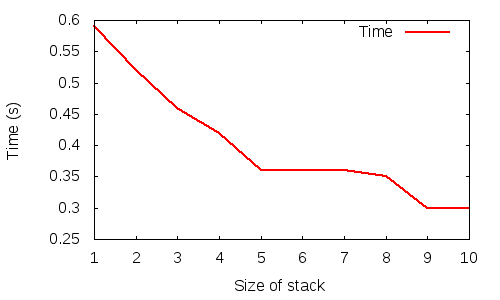
\includegraphics[width=\linewidth]{Shashkova/images/dfs_time.png}}
   \caption{Время работы программы в зависимости от величины стека c алгоритмом Mark (DFS)}
   \label{ris:dtime}   
   \center{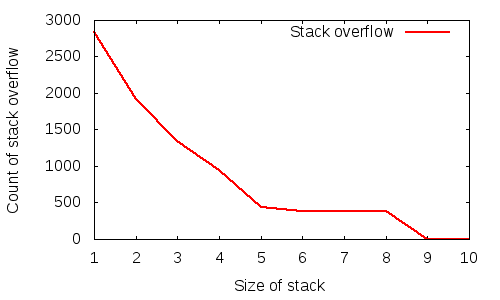
\includegraphics[width=\linewidth]{Shashkova/images/dfs_overflow_count.png}}
   \caption{Количество переполнений стека с алгоритмом Mark (DFS)}  
   \label{ris:dof}
   \end{figure}
   \begin{figure}
   \center{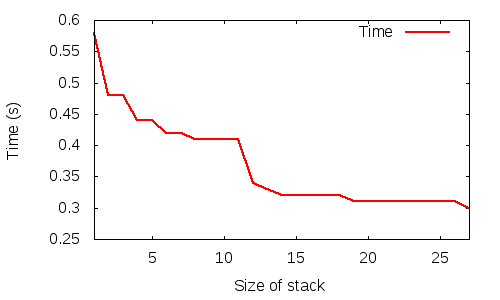
\includegraphics[width=\linewidth]{Shashkova/images/bfs_time.png}}
   \caption{Время работы программы в зависимости от величины стека c алгоритмом Mark (BFS)}
   \label{ris:btime}   
   \center{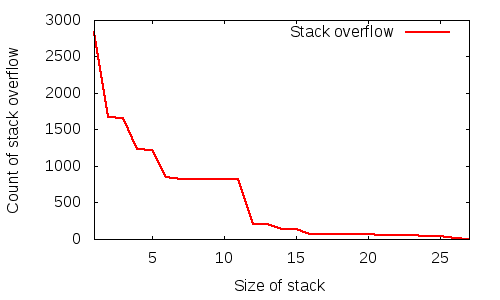
\includegraphics[width=\linewidth]{Shashkova/images/bfs_overflow_count.png}}
   \caption{Количество переполнений стека c алгоритмом Mark (BFS)}
   \label{ris:bof}
   \end{figure}
   

На рис.~\ref{ris:dof} показана зависимость количества переполнений стека от размера стека. Из этого графика хорошо видно, почему график времени работы имеет такую 
неравномерную структуру, а также «ступень». Становится понятно, что время работы программы с переполнениями стека напрямую зависит от количества этих переполнений,
которые происходили в процессе выполнения. И равномерное убывание времени на промежутке от 1 до 5, и постоянное время на промежутке от 5 до 8 полностью объясняется 
зависимостью количества переполнений, которая ведет себя аналогично.

Также были исследованы аналогичные зависимости для алгоритма маркировки с обходом объектов в ширину (Mark (BFS)).

На рис.~\ref{ris:btime} представлена зависимость времени работы программы от величины стека. 
При размере стека, большем 25, переполнения не происходит. Как и в случае с алгоритмом Mark (DFS) в худшем случае (при размере стека $n = 1$) время работы программы
увеличивается почти вдвое. Из особенностей графика можно отметить резкое падение времени работы при увеличении размера стека с 11 до 12. Аналогично для объяснения 
такой зависимости, рассмотрим поведение количества переполнений в зависимости от размера стека.

На рис.~\ref{ris:bof} показана зависимость количества переполнений стека от размера стека с алгоритмом Mark (BFS). Как и в случае с алгоритмом Mark (DFS), очевидно, 
что время работы напрямую зависит от количества происходящих переполнений стека. Резкое падение при изменении размера стека с 11 на 12 также объясняется количеством 
переполнений.

Объясним неравномерность количества переполнений, происходящих при работе каждого из алгоритмов. Будем называть {\it стековой глубиной } корневого объекта максимальную заполненность стека при обходе потомков данного 
корневого объекта.

На графиках рис.~\ref{ris:dm} и рис.~\ref{ris:bm} показано количество корневых объектов в зависимости от их стековой глубины для обоих алгоритмов. 
Из графика рис.~\ref{ris:dm} понятно поведение количества переполнений с алгоритмом Mark (DFS). Количество корневых 
объктов со стековой глубиной от 1 до 5 равномерно убывает, как и убывает количество переполнений. «Ступень» в количестве переполнений также связана с тем, 
что количество корневых объектов стековой глубины больше 5 очень мало по сравнению с объектами меньшей глубины. Поэтому количество переполнений почти не изменяется и 
убывает, только когда переполнения перестают возникать вовсе.

Аналогично для алгоритма Mark (BFS) из рис.~\ref{ris:bm} видно, что количество корневых объектов со стековой глубиной от 8 до 11 и больше 14 мало по сравнению с другими 
объектами, чем и объясняются постоянные промежутки на графике количества переполнений (рис.~\ref{ris:bof}).

   \begin{figure}[p!]   
   \center{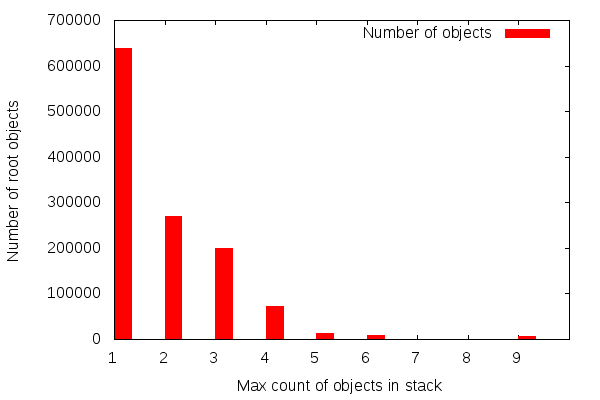
\includegraphics[width=\linewidth]{Shashkova/images/dfs_max_stack.png}}
   \caption{Количество корневых объектов в зависимости от глубины стека с алгоритмом Mark (DFS)}
   \label{ris:dm}   
   \center{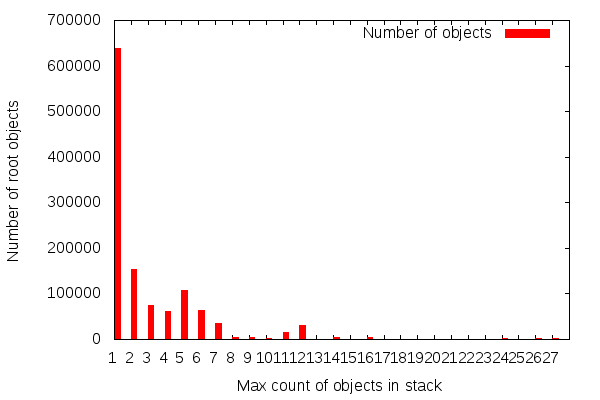
\includegraphics[width=\linewidth]{Shashkova/images/bfs_max_stack.png}}
   \caption{Количество корневых объектов в зависимости от глубины стека с алгоритмом Mark (BFS)}
   \label{ris:bm}   
   \end{figure}


Стоит обратить отдельное внимание на величину стека, при которой происходят переполнения в обоих алгоритмах. Как говорилось ранее, с использованием алгоритма
Mark (BFS) стек перестает переполнятся при размере, большем 9. С алгоритмом Mark (DFS) переполнения происходят вплоть до размера, равного 25. То есть при переходе 
к другому алгоритму размер стека увеличивается почти в 3 раза. Скорее всего, это связано со структурой объектов в тестовой программе. 

Граф, описывающий структуру наших объектов, является лесом из почти деревьев. Под почти деревьями будем понимать традиционные деревья, определенные в теории графов, 
с тем лишь 
отличием, что они могут содержать петли (вершины, связанные ребром сами с собой). Появление петель связано с наличием замыканий (closure) в множестве наших 
объектов. Однако наличие петель не влияет на глубину и ширину дерева, поэтому мы можем считать наши графы деревьями.

Такая значительная разница в размерах стека означает, что у многих деревьев их ширина больше глубины. Анализ объектов в тестовой программе показал, что 
количество потомков у объекта не превышает трех. Даже при небольшой глубине дерева количество объектов на каждом уровне растет довольно быстро, что и приводит 
к увеличению размера используемого стека при обходе в ширину, в отличие от обхода в глубину.

\section*{Заключение}

В результате работы была проведена интеграция бэкенда для языка OCaml и расширения для сборки мусора в LLVM. Было изучено внутреннее 
представление объектов в языке OCaml и реализованы два итеративных алгоритма обхода объектов в стадии пометки сборщика мусора. Результат работы был протестирован
на простейших программах и корректно работает на более сложных примерах. 

\begin{thebibliography}{99}
\bibitem{LLVM} Chris Lattner.
LLVM: An Infrastructure for Multi-Stage Optimization.
Computer Science Dept., University of Illinois at Urbana-Champaign, 2002.

\bibitem{samofal}
Самофалов А.В. Принципы организации сборщика мусора в инфраструктуре LLVM // 
Настоящий сборник.

\bibitem{knuth}
Д. Кнут. Искусство программирования, том 1. Основные алгоритмы.
М.: ``Вильямс»'', 2006.

\bibitem{pliss}
Плисс О.А. Материалы к летней школе ``Управление памятью''. СПбГУ, 2013.

\end{thebibliography}

\title{Сборщик мусора\\
для языка Objective Caml\\
в инфраструктуре LLVM}
%
\titlerunning{Сборщик мусора для языка Objective Caml}
\author{Шашкова Елизавета Михайловна}
%
\authorrunning{Е.М.Шашкова} % abbreviated author list (for running head)
%
%%%% list of authors for the TOC (use if author list has to be modified)
\tocauthor{Е.М.Шашкова}
%
\institute{Санкт-Петербургский государственный университет\\
\email{Elizabeth.Shashkova@gmail.com}}

\maketitle              % typeset the title of the contribution

\section*{Введение}

Сборка мусора --- одна из форм автоматического управления памятью. Специальный компонент поддержки среды времени исполнения, 
называемый сборщиком мусора, автоматически освобождает 
память, удаляя объекты, которые больше не являются доступными для использования.  Сборка мусора освобождает программиста от 
необходимости вручную выделять и освобождать память и позволяет сконцентрироваться на выполнении других задач.
В большинстве современных языков все чаще происходит отказ от предоставления явных средств управления памятью в пользу сборки мусора.

Сборка мусора тесно связана с реализацией компилятора: например, он должен предоставлять сборщику мусора способ определить адреса корневых объектов во
время исполнения. Один из основных
подходов к созданию компиляторов --- использование инфраструктур. Одной из таких инфраструктур построения компиляторов является LLVM 
(Low Level Virtual Machine)~\cite{LLVM}. 

LLVM предназначена 
для анализа, трансформации и оптимизации программ. В основе LLVM лежит промежуточное представление кода 
(Intermediate Representation, IR), над которым можно производить трансформации во время компиляции и компоновки. 
Из этого представления генерируется оптимизированный машинный код для целого ряда платформ.

Objective Caml (OCaml)\footnote{www.caml.inria.fr} --- современный объектно-ориентированный язык функционального программирования общего назначения.
Для языка OCaml существует единственный компилятор от разработчиков самого языка, однако он содержит довольно много платформозависимого кода.
LLVM улучшает переносимость кода между различными платформами и тем самым упрощает процесс построения 
собственного компилятора. Однако язык OCaml требует сборки мусора и реализованный для него бэкенд рассчитывает на наличие сборщика мусора. Но в 
инфраструктуре LLVM нет стандартного способа осуществления сборки мусора, и разработчики предоставили 
возможность для создания расширения LLVM, позволяющего её реализовывать. Данное расширение было реализовано в виде подключаемого модуля~\cite{samofal}.

Целью данной курсовой работы является проведение интеграции бэкенда для языка OCaml и расширения для сборки мусора в LLVM. Необходимо изучить внутреннее 
устройство объектов в языке OCaml и реализвать стадию пометки (mark) для алгоритма сборки мусора mark-and-sweep.

\section{Представление данных в OCaml}

Стадия пометки в алгоритме сборки мусора mark-and-sweep заключается в том, чтобы обойти все "живые" (всё ещё доступные из корневого множества)
объекты и пометить их. Затем на стадии очистки все объекты, которые не были помечены на данной стадии, будут считаться недоступными в программе, а значит,
будут подлежать удалению.

Для реализации стадии пометки необходимо узнать внутреннее устройство объектов.
Все значения в языке OCaml имеют единообразное представление: все они являются типом value языка C (это значение и макросы для работы с ним
определены в файле caml/mlvalues.h). Объект типа value может являться:

\begin{itemize}
   \item целым числом;
   \item указателем на блок внутри кучи;
   \item указателем на блоки вне кучи.
\end{itemize}

Целые числа находятся не в куче, поэтому сборщиком мусора рассматриваться не будут. Блоки, находящиеся в куче, являются основной целью работы сборщика
мусора. Каждый блок содержит заголовок с информацией о длине блока и теге.

Тег определяет структуру блока. Теги со значением меньше, чем \texttt{No\_scan\_tag}, 
означают, что данный блок является корректно структурированным и может быть рекурсивно обойден сборщиком мусора. 
Теги со значением больше, либо равные \texttt{No\_scan\_tag}, означают, что содержимое данного блока должно быть проигнорировано сборщиком мусора. 
Соответствие внутреннего содержимого блоков их тегам показано на рис.~\ref{block_types}.

\begin{figure}[t]
    \begin{tabular}{|l| p{6cm}|}
    \hline
    Тег & Содержимое блока \\
    \hline
    от 0 до \texttt{No\_scan\_tag} -- 1 & Структурированный блок (массив объектов OCaml). Каждое поле является типом value.\\
    \hline
    \texttt{Closure\_tag} & Замыкание представляет собой функциональное значение. Первое слово является указателем на участок кода,
    остальные являются объектами типа value.\\
    \hline
    \texttt{String\_tag} & Строка символов. \\
    \hline
    \texttt{Double\_tag} & Число с плавающей точкой двойной точности. \\
    \hline
    \texttt{Double\_array\_tag} & Массив чисел c плавающей точкой двойной точности. \\
    \hline
    \texttt{Abstract\_tag} & Блок, представляющий абстрактный тип данных. \\
    \hline
    \texttt{Custom\_tag} & Блок, представляющий абстрактный тип данных
    с ``привязанными'' пользовательскими функциями. \\
    \hline
    \end{tabular}
    \caption{Типы блоков в OCaml}
    \label{block_types}
\end{figure}

Благодаря такому устройству объектов становится возможным обход объектов, доступных из живых объектов. Можно быть уверенными,
что в процессе обхода мы не уйдем в область памяти, неинтересную сборщику мусора, а также не пропустим интересующие нас объекты. 

\section{Обход объектов}

Наиболее естественным алгоритмом обхода объектов можно назвать рекурсивный алгоритм. Его описание представлено ниже.
\begin{enumerate}
   \item Алгоритм запускается для каждого корневого объекта.
   \item Проверить, что текущий объект является блоком (а, например, не целым числом).
   \item Если объект является блоком, узнать значение его тега.
   \item Если значение тега меньше значения \texttt{No\_scan\_tag}, объект является живым. Нужно проверить, что
   данный объект находится в куче и пометить его как живой.
   \item Если значение тега больше или равно значению \texttt{No\_scan\_tag}, значит, объект должен игнорироваться сборщиком 
   мусора.
   \item После пометки самого объекта нужно последовательно обойти блоки, содержащиеся внутри данного блока 
   (их количество известно из заголовка) и повторить с ними ту же операцию.
   \item Отдельное внимание нужно уделить объекту с тегом \texttt{Closure\_tag}, так как первое слово является 
   указателем на код и при обходе сборщиком мусора должно игнорироваться.
\end{enumerate}

Однако, рекурсивный вызов функций потребует дополнительной памяти для сохранения стека вызовов, причем размер этого стека предсказать невозможно. Поэтому данный 
алгоритм необходимо было превратить в нерекурсивный, с использованием собственного стека. Структуру объектов программы можно представить в виде графа, где 
вершины --- объекты, а ребра --- ссылки между объектами. Граф можно обойти двумя способами: в ширину (Breadth-first search) и в глубину(Depth-first search).

При обходе в глубину у каждого объекта поочередно просматриваются объекты, на которые он ссылается. Для каждого такого объекта помечаются все его потомки и только 
потом алгоритм переходит к следующему потомку текущего объекта. Код Mark описывает данный алгоритм. Здесь $push()$ и $pop()$ --- операции работы со стеком.

\begin{algorithm}[p]
\caption{Mark}
\label{BFS}
\begin{algorithmic}[1]
    \For {$root \in root\_objects$}
        \If {$is\_object(root)$}
            \If {$tag(root) < No\_scan\_tag$ }
                \If {$root$ in heap}
                    \State {$mark(root)$}
                \EndIf
                \State $push(root)$
                \While {$object \leftarrow pop()$}
                    \State $size \leftarrow size(object)$
                    \If {$tag(object) = Closure\_tag$}
                        \State $i = 1$
                    \Else
                        \State $i = 0$
                    \EndIf
                    \For {$i < size$}
                        \State $child \leftarrow Field(object, i)$
                        \If {   $is\_object(child)$ and\\
                                \hskip\algorithmicindent
                                \hskip\algorithmicindent
                                \hskip\algorithmicindent
                                \hskip\algorithmicindent
                                \hskip\algorithmicindent
                                \hskip\algorithmicindent $tag(child) < No\_scan\_tag$                           
                             }
                            \If {$child$ in heap and not $marked(child)$}
                                \State {$mark(child)$}
                                \State {$push(child)$}
                            \EndIf
                        \EndIf
                    \EndFor
                \EndWhile
            \EndIf
        \EndIf
    \EndFor
    %\EndProcedure
\end{algorithmic}
\end{algorithm}


При обходе в ширину объекты рассматриваются в порядке возрастания расстояния от них до коневого объекта в графе объектов. Данный алгоритм описывается
так же, как и алгоритм Mark, с тем лишь отличием, что вместо стека используется очередь, реализованная на массиве. То есть в данном псевдокоде операции 
$push()$ и $pop()$ --- операции работы с очередью.

Обе модификации данного алгоритма (с обходом в глубину и в ширину) были реализованы итеративно с созданием стека в статической области памяти. 
Отсюда понятно, что размер стека в таком случае является постоянным, и может произойти переполнение стека. Для данной ситуации существует 
специальный алгоритм восстановления.

В случае переполнения стека нельзя допустить некорректную работу сборщика мусора. Если произойдет ошибка в работе стадии пометки, часть живых 
объектов не будут помечены, то есть будут считаться мертвыми и память из-под них будет преждевременно освобождена, что приведет к 
некорректной работе программы. Алгоритм восстановления при переполнении стека был описан в ~\cite{knuth}. Для реализации было решено использовать модификацию 
этого алгоритма~\cite{pliss}. Этот алгоритм, работающий с ограниченной памятью, можно описать следующим образом:

\begin{enumerate}
   \item При заполнении стека алгоритм пометки продолжает свою работу. Однако новые объекты, которые не поместились в стек, в него не добавляются,
   а просто игнорируются.
   \item При переполнении устанавливается специальный флаг, сообщающий о том, что переполнение произошло.
   \item При завершении стадии пометки проверяется состояние флага о переполнении.
   \item Если переполнение произошло, значит, часть живых объектов не была помечена. Начинается последовательный обход кучи.
   \item Флаг переполнения сбрасывается. Начиная с каждого помеченного (то есть точно живого) объекта кучи запускается алгоритм пометки.
   \item Теперь для пометки будет рассматриваться меньше объектов и велика вероятность, что они поместятся в стек. В случае же, если переполнение 
   произойдет снова, алгоритм повторится (снова установится флаг переполнения и т.д.).
\end{enumerate}

Нужно пояснить, что данный алгоритм не будет работать бесконечно долго, так как при каждом последующем запуске стадии пометки мы помечаем 
как минимум $n + 1$ объект из ранее не помеченных (где $n$ --- размер стека). Количество объектов в куче конечно, а значит, процесс когда-нибудь 
закончится. Все живые объекты будут помечены и стадия маркировки корректно выполнит свою задачу даже при условии переполнения стека.

\section{Результаты}
В результате был создан модуль, реализующий стадию маркировки для алгоритма сборки мусора и произведена модификация кучи для обработки переполнения стека.
Реализация была выполнена на языке C. 

Наиболее интересным было исследовать работу программы при переполнении стека. В качестве тестовой программы был взят парсер c С-подобного языка,
написанный на языке OCaml. Он принимает на вход файл для разбора и анализирует его. Во всех экспериментах, представленных ниже, на вход подавался
один и тот же файл. 

Сборка мусора вызывалась автоматически, использовался алгоритм инициализации, основанный на количестве доступной свободной памяти. Согласно 
этому алгоритму, сборка мусора начинается, когда объем занятой памяти в куче превышает некоторый порог, заданный переменной $Threshold$. В данных 
экспериментах значение переменной $Threshold$ равнялось 0.75, что соответствует моментам, когда 75\% объема памяти кучи заняты.  

Благодаря тому, что вызов сборки мусора основывался на количестве доступной памяти, во всех экспериментах количество вызовов сборки мусора было одинаково и равнялось 
1370. К тому же сборка мусора производилась на одинаковых стадиях работы программы.

На рис.~\ref{ris:dtime} представлена зависимость времени работы программы от
величины стека. При размере стека, большем 8, переполнения не происходит. Из графика видно, что переполнение стека значительно, почти в 2 раза, увеличивает 
время работы программы. Из графика видно, что время работы равномерно убывает при изменении размера стека от 1 до 5. При дальнейшем увеличении размера стека, 
на графике заметна некоторая «ступень»: при увеличении размера стека от 5 до 8 время работы программы почти не изменяется. И лишь после этого оно еще раз уменьшается 
и перестает зависеть от дальнейшего увеличения стека. 

Для исследования такого поведения, исследуем количество переполнений, происходящих при работе программы.

   \begin{figure}[p]   
   \center{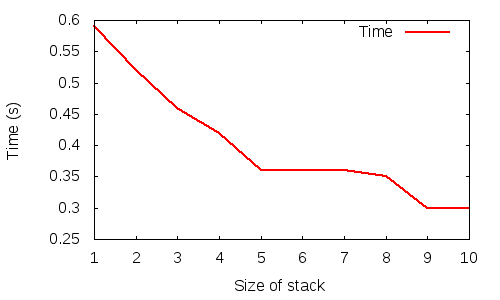
\includegraphics[width=\linewidth]{Shashkova/images/dfs_time.png}}
   \caption{Время работы программы в зависимости от величины стека c алгоритмом Mark (DFS)}
   \label{ris:dtime}   
   \center{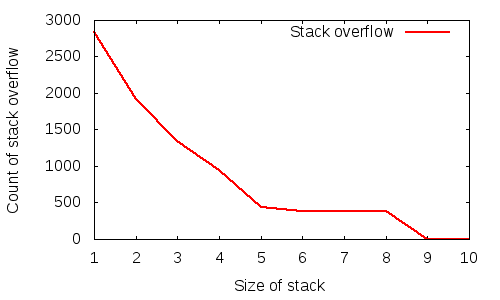
\includegraphics[width=\linewidth]{Shashkova/images/dfs_overflow_count.png}}
   \caption{Количество переполнений стека с алгоритмом Mark (DFS)}  
   \label{ris:dof}
   \end{figure}
   \begin{figure}
   \center{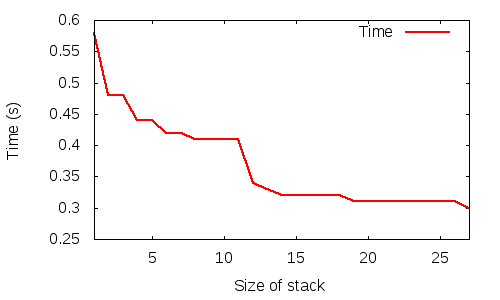
\includegraphics[width=\linewidth]{Shashkova/images/bfs_time.png}}
   \caption{Время работы программы в зависимости от величины стека c алгоритмом Mark (BFS)}
   \label{ris:btime}   
   \center{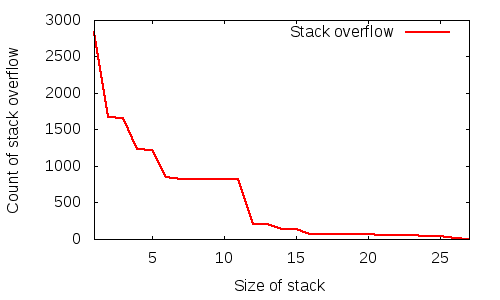
\includegraphics[width=\linewidth]{Shashkova/images/bfs_overflow_count.png}}
   \caption{Количество переполнений стека c алгоритмом Mark (BFS)}
   \label{ris:bof}
   \end{figure}
   

На рис.~\ref{ris:dof} показана зависимость количества переполнений стека от размера стека. Из этого графика хорошо видно, почему график времени работы имеет такую 
неравномерную структуру, а также «ступень». Становится понятно, что время работы программы с переполнениями стека напрямую зависит от количества этих переполнений,
которые происходили в процессе выполнения. И равномерное убывание времени на промежутке от 1 до 5, и постоянное время на промежутке от 5 до 8 полностью объясняется 
зависимостью количества переполнений, которая ведет себя аналогично.

Также были исследованы аналогичные зависимости для алгоритма маркировки с обходом объектов в ширину (Mark (BFS)).

На рис.~\ref{ris:btime} представлена зависимость времени работы программы от величины стека. 
При размере стека, большем 25, переполнения не происходит. Как и в случае с алгоритмом Mark (DFS) в худшем случае (при размере стека $n = 1$) время работы программы
увеличивается почти вдвое. Из особенностей графика можно отметить резкое падение времени работы при увеличении размера стека с 11 до 12. Аналогично для объяснения 
такой зависимости, рассмотрим поведение количества переполнений в зависимости от размера стека.

На рис.~\ref{ris:bof} показана зависимость количества переполнений стека от размера стека с алгоритмом Mark (BFS). Как и в случае с алгоритмом Mark (DFS), очевидно, 
что время работы напрямую зависит от количества происходящих переполнений стека. Резкое падение при изменении размера стека с 11 на 12 также объясняется количеством 
переполнений.

Объясним неравномерность количества переполнений, происходящих при работе каждого из алгоритмов. Будем называть {\it стековой глубиной } корневого объекта максимальную заполненность стека при обходе потомков данного 
корневого объекта.

На графиках рис.~\ref{ris:dm} и рис.~\ref{ris:bm} показано количество корневых объектов в зависимости от их стековой глубины для обоих алгоритмов. 
Из графика рис.~\ref{ris:dm} понятно поведение количества переполнений с алгоритмом Mark (DFS). Количество корневых 
объктов со стековой глубиной от 1 до 5 равномерно убывает, как и убывает количество переполнений. «Ступень» в количестве переполнений также связана с тем, 
что количество корневых объектов стековой глубины больше 5 очень мало по сравнению с объектами меньшей глубины. Поэтому количество переполнений почти не изменяется и 
убывает, только когда переполнения перестают возникать вовсе.

Аналогично для алгоритма Mark (BFS) из рис.~\ref{ris:bm} видно, что количество корневых объектов со стековой глубиной от 8 до 11 и больше 14 мало по сравнению с другими 
объектами, чем и объясняются постоянные промежутки на графике количества переполнений (рис.~\ref{ris:bof}).

   \begin{figure}[p!]   
   \center{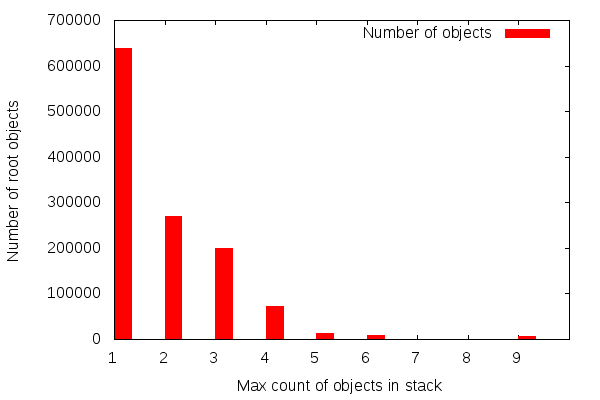
\includegraphics[width=\linewidth]{Shashkova/images/dfs_max_stack.png}}
   \caption{Количество корневых объектов в зависимости от глубины стека с алгоритмом Mark (DFS)}
   \label{ris:dm}   
   \center{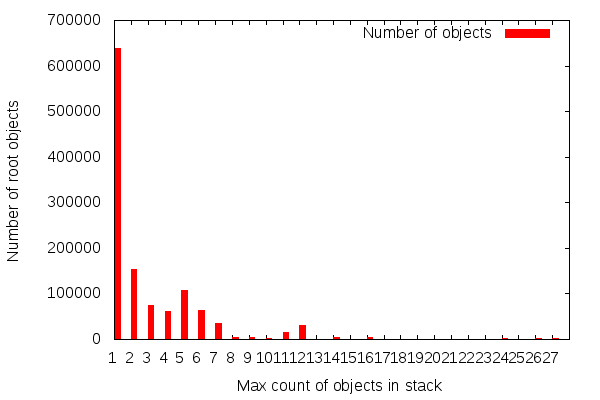
\includegraphics[width=\linewidth]{Shashkova/images/bfs_max_stack.png}}
   \caption{Количество корневых объектов в зависимости от глубины стека с алгоритмом Mark (BFS)}
   \label{ris:bm}   
   \end{figure}


Стоит обратить отдельное внимание на величину стека, при которой происходят переполнения в обоих алгоритмах. Как говорилось ранее, с использованием алгоритма
Mark (BFS) стек перестает переполнятся при размере, большем 9. С алгоритмом Mark (DFS) переполнения происходят вплоть до размера, равного 25. То есть при переходе 
к другому алгоритму размер стека увеличивается почти в 3 раза. Скорее всего, это связано со структурой объектов в тестовой программе. 

Граф, описывающий структуру наших объектов, является лесом из почти деревьев. Под почти деревьями будем понимать традиционные деревья, определенные в теории графов, 
с тем лишь 
отличием, что они могут содержать петли (вершины, связанные ребром сами с собой). Появление петель связано с наличием замыканий (closure) в множестве наших 
объектов. Однако наличие петель не влияет на глубину и ширину дерева, поэтому мы можем считать наши графы деревьями.

Такая значительная разница в размерах стека означает, что у многих деревьев их ширина больше глубины. Анализ объектов в тестовой программе показал, что 
количество потомков у объекта не превышает трех. Даже при небольшой глубине дерева количество объектов на каждом уровне растет довольно быстро, что и приводит 
к увеличению размера используемого стека при обходе в ширину, в отличие от обхода в глубину.

\section*{Заключение}

В результате работы была проведена интеграция бэкенда для языка OCaml и расширения для сборки мусора в LLVM. Было изучено внутреннее 
представление объектов в языке OCaml и реализованы два итеративных алгоритма обхода объектов в стадии пометки сборщика мусора. Результат работы был протестирован
на простейших программах и корректно работает на более сложных примерах. 

\begin{thebibliography}{99}
\bibitem{LLVM} Chris Lattner.
LLVM: An Infrastructure for Multi-Stage Optimization.
Computer Science Dept., University of Illinois at Urbana-Champaign, 2002.

\bibitem{samofal}
Самофалов А.В. Принципы организации сборщика мусора в инфраструктуре LLVM // 
Настоящий сборник.

\bibitem{knuth}
Д. Кнут. Искусство программирования, том 1. Основные алгоритмы.
М.: ``Вильямс»'', 2006.

\bibitem{pliss}
Плисс О.А. Материалы к летней школе ``Управление памятью''. СПбГУ, 2013.

\end{thebibliography}


\title{Сборщик мусора\\
для языка Objective Caml\\
в инфраструктуре LLVM}
%
\titlerunning{Сборщик мусора для языка Objective Caml}
\author{Шашкова Елизавета Михайловна}
%
\authorrunning{Е.М.Шашкова} % abbreviated author list (for running head)
%
%%%% list of authors for the TOC (use if author list has to be modified)
\tocauthor{Е.М.Шашкова}
%
\institute{Санкт-Петербургский государственный университет\\
\email{Elizabeth.Shashkova@gmail.com}}

\maketitle              % typeset the title of the contribution

\section*{Введение}

Сборка мусора --- одна из форм автоматического управления памятью. Специальный компонент поддержки среды времени исполнения, 
называемый сборщиком мусора, автоматически освобождает 
память, удаляя объекты, которые больше не являются доступными для использования.  Сборка мусора освобождает программиста от 
необходимости вручную выделять и освобождать память и позволяет сконцентрироваться на выполнении других задач.
В большинстве современных языков все чаще происходит отказ от предоставления явных средств управления памятью в пользу сборки мусора.

Сборка мусора тесно связана с реализацией компилятора: например, он должен предоставлять сборщику мусора способ определить адреса корневых объектов во
время исполнения. Один из основных
подходов к созданию компиляторов --- использование инфраструктур. Одной из таких инфраструктур построения компиляторов является LLVM 
(Low Level Virtual Machine)~\cite{LLVM}. 

LLVM предназначена 
для анализа, трансформации и оптимизации программ. В основе LLVM лежит промежуточное представление кода 
(Intermediate Representation, IR), над которым можно производить трансформации во время компиляции и компоновки. 
Из этого представления генерируется оптимизированный машинный код для целого ряда платформ.

Objective Caml (OCaml)\footnote{www.caml.inria.fr} --- современный объектно-ориентированный язык функционального программирования общего назначения.
Для языка OCaml существует единственный компилятор от разработчиков самого языка, однако он содержит довольно много платформозависимого кода.
LLVM улучшает переносимость кода между различными платформами и тем самым упрощает процесс построения 
собственного компилятора. Однако язык OCaml требует сборки мусора и реализованный для него бэкенд рассчитывает на наличие сборщика мусора. Но в 
инфраструктуре LLVM нет стандартного способа осуществления сборки мусора, и разработчики предоставили 
возможность для создания расширения LLVM, позволяющего её реализовывать. Данное расширение было реализовано в виде подключаемого модуля~\cite{samofal}.

Целью данной курсовой работы является проведение интеграции бэкенда для языка OCaml и расширения для сборки мусора в LLVM. Необходимо изучить внутреннее 
устройство объектов в языке OCaml и реализвать стадию пометки (mark) для алгоритма сборки мусора mark-and-sweep.

\section{Представление данных в OCaml}

Стадия пометки в алгоритме сборки мусора mark-and-sweep заключается в том, чтобы обойти все "живые" (всё ещё доступные из корневого множества)
объекты и пометить их. Затем на стадии очистки все объекты, которые не были помечены на данной стадии, будут считаться недоступными в программе, а значит,
будут подлежать удалению.

Для реализации стадии пометки необходимо узнать внутреннее устройство объектов.
Все значения в языке OCaml имеют единообразное представление: все они являются типом value языка C (это значение и макросы для работы с ним
определены в файле caml/mlvalues.h). Объект типа value может являться:

\begin{itemize}
   \item целым числом;
   \item указателем на блок внутри кучи;
   \item указателем на блоки вне кучи.
\end{itemize}

Целые числа находятся не в куче, поэтому сборщиком мусора рассматриваться не будут. Блоки, находящиеся в куче, являются основной целью работы сборщика
мусора. Каждый блок содержит заголовок с информацией о длине блока и теге.

Тег определяет структуру блока. Теги со значением меньше, чем \texttt{No\_scan\_tag}, 
означают, что данный блок является корректно структурированным и может быть рекурсивно обойден сборщиком мусора. 
Теги со значением больше, либо равные \texttt{No\_scan\_tag}, означают, что содержимое данного блока должно быть проигнорировано сборщиком мусора. 
Соответствие внутреннего содержимого блоков их тегам показано на рис.~\ref{block_types}.

\begin{figure}[t]
    \begin{tabular}{|l| p{6cm}|}
    \hline
    Тег & Содержимое блока \\
    \hline
    от 0 до \texttt{No\_scan\_tag} -- 1 & Структурированный блок (массив объектов OCaml). Каждое поле является типом value.\\
    \hline
    \texttt{Closure\_tag} & Замыкание представляет собой функциональное значение. Первое слово является указателем на участок кода,
    остальные являются объектами типа value.\\
    \hline
    \texttt{String\_tag} & Строка символов. \\
    \hline
    \texttt{Double\_tag} & Число с плавающей точкой двойной точности. \\
    \hline
    \texttt{Double\_array\_tag} & Массив чисел c плавающей точкой двойной точности. \\
    \hline
    \texttt{Abstract\_tag} & Блок, представляющий абстрактный тип данных. \\
    \hline
    \texttt{Custom\_tag} & Блок, представляющий абстрактный тип данных
    с ``привязанными'' пользовательскими функциями. \\
    \hline
    \end{tabular}
    \caption{Типы блоков в OCaml}
    \label{block_types}
\end{figure}

Благодаря такому устройству объектов становится возможным обход объектов, доступных из живых объектов. Можно быть уверенными,
что в процессе обхода мы не уйдем в область памяти, неинтересную сборщику мусора, а также не пропустим интересующие нас объекты. 

\section{Обход объектов}

Наиболее естественным алгоритмом обхода объектов можно назвать рекурсивный алгоритм. Его описание представлено ниже.
\begin{enumerate}
   \item Алгоритм запускается для каждого корневого объекта.
   \item Проверить, что текущий объект является блоком (а, например, не целым числом).
   \item Если объект является блоком, узнать значение его тега.
   \item Если значение тега меньше значения \texttt{No\_scan\_tag}, объект является живым. Нужно проверить, что
   данный объект находится в куче и пометить его как живой.
   \item Если значение тега больше или равно значению \texttt{No\_scan\_tag}, значит, объект должен игнорироваться сборщиком 
   мусора.
   \item После пометки самого объекта нужно последовательно обойти блоки, содержащиеся внутри данного блока 
   (их количество известно из заголовка) и повторить с ними ту же операцию.
   \item Отдельное внимание нужно уделить объекту с тегом \texttt{Closure\_tag}, так как первое слово является 
   указателем на код и при обходе сборщиком мусора должно игнорироваться.
\end{enumerate}

Однако, рекурсивный вызов функций потребует дополнительной памяти для сохранения стека вызовов, причем размер этого стека предсказать невозможно. Поэтому данный 
алгоритм необходимо было превратить в нерекурсивный, с использованием собственного стека. Структуру объектов программы можно представить в виде графа, где 
вершины --- объекты, а ребра --- ссылки между объектами. Граф можно обойти двумя способами: в ширину (Breadth-first search) и в глубину(Depth-first search).

При обходе в глубину у каждого объекта поочередно просматриваются объекты, на которые он ссылается. Для каждого такого объекта помечаются все его потомки и только 
потом алгоритм переходит к следующему потомку текущего объекта. Код Mark описывает данный алгоритм. Здесь $push()$ и $pop()$ --- операции работы со стеком.

\begin{algorithm}[p]
\caption{Mark}
\label{BFS}
\begin{algorithmic}[1]
    \For {$root \in root\_objects$}
        \If {$is\_object(root)$}
            \If {$tag(root) < No\_scan\_tag$ }
                \If {$root$ in heap}
                    \State {$mark(root)$}
                \EndIf
                \State $push(root)$
                \While {$object \leftarrow pop()$}
                    \State $size \leftarrow size(object)$
                    \If {$tag(object) = Closure\_tag$}
                        \State $i = 1$
                    \Else
                        \State $i = 0$
                    \EndIf
                    \For {$i < size$}
                        \State $child \leftarrow Field(object, i)$
                        \If {   $is\_object(child)$ and\\
                                \hskip\algorithmicindent
                                \hskip\algorithmicindent
                                \hskip\algorithmicindent
                                \hskip\algorithmicindent
                                \hskip\algorithmicindent
                                \hskip\algorithmicindent $tag(child) < No\_scan\_tag$                           
                             }
                            \If {$child$ in heap and not $marked(child)$}
                                \State {$mark(child)$}
                                \State {$push(child)$}
                            \EndIf
                        \EndIf
                    \EndFor
                \EndWhile
            \EndIf
        \EndIf
    \EndFor
    %\EndProcedure
\end{algorithmic}
\end{algorithm}


При обходе в ширину объекты рассматриваются в порядке возрастания расстояния от них до коневого объекта в графе объектов. Данный алгоритм описывается
так же, как и алгоритм Mark, с тем лишь отличием, что вместо стека используется очередь, реализованная на массиве. То есть в данном псевдокоде операции 
$push()$ и $pop()$ --- операции работы с очередью.

Обе модификации данного алгоритма (с обходом в глубину и в ширину) были реализованы итеративно с созданием стека в статической области памяти. 
Отсюда понятно, что размер стека в таком случае является постоянным, и может произойти переполнение стека. Для данной ситуации существует 
специальный алгоритм восстановления.

В случае переполнения стека нельзя допустить некорректную работу сборщика мусора. Если произойдет ошибка в работе стадии пометки, часть живых 
объектов не будут помечены, то есть будут считаться мертвыми и память из-под них будет преждевременно освобождена, что приведет к 
некорректной работе программы. Алгоритм восстановления при переполнении стека был описан в ~\cite{knuth}. Для реализации было решено использовать модификацию 
этого алгоритма~\cite{pliss}. Этот алгоритм, работающий с ограниченной памятью, можно описать следующим образом:

\begin{enumerate}
   \item При заполнении стека алгоритм пометки продолжает свою работу. Однако новые объекты, которые не поместились в стек, в него не добавляются,
   а просто игнорируются.
   \item При переполнении устанавливается специальный флаг, сообщающий о том, что переполнение произошло.
   \item При завершении стадии пометки проверяется состояние флага о переполнении.
   \item Если переполнение произошло, значит, часть живых объектов не была помечена. Начинается последовательный обход кучи.
   \item Флаг переполнения сбрасывается. Начиная с каждого помеченного (то есть точно живого) объекта кучи запускается алгоритм пометки.
   \item Теперь для пометки будет рассматриваться меньше объектов и велика вероятность, что они поместятся в стек. В случае же, если переполнение 
   произойдет снова, алгоритм повторится (снова установится флаг переполнения и т.д.).
\end{enumerate}

Нужно пояснить, что данный алгоритм не будет работать бесконечно долго, так как при каждом последующем запуске стадии пометки мы помечаем 
как минимум $n + 1$ объект из ранее не помеченных (где $n$ --- размер стека). Количество объектов в куче конечно, а значит, процесс когда-нибудь 
закончится. Все живые объекты будут помечены и стадия маркировки корректно выполнит свою задачу даже при условии переполнения стека.

\section{Результаты}
В результате был создан модуль, реализующий стадию маркировки для алгоритма сборки мусора и произведена модификация кучи для обработки переполнения стека.
Реализация была выполнена на языке C. 

Наиболее интересным было исследовать работу программы при переполнении стека. В качестве тестовой программы был взят парсер c С-подобного языка,
написанный на языке OCaml. Он принимает на вход файл для разбора и анализирует его. Во всех экспериментах, представленных ниже, на вход подавался
один и тот же файл. 

Сборка мусора вызывалась автоматически, использовался алгоритм инициализации, основанный на количестве доступной свободной памяти. Согласно 
этому алгоритму, сборка мусора начинается, когда объем занятой памяти в куче превышает некоторый порог, заданный переменной $Threshold$. В данных 
экспериментах значение переменной $Threshold$ равнялось 0.75, что соответствует моментам, когда 75\% объема памяти кучи заняты.  

Благодаря тому, что вызов сборки мусора основывался на количестве доступной памяти, во всех экспериментах количество вызовов сборки мусора было одинаково и равнялось 
1370. К тому же сборка мусора производилась на одинаковых стадиях работы программы.

На рис.~\ref{ris:dtime} представлена зависимость времени работы программы от
величины стека. При размере стека, большем 8, переполнения не происходит. Из графика видно, что переполнение стека значительно, почти в 2 раза, увеличивает 
время работы программы. Из графика видно, что время работы равномерно убывает при изменении размера стека от 1 до 5. При дальнейшем увеличении размера стека, 
на графике заметна некоторая «ступень»: при увеличении размера стека от 5 до 8 время работы программы почти не изменяется. И лишь после этого оно еще раз уменьшается 
и перестает зависеть от дальнейшего увеличения стека. 

Для исследования такого поведения, исследуем количество переполнений, происходящих при работе программы.

   \begin{figure}[p]   
   \center{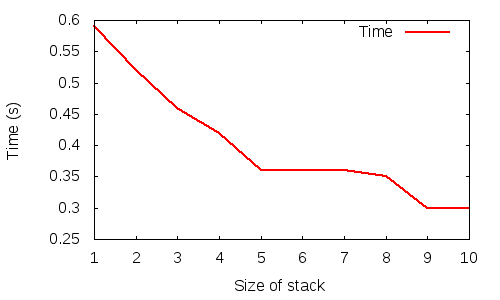
\includegraphics[width=\linewidth]{Shashkova/images/dfs_time.png}}
   \caption{Время работы программы в зависимости от величины стека c алгоритмом Mark (DFS)}
   \label{ris:dtime}   
   \center{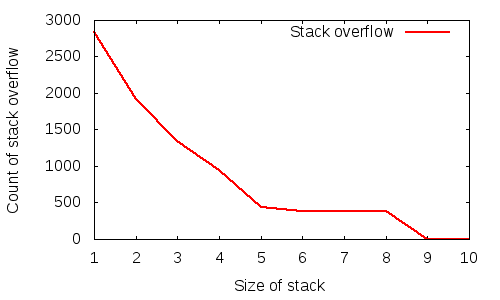
\includegraphics[width=\linewidth]{Shashkova/images/dfs_overflow_count.png}}
   \caption{Количество переполнений стека с алгоритмом Mark (DFS)}  
   \label{ris:dof}
   \end{figure}
   \begin{figure}
   \center{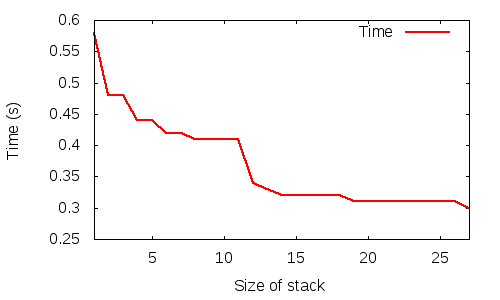
\includegraphics[width=\linewidth]{Shashkova/images/bfs_time.png}}
   \caption{Время работы программы в зависимости от величины стека c алгоритмом Mark (BFS)}
   \label{ris:btime}   
   \center{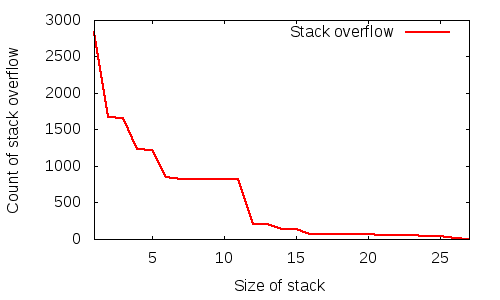
\includegraphics[width=\linewidth]{Shashkova/images/bfs_overflow_count.png}}
   \caption{Количество переполнений стека c алгоритмом Mark (BFS)}
   \label{ris:bof}
   \end{figure}
   

На рис.~\ref{ris:dof} показана зависимость количества переполнений стека от размера стека. Из этого графика хорошо видно, почему график времени работы имеет такую 
неравномерную структуру, а также «ступень». Становится понятно, что время работы программы с переполнениями стека напрямую зависит от количества этих переполнений,
которые происходили в процессе выполнения. И равномерное убывание времени на промежутке от 1 до 5, и постоянное время на промежутке от 5 до 8 полностью объясняется 
зависимостью количества переполнений, которая ведет себя аналогично.

Также были исследованы аналогичные зависимости для алгоритма маркировки с обходом объектов в ширину (Mark (BFS)).

На рис.~\ref{ris:btime} представлена зависимость времени работы программы от величины стека. 
При размере стека, большем 25, переполнения не происходит. Как и в случае с алгоритмом Mark (DFS) в худшем случае (при размере стека $n = 1$) время работы программы
увеличивается почти вдвое. Из особенностей графика можно отметить резкое падение времени работы при увеличении размера стека с 11 до 12. Аналогично для объяснения 
такой зависимости, рассмотрим поведение количества переполнений в зависимости от размера стека.

На рис.~\ref{ris:bof} показана зависимость количества переполнений стека от размера стека с алгоритмом Mark (BFS). Как и в случае с алгоритмом Mark (DFS), очевидно, 
что время работы напрямую зависит от количества происходящих переполнений стека. Резкое падение при изменении размера стека с 11 на 12 также объясняется количеством 
переполнений.

Объясним неравномерность количества переполнений, происходящих при работе каждого из алгоритмов. Будем называть {\it стековой глубиной } корневого объекта максимальную заполненность стека при обходе потомков данного 
корневого объекта.

На графиках рис.~\ref{ris:dm} и рис.~\ref{ris:bm} показано количество корневых объектов в зависимости от их стековой глубины для обоих алгоритмов. 
Из графика рис.~\ref{ris:dm} понятно поведение количества переполнений с алгоритмом Mark (DFS). Количество корневых 
объктов со стековой глубиной от 1 до 5 равномерно убывает, как и убывает количество переполнений. «Ступень» в количестве переполнений также связана с тем, 
что количество корневых объектов стековой глубины больше 5 очень мало по сравнению с объектами меньшей глубины. Поэтому количество переполнений почти не изменяется и 
убывает, только когда переполнения перестают возникать вовсе.

Аналогично для алгоритма Mark (BFS) из рис.~\ref{ris:bm} видно, что количество корневых объектов со стековой глубиной от 8 до 11 и больше 14 мало по сравнению с другими 
объектами, чем и объясняются постоянные промежутки на графике количества переполнений (рис.~\ref{ris:bof}).

   \begin{figure}[p!]   
   \center{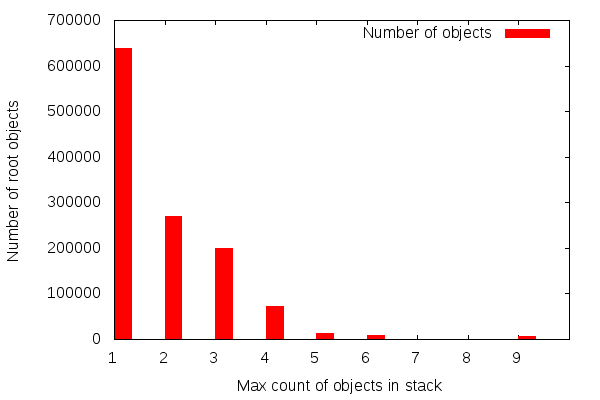
\includegraphics[width=\linewidth]{Shashkova/images/dfs_max_stack.png}}
   \caption{Количество корневых объектов в зависимости от глубины стека с алгоритмом Mark (DFS)}
   \label{ris:dm}   
   \center{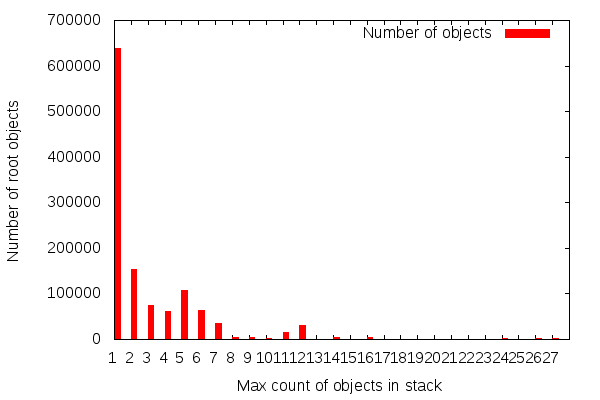
\includegraphics[width=\linewidth]{Shashkova/images/bfs_max_stack.png}}
   \caption{Количество корневых объектов в зависимости от глубины стека с алгоритмом Mark (BFS)}
   \label{ris:bm}   
   \end{figure}


Стоит обратить отдельное внимание на величину стека, при которой происходят переполнения в обоих алгоритмах. Как говорилось ранее, с использованием алгоритма
Mark (BFS) стек перестает переполнятся при размере, большем 9. С алгоритмом Mark (DFS) переполнения происходят вплоть до размера, равного 25. То есть при переходе 
к другому алгоритму размер стека увеличивается почти в 3 раза. Скорее всего, это связано со структурой объектов в тестовой программе. 

Граф, описывающий структуру наших объектов, является лесом из почти деревьев. Под почти деревьями будем понимать традиционные деревья, определенные в теории графов, 
с тем лишь 
отличием, что они могут содержать петли (вершины, связанные ребром сами с собой). Появление петель связано с наличием замыканий (closure) в множестве наших 
объектов. Однако наличие петель не влияет на глубину и ширину дерева, поэтому мы можем считать наши графы деревьями.

Такая значительная разница в размерах стека означает, что у многих деревьев их ширина больше глубины. Анализ объектов в тестовой программе показал, что 
количество потомков у объекта не превышает трех. Даже при небольшой глубине дерева количество объектов на каждом уровне растет довольно быстро, что и приводит 
к увеличению размера используемого стека при обходе в ширину, в отличие от обхода в глубину.

\section*{Заключение}

В результате работы была проведена интеграция бэкенда для языка OCaml и расширения для сборки мусора в LLVM. Было изучено внутреннее 
представление объектов в языке OCaml и реализованы два итеративных алгоритма обхода объектов в стадии пометки сборщика мусора. Результат работы был протестирован
на простейших программах и корректно работает на более сложных примерах. 

\begin{thebibliography}{99}
\bibitem{LLVM} Chris Lattner.
LLVM: An Infrastructure for Multi-Stage Optimization.
Computer Science Dept., University of Illinois at Urbana-Champaign, 2002.

\bibitem{samofal}
Самофалов А.В. Принципы организации сборщика мусора в инфраструктуре LLVM // 
Настоящий сборник.

\bibitem{knuth}
Д. Кнут. Искусство программирования, том 1. Основные алгоритмы.
М.: ``Вильямс»'', 2006.

\bibitem{pliss}
Плисс О.А. Материалы к летней школе ``Управление памятью''. СПбГУ, 2013.

\end{thebibliography}

\title{Сборщик мусора\\
для языка Objective Caml\\
в инфраструктуре LLVM}
%
\titlerunning{Сборщик мусора для языка Objective Caml}
\author{Шашкова Елизавета Михайловна}
%
\authorrunning{Е.М.Шашкова} % abbreviated author list (for running head)
%
%%%% list of authors for the TOC (use if author list has to be modified)
\tocauthor{Е.М.Шашкова}
%
\institute{Санкт-Петербургский государственный университет\\
\email{Elizabeth.Shashkova@gmail.com}}

\maketitle              % typeset the title of the contribution

\section*{Введение}

Сборка мусора --- одна из форм автоматического управления памятью. Специальный компонент поддержки среды времени исполнения, 
называемый сборщиком мусора, автоматически освобождает 
память, удаляя объекты, которые больше не являются доступными для использования.  Сборка мусора освобождает программиста от 
необходимости вручную выделять и освобождать память и позволяет сконцентрироваться на выполнении других задач.
В большинстве современных языков все чаще происходит отказ от предоставления явных средств управления памятью в пользу сборки мусора.

Сборка мусора тесно связана с реализацией компилятора: например, он должен предоставлять сборщику мусора способ определить адреса корневых объектов во
время исполнения. Один из основных
подходов к созданию компиляторов --- использование инфраструктур. Одной из таких инфраструктур построения компиляторов является LLVM 
(Low Level Virtual Machine)~\cite{LLVM}. 

LLVM предназначена 
для анализа, трансформации и оптимизации программ. В основе LLVM лежит промежуточное представление кода 
(Intermediate Representation, IR), над которым можно производить трансформации во время компиляции и компоновки. 
Из этого представления генерируется оптимизированный машинный код для целого ряда платформ.

Objective Caml (OCaml)\footnote{www.caml.inria.fr} --- современный объектно-ориентированный язык функционального программирования общего назначения.
Для языка OCaml существует единственный компилятор от разработчиков самого языка, однако он содержит довольно много платформозависимого кода.
LLVM улучшает переносимость кода между различными платформами и тем самым упрощает процесс построения 
собственного компилятора. Однако язык OCaml требует сборки мусора и реализованный для него бэкенд рассчитывает на наличие сборщика мусора. Но в 
инфраструктуре LLVM нет стандартного способа осуществления сборки мусора, и разработчики предоставили 
возможность для создания расширения LLVM, позволяющего её реализовывать. Данное расширение было реализовано в виде подключаемого модуля~\cite{samofal}.

Целью данной курсовой работы является проведение интеграции бэкенда для языка OCaml и расширения для сборки мусора в LLVM. Необходимо изучить внутреннее 
устройство объектов в языке OCaml и реализвать стадию пометки (mark) для алгоритма сборки мусора mark-and-sweep.

\section{Представление данных в OCaml}

Стадия пометки в алгоритме сборки мусора mark-and-sweep заключается в том, чтобы обойти все "живые" (всё ещё доступные из корневого множества)
объекты и пометить их. Затем на стадии очистки все объекты, которые не были помечены на данной стадии, будут считаться недоступными в программе, а значит,
будут подлежать удалению.

Для реализации стадии пометки необходимо узнать внутреннее устройство объектов.
Все значения в языке OCaml имеют единообразное представление: все они являются типом value языка C (это значение и макросы для работы с ним
определены в файле caml/mlvalues.h). Объект типа value может являться:

\begin{itemize}
   \item целым числом;
   \item указателем на блок внутри кучи;
   \item указателем на блоки вне кучи.
\end{itemize}

Целые числа находятся не в куче, поэтому сборщиком мусора рассматриваться не будут. Блоки, находящиеся в куче, являются основной целью работы сборщика
мусора. Каждый блок содержит заголовок с информацией о длине блока и теге.

Тег определяет структуру блока. Теги со значением меньше, чем \texttt{No\_scan\_tag}, 
означают, что данный блок является корректно структурированным и может быть рекурсивно обойден сборщиком мусора. 
Теги со значением больше, либо равные \texttt{No\_scan\_tag}, означают, что содержимое данного блока должно быть проигнорировано сборщиком мусора. 
Соответствие внутреннего содержимого блоков их тегам показано на рис.~\ref{block_types}.

\begin{figure}[t]
    \begin{tabular}{|l| p{6cm}|}
    \hline
    Тег & Содержимое блока \\
    \hline
    от 0 до \texttt{No\_scan\_tag} -- 1 & Структурированный блок (массив объектов OCaml). Каждое поле является типом value.\\
    \hline
    \texttt{Closure\_tag} & Замыкание представляет собой функциональное значение. Первое слово является указателем на участок кода,
    остальные являются объектами типа value.\\
    \hline
    \texttt{String\_tag} & Строка символов. \\
    \hline
    \texttt{Double\_tag} & Число с плавающей точкой двойной точности. \\
    \hline
    \texttt{Double\_array\_tag} & Массив чисел c плавающей точкой двойной точности. \\
    \hline
    \texttt{Abstract\_tag} & Блок, представляющий абстрактный тип данных. \\
    \hline
    \texttt{Custom\_tag} & Блок, представляющий абстрактный тип данных
    с ``привязанными'' пользовательскими функциями. \\
    \hline
    \end{tabular}
    \caption{Типы блоков в OCaml}
    \label{block_types}
\end{figure}

Благодаря такому устройству объектов становится возможным обход объектов, доступных из живых объектов. Можно быть уверенными,
что в процессе обхода мы не уйдем в область памяти, неинтересную сборщику мусора, а также не пропустим интересующие нас объекты. 

\section{Обход объектов}

Наиболее естественным алгоритмом обхода объектов можно назвать рекурсивный алгоритм. Его описание представлено ниже.
\begin{enumerate}
   \item Алгоритм запускается для каждого корневого объекта.
   \item Проверить, что текущий объект является блоком (а, например, не целым числом).
   \item Если объект является блоком, узнать значение его тега.
   \item Если значение тега меньше значения \texttt{No\_scan\_tag}, объект является живым. Нужно проверить, что
   данный объект находится в куче и пометить его как живой.
   \item Если значение тега больше или равно значению \texttt{No\_scan\_tag}, значит, объект должен игнорироваться сборщиком 
   мусора.
   \item После пометки самого объекта нужно последовательно обойти блоки, содержащиеся внутри данного блока 
   (их количество известно из заголовка) и повторить с ними ту же операцию.
   \item Отдельное внимание нужно уделить объекту с тегом \texttt{Closure\_tag}, так как первое слово является 
   указателем на код и при обходе сборщиком мусора должно игнорироваться.
\end{enumerate}

Однако, рекурсивный вызов функций потребует дополнительной памяти для сохранения стека вызовов, причем размер этого стека предсказать невозможно. Поэтому данный 
алгоритм необходимо было превратить в нерекурсивный, с использованием собственного стека. Структуру объектов программы можно представить в виде графа, где 
вершины --- объекты, а ребра --- ссылки между объектами. Граф можно обойти двумя способами: в ширину (Breadth-first search) и в глубину(Depth-first search).

При обходе в глубину у каждого объекта поочередно просматриваются объекты, на которые он ссылается. Для каждого такого объекта помечаются все его потомки и только 
потом алгоритм переходит к следующему потомку текущего объекта. Код Mark описывает данный алгоритм. Здесь $push()$ и $pop()$ --- операции работы со стеком.

\begin{algorithm}[p]
\caption{Mark}
\label{BFS}
\begin{algorithmic}[1]
    \For {$root \in root\_objects$}
        \If {$is\_object(root)$}
            \If {$tag(root) < No\_scan\_tag$ }
                \If {$root$ in heap}
                    \State {$mark(root)$}
                \EndIf
                \State $push(root)$
                \While {$object \leftarrow pop()$}
                    \State $size \leftarrow size(object)$
                    \If {$tag(object) = Closure\_tag$}
                        \State $i = 1$
                    \Else
                        \State $i = 0$
                    \EndIf
                    \For {$i < size$}
                        \State $child \leftarrow Field(object, i)$
                        \If {   $is\_object(child)$ and\\
                                \hskip\algorithmicindent
                                \hskip\algorithmicindent
                                \hskip\algorithmicindent
                                \hskip\algorithmicindent
                                \hskip\algorithmicindent
                                \hskip\algorithmicindent $tag(child) < No\_scan\_tag$                           
                             }
                            \If {$child$ in heap and not $marked(child)$}
                                \State {$mark(child)$}
                                \State {$push(child)$}
                            \EndIf
                        \EndIf
                    \EndFor
                \EndWhile
            \EndIf
        \EndIf
    \EndFor
    %\EndProcedure
\end{algorithmic}
\end{algorithm}


При обходе в ширину объекты рассматриваются в порядке возрастания расстояния от них до коневого объекта в графе объектов. Данный алгоритм описывается
так же, как и алгоритм Mark, с тем лишь отличием, что вместо стека используется очередь, реализованная на массиве. То есть в данном псевдокоде операции 
$push()$ и $pop()$ --- операции работы с очередью.

Обе модификации данного алгоритма (с обходом в глубину и в ширину) были реализованы итеративно с созданием стека в статической области памяти. 
Отсюда понятно, что размер стека в таком случае является постоянным, и может произойти переполнение стека. Для данной ситуации существует 
специальный алгоритм восстановления.

В случае переполнения стека нельзя допустить некорректную работу сборщика мусора. Если произойдет ошибка в работе стадии пометки, часть живых 
объектов не будут помечены, то есть будут считаться мертвыми и память из-под них будет преждевременно освобождена, что приведет к 
некорректной работе программы. Алгоритм восстановления при переполнении стека был описан в ~\cite{knuth}. Для реализации было решено использовать модификацию 
этого алгоритма~\cite{pliss}. Этот алгоритм, работающий с ограниченной памятью, можно описать следующим образом:

\begin{enumerate}
   \item При заполнении стека алгоритм пометки продолжает свою работу. Однако новые объекты, которые не поместились в стек, в него не добавляются,
   а просто игнорируются.
   \item При переполнении устанавливается специальный флаг, сообщающий о том, что переполнение произошло.
   \item При завершении стадии пометки проверяется состояние флага о переполнении.
   \item Если переполнение произошло, значит, часть живых объектов не была помечена. Начинается последовательный обход кучи.
   \item Флаг переполнения сбрасывается. Начиная с каждого помеченного (то есть точно живого) объекта кучи запускается алгоритм пометки.
   \item Теперь для пометки будет рассматриваться меньше объектов и велика вероятность, что они поместятся в стек. В случае же, если переполнение 
   произойдет снова, алгоритм повторится (снова установится флаг переполнения и т.д.).
\end{enumerate}

Нужно пояснить, что данный алгоритм не будет работать бесконечно долго, так как при каждом последующем запуске стадии пометки мы помечаем 
как минимум $n + 1$ объект из ранее не помеченных (где $n$ --- размер стека). Количество объектов в куче конечно, а значит, процесс когда-нибудь 
закончится. Все живые объекты будут помечены и стадия маркировки корректно выполнит свою задачу даже при условии переполнения стека.

\section{Результаты}
В результате был создан модуль, реализующий стадию маркировки для алгоритма сборки мусора и произведена модификация кучи для обработки переполнения стека.
Реализация была выполнена на языке C. 

Наиболее интересным было исследовать работу программы при переполнении стека. В качестве тестовой программы был взят парсер c С-подобного языка,
написанный на языке OCaml. Он принимает на вход файл для разбора и анализирует его. Во всех экспериментах, представленных ниже, на вход подавался
один и тот же файл. 

Сборка мусора вызывалась автоматически, использовался алгоритм инициализации, основанный на количестве доступной свободной памяти. Согласно 
этому алгоритму, сборка мусора начинается, когда объем занятой памяти в куче превышает некоторый порог, заданный переменной $Threshold$. В данных 
экспериментах значение переменной $Threshold$ равнялось 0.75, что соответствует моментам, когда 75\% объема памяти кучи заняты.  

Благодаря тому, что вызов сборки мусора основывался на количестве доступной памяти, во всех экспериментах количество вызовов сборки мусора было одинаково и равнялось 
1370. К тому же сборка мусора производилась на одинаковых стадиях работы программы.

На рис.~\ref{ris:dtime} представлена зависимость времени работы программы от
величины стека. При размере стека, большем 8, переполнения не происходит. Из графика видно, что переполнение стека значительно, почти в 2 раза, увеличивает 
время работы программы. Из графика видно, что время работы равномерно убывает при изменении размера стека от 1 до 5. При дальнейшем увеличении размера стека, 
на графике заметна некоторая «ступень»: при увеличении размера стека от 5 до 8 время работы программы почти не изменяется. И лишь после этого оно еще раз уменьшается 
и перестает зависеть от дальнейшего увеличения стека. 

Для исследования такого поведения, исследуем количество переполнений, происходящих при работе программы.

   \begin{figure}[p]   
   \center{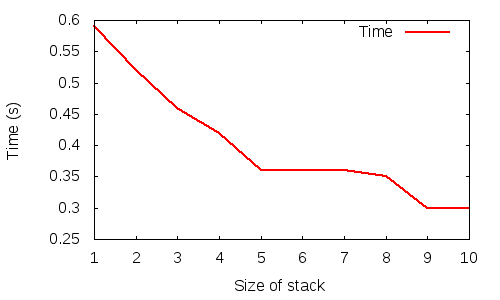
\includegraphics[width=\linewidth]{Shashkova/images/dfs_time.png}}
   \caption{Время работы программы в зависимости от величины стека c алгоритмом Mark (DFS)}
   \label{ris:dtime}   
   \center{\includegraphics[width=\linewidth]{Shashkova/images/dfs_overflow_count.png}}
   \caption{Количество переполнений стека с алгоритмом Mark (DFS)}  
   \label{ris:dof}
   \end{figure}
   \begin{figure}
   \center{\includegraphics[width=\linewidth]{Shashkova/images/bfs_time.png}}
   \caption{Время работы программы в зависимости от величины стека c алгоритмом Mark (BFS)}
   \label{ris:btime}   
   \center{\includegraphics[width=\linewidth]{Shashkova/images/bfs_overflow_count.png}}
   \caption{Количество переполнений стека c алгоритмом Mark (BFS)}
   \label{ris:bof}
   \end{figure}
   

На рис.~\ref{ris:dof} показана зависимость количества переполнений стека от размера стека. Из этого графика хорошо видно, почему график времени работы имеет такую 
неравномерную структуру, а также «ступень». Становится понятно, что время работы программы с переполнениями стека напрямую зависит от количества этих переполнений,
которые происходили в процессе выполнения. И равномерное убывание времени на промежутке от 1 до 5, и постоянное время на промежутке от 5 до 8 полностью объясняется 
зависимостью количества переполнений, которая ведет себя аналогично.

Также были исследованы аналогичные зависимости для алгоритма маркировки с обходом объектов в ширину (Mark (BFS)).

На рис.~\ref{ris:btime} представлена зависимость времени работы программы от величины стека. 
При размере стека, большем 25, переполнения не происходит. Как и в случае с алгоритмом Mark (DFS) в худшем случае (при размере стека $n = 1$) время работы программы
увеличивается почти вдвое. Из особенностей графика можно отметить резкое падение времени работы при увеличении размера стека с 11 до 12. Аналогично для объяснения 
такой зависимости, рассмотрим поведение количества переполнений в зависимости от размера стека.

На рис.~\ref{ris:bof} показана зависимость количества переполнений стека от размера стека с алгоритмом Mark (BFS). Как и в случае с алгоритмом Mark (DFS), очевидно, 
что время работы напрямую зависит от количества происходящих переполнений стека. Резкое падение при изменении размера стека с 11 на 12 также объясняется количеством 
переполнений.

Объясним неравномерность количества переполнений, происходящих при работе каждого из алгоритмов. Будем называть {\it стековой глубиной } корневого объекта максимальную заполненность стека при обходе потомков данного 
корневого объекта.

На графиках рис.~\ref{ris:dm} и рис.~\ref{ris:bm} показано количество корневых объектов в зависимости от их стековой глубины для обоих алгоритмов. 
Из графика рис.~\ref{ris:dm} понятно поведение количества переполнений с алгоритмом Mark (DFS). Количество корневых 
объктов со стековой глубиной от 1 до 5 равномерно убывает, как и убывает количество переполнений. «Ступень» в количестве переполнений также связана с тем, 
что количество корневых объектов стековой глубины больше 5 очень мало по сравнению с объектами меньшей глубины. Поэтому количество переполнений почти не изменяется и 
убывает, только когда переполнения перестают возникать вовсе.

Аналогично для алгоритма Mark (BFS) из рис.~\ref{ris:bm} видно, что количество корневых объектов со стековой глубиной от 8 до 11 и больше 14 мало по сравнению с другими 
объектами, чем и объясняются постоянные промежутки на графике количества переполнений (рис.~\ref{ris:bof}).

   \begin{figure}[p!]   
   \center{\includegraphics[width=\linewidth]{Shashkova/images/dfs_max_stack.png}}
   \caption{Количество корневых объектов в зависимости от глубины стека с алгоритмом Mark (DFS)}
   \label{ris:dm}   
   \center{\includegraphics[width=\linewidth]{Shashkova/images/bfs_max_stack.png}}
   \caption{Количество корневых объектов в зависимости от глубины стека с алгоритмом Mark (BFS)}
   \label{ris:bm}   
   \end{figure}


Стоит обратить отдельное внимание на величину стека, при которой происходят переполнения в обоих алгоритмах. Как говорилось ранее, с использованием алгоритма
Mark (BFS) стек перестает переполнятся при размере, большем 9. С алгоритмом Mark (DFS) переполнения происходят вплоть до размера, равного 25. То есть при переходе 
к другому алгоритму размер стека увеличивается почти в 3 раза. Скорее всего, это связано со структурой объектов в тестовой программе. 

Граф, описывающий структуру наших объектов, является лесом из почти деревьев. Под почти деревьями будем понимать традиционные деревья, определенные в теории графов, 
с тем лишь 
отличием, что они могут содержать петли (вершины, связанные ребром сами с собой). Появление петель связано с наличием замыканий (closure) в множестве наших 
объектов. Однако наличие петель не влияет на глубину и ширину дерева, поэтому мы можем считать наши графы деревьями.

Такая значительная разница в размерах стека означает, что у многих деревьев их ширина больше глубины. Анализ объектов в тестовой программе показал, что 
количество потомков у объекта не превышает трех. Даже при небольшой глубине дерева количество объектов на каждом уровне растет довольно быстро, что и приводит 
к увеличению размера используемого стека при обходе в ширину, в отличие от обхода в глубину.

\section*{Заключение}

В результате работы была проведена интеграция бэкенда для языка OCaml и расширения для сборки мусора в LLVM. Было изучено внутреннее 
представление объектов в языке OCaml и реализованы два итеративных алгоритма обхода объектов в стадии пометки сборщика мусора. Результат работы был протестирован
на простейших программах и корректно работает на более сложных примерах. 

\begin{thebibliography}{99}
\bibitem{LLVM} Chris Lattner.
LLVM: An Infrastructure for Multi-Stage Optimization.
Computer Science Dept., University of Illinois at Urbana-Champaign, 2002.

\bibitem{samofal}
Самофалов А.В. Принципы организации сборщика мусора в инфраструктуре LLVM // 
Настоящий сборник.

\bibitem{knuth}
Д. Кнут. Искусство программирования, том 1. Основные алгоритмы.
М.: ``Вильямс»'', 2006.

\bibitem{pliss}
Плисс О.А. Материалы к летней школе ``Управление памятью''. СПбГУ, 2013.

\end{thebibliography}


\title{Сборщик мусора\\
для языка Objective Caml\\
в инфраструктуре LLVM}
%
\titlerunning{Сборщик мусора для языка Objective Caml}
\author{Шашкова Елизавета Михайловна}
%
\authorrunning{Е.М.Шашкова} % abbreviated author list (for running head)
%
%%%% list of authors for the TOC (use if author list has to be modified)
\tocauthor{Е.М.Шашкова}
%
\institute{Санкт-Петербургский государственный университет\\
\email{Elizabeth.Shashkova@gmail.com}}

\maketitle              % typeset the title of the contribution

\section*{Введение}

Сборка мусора --- одна из форм автоматического управления памятью. Специальный компонент поддержки среды времени исполнения, 
называемый сборщиком мусора, автоматически освобождает 
память, удаляя объекты, которые больше не являются доступными для использования.  Сборка мусора освобождает программиста от 
необходимости вручную выделять и освобождать память и позволяет сконцентрироваться на выполнении других задач.
В большинстве современных языков все чаще происходит отказ от предоставления явных средств управления памятью в пользу сборки мусора.

Сборка мусора тесно связана с реализацией компилятора: например, он должен предоставлять сборщику мусора способ определить адреса корневых объектов во
время исполнения. Один из основных
подходов к созданию компиляторов --- использование инфраструктур. Одной из таких инфраструктур построения компиляторов является LLVM 
(Low Level Virtual Machine)~\cite{LLVM}. 

LLVM предназначена 
для анализа, трансформации и оптимизации программ. В основе LLVM лежит промежуточное представление кода 
(Intermediate Representation, IR), над которым можно производить трансформации во время компиляции и компоновки. 
Из этого представления генерируется оптимизированный машинный код для целого ряда платформ.

Objective Caml (OCaml)\footnote{www.caml.inria.fr} --- современный объектно-ориентированный язык функционального программирования общего назначения.
Для языка OCaml существует единственный компилятор от разработчиков самого языка, однако он содержит довольно много платформозависимого кода.
LLVM улучшает переносимость кода между различными платформами и тем самым упрощает процесс построения 
собственного компилятора. Однако язык OCaml требует сборки мусора и реализованный для него бэкенд рассчитывает на наличие сборщика мусора. Но в 
инфраструктуре LLVM нет стандартного способа осуществления сборки мусора, и разработчики предоставили 
возможность для создания расширения LLVM, позволяющего её реализовывать. Данное расширение было реализовано в виде подключаемого модуля~\cite{samofal}.

Целью данной курсовой работы является проведение интеграции бэкенда для языка OCaml и расширения для сборки мусора в LLVM. Необходимо изучить внутреннее 
устройство объектов в языке OCaml и реализвать стадию пометки (mark) для алгоритма сборки мусора mark-and-sweep.

\section{Представление данных в OCaml}

Стадия пометки в алгоритме сборки мусора mark-and-sweep заключается в том, чтобы обойти все "живые" (всё ещё доступные из корневого множества)
объекты и пометить их. Затем на стадии очистки все объекты, которые не были помечены на данной стадии, будут считаться недоступными в программе, а значит,
будут подлежать удалению.

Для реализации стадии пометки необходимо узнать внутреннее устройство объектов.
Все значения в языке OCaml имеют единообразное представление: все они являются типом value языка C (это значение и макросы для работы с ним
определены в файле caml/mlvalues.h). Объект типа value может являться:

\begin{itemize}
   \item целым числом;
   \item указателем на блок внутри кучи;
   \item указателем на блоки вне кучи.
\end{itemize}

Целые числа находятся не в куче, поэтому сборщиком мусора рассматриваться не будут. Блоки, находящиеся в куче, являются основной целью работы сборщика
мусора. Каждый блок содержит заголовок с информацией о длине блока и теге.

Тег определяет структуру блока. Теги со значением меньше, чем \texttt{No\_scan\_tag}, 
означают, что данный блок является корректно структурированным и может быть рекурсивно обойден сборщиком мусора. 
Теги со значением больше, либо равные \texttt{No\_scan\_tag}, означают, что содержимое данного блока должно быть проигнорировано сборщиком мусора. 
Соответствие внутреннего содержимого блоков их тегам показано на рис.~\ref{block_types}.

\begin{figure}[t]
    \begin{tabular}{|l| p{6cm}|}
    \hline
    Тег & Содержимое блока \\
    \hline
    от 0 до \texttt{No\_scan\_tag} -- 1 & Структурированный блок (массив объектов OCaml). Каждое поле является типом value.\\
    \hline
    \texttt{Closure\_tag} & Замыкание представляет собой функциональное значение. Первое слово является указателем на участок кода,
    остальные являются объектами типа value.\\
    \hline
    \texttt{String\_tag} & Строка символов. \\
    \hline
    \texttt{Double\_tag} & Число с плавающей точкой двойной точности. \\
    \hline
    \texttt{Double\_array\_tag} & Массив чисел c плавающей точкой двойной точности. \\
    \hline
    \texttt{Abstract\_tag} & Блок, представляющий абстрактный тип данных. \\
    \hline
    \texttt{Custom\_tag} & Блок, представляющий абстрактный тип данных
    с ``привязанными'' пользовательскими функциями. \\
    \hline
    \end{tabular}
    \caption{Типы блоков в OCaml}
    \label{block_types}
\end{figure}

Благодаря такому устройству объектов становится возможным обход объектов, доступных из живых объектов. Можно быть уверенными,
что в процессе обхода мы не уйдем в область памяти, неинтересную сборщику мусора, а также не пропустим интересующие нас объекты. 

\section{Обход объектов}

Наиболее естественным алгоритмом обхода объектов можно назвать рекурсивный алгоритм. Его описание представлено ниже.
\begin{enumerate}
   \item Алгоритм запускается для каждого корневого объекта.
   \item Проверить, что текущий объект является блоком (а, например, не целым числом).
   \item Если объект является блоком, узнать значение его тега.
   \item Если значение тега меньше значения \texttt{No\_scan\_tag}, объект является живым. Нужно проверить, что
   данный объект находится в куче и пометить его как живой.
   \item Если значение тега больше или равно значению \texttt{No\_scan\_tag}, значит, объект должен игнорироваться сборщиком 
   мусора.
   \item После пометки самого объекта нужно последовательно обойти блоки, содержащиеся внутри данного блока 
   (их количество известно из заголовка) и повторить с ними ту же операцию.
   \item Отдельное внимание нужно уделить объекту с тегом \texttt{Closure\_tag}, так как первое слово является 
   указателем на код и при обходе сборщиком мусора должно игнорироваться.
\end{enumerate}

Однако, рекурсивный вызов функций потребует дополнительной памяти для сохранения стека вызовов, причем размер этого стека предсказать невозможно. Поэтому данный 
алгоритм необходимо было превратить в нерекурсивный, с использованием собственного стека. Структуру объектов программы можно представить в виде графа, где 
вершины --- объекты, а ребра --- ссылки между объектами. Граф можно обойти двумя способами: в ширину (Breadth-first search) и в глубину(Depth-first search).

При обходе в глубину у каждого объекта поочередно просматриваются объекты, на которые он ссылается. Для каждого такого объекта помечаются все его потомки и только 
потом алгоритм переходит к следующему потомку текущего объекта. Код Mark описывает данный алгоритм. Здесь $push()$ и $pop()$ --- операции работы со стеком.

\begin{algorithm}[p]
\caption{Mark}
\label{BFS}
\begin{algorithmic}[1]
    \For {$root \in root\_objects$}
        \If {$is\_object(root)$}
            \If {$tag(root) < No\_scan\_tag$ }
                \If {$root$ in heap}
                    \State {$mark(root)$}
                \EndIf
                \State $push(root)$
                \While {$object \leftarrow pop()$}
                    \State $size \leftarrow size(object)$
                    \If {$tag(object) = Closure\_tag$}
                        \State $i = 1$
                    \Else
                        \State $i = 0$
                    \EndIf
                    \For {$i < size$}
                        \State $child \leftarrow Field(object, i)$
                        \If {   $is\_object(child)$ and\\
                                \hskip\algorithmicindent
                                \hskip\algorithmicindent
                                \hskip\algorithmicindent
                                \hskip\algorithmicindent
                                \hskip\algorithmicindent
                                \hskip\algorithmicindent $tag(child) < No\_scan\_tag$                           
                             }
                            \If {$child$ in heap and not $marked(child)$}
                                \State {$mark(child)$}
                                \State {$push(child)$}
                            \EndIf
                        \EndIf
                    \EndFor
                \EndWhile
            \EndIf
        \EndIf
    \EndFor
    %\EndProcedure
\end{algorithmic}
\end{algorithm}


При обходе в ширину объекты рассматриваются в порядке возрастания расстояния от них до коневого объекта в графе объектов. Данный алгоритм описывается
так же, как и алгоритм Mark, с тем лишь отличием, что вместо стека используется очередь, реализованная на массиве. То есть в данном псевдокоде операции 
$push()$ и $pop()$ --- операции работы с очередью.

Обе модификации данного алгоритма (с обходом в глубину и в ширину) были реализованы итеративно с созданием стека в статической области памяти. 
Отсюда понятно, что размер стека в таком случае является постоянным, и может произойти переполнение стека. Для данной ситуации существует 
специальный алгоритм восстановления.

В случае переполнения стека нельзя допустить некорректную работу сборщика мусора. Если произойдет ошибка в работе стадии пометки, часть живых 
объектов не будут помечены, то есть будут считаться мертвыми и память из-под них будет преждевременно освобождена, что приведет к 
некорректной работе программы. Алгоритм восстановления при переполнении стека был описан в ~\cite{knuth}. Для реализации было решено использовать модификацию 
этого алгоритма~\cite{pliss}. Этот алгоритм, работающий с ограниченной памятью, можно описать следующим образом:

\begin{enumerate}
   \item При заполнении стека алгоритм пометки продолжает свою работу. Однако новые объекты, которые не поместились в стек, в него не добавляются,
   а просто игнорируются.
   \item При переполнении устанавливается специальный флаг, сообщающий о том, что переполнение произошло.
   \item При завершении стадии пометки проверяется состояние флага о переполнении.
   \item Если переполнение произошло, значит, часть живых объектов не была помечена. Начинается последовательный обход кучи.
   \item Флаг переполнения сбрасывается. Начиная с каждого помеченного (то есть точно живого) объекта кучи запускается алгоритм пометки.
   \item Теперь для пометки будет рассматриваться меньше объектов и велика вероятность, что они поместятся в стек. В случае же, если переполнение 
   произойдет снова, алгоритм повторится (снова установится флаг переполнения и т.д.).
\end{enumerate}

Нужно пояснить, что данный алгоритм не будет работать бесконечно долго, так как при каждом последующем запуске стадии пометки мы помечаем 
как минимум $n + 1$ объект из ранее не помеченных (где $n$ --- размер стека). Количество объектов в куче конечно, а значит, процесс когда-нибудь 
закончится. Все живые объекты будут помечены и стадия маркировки корректно выполнит свою задачу даже при условии переполнения стека.

\section{Результаты}
В результате был создан модуль, реализующий стадию маркировки для алгоритма сборки мусора и произведена модификация кучи для обработки переполнения стека.
Реализация была выполнена на языке C. 

Наиболее интересным было исследовать работу программы при переполнении стека. В качестве тестовой программы был взят парсер c С-подобного языка,
написанный на языке OCaml. Он принимает на вход файл для разбора и анализирует его. Во всех экспериментах, представленных ниже, на вход подавался
один и тот же файл. 

Сборка мусора вызывалась автоматически, использовался алгоритм инициализации, основанный на количестве доступной свободной памяти. Согласно 
этому алгоритму, сборка мусора начинается, когда объем занятой памяти в куче превышает некоторый порог, заданный переменной $Threshold$. В данных 
экспериментах значение переменной $Threshold$ равнялось 0.75, что соответствует моментам, когда 75\% объема памяти кучи заняты.  

Благодаря тому, что вызов сборки мусора основывался на количестве доступной памяти, во всех экспериментах количество вызовов сборки мусора было одинаково и равнялось 
1370. К тому же сборка мусора производилась на одинаковых стадиях работы программы.

На рис.~\ref{ris:dtime} представлена зависимость времени работы программы от
величины стека. При размере стека, большем 8, переполнения не происходит. Из графика видно, что переполнение стека значительно, почти в 2 раза, увеличивает 
время работы программы. Из графика видно, что время работы равномерно убывает при изменении размера стека от 1 до 5. При дальнейшем увеличении размера стека, 
на графике заметна некоторая «ступень»: при увеличении размера стека от 5 до 8 время работы программы почти не изменяется. И лишь после этого оно еще раз уменьшается 
и перестает зависеть от дальнейшего увеличения стека. 

Для исследования такого поведения, исследуем количество переполнений, происходящих при работе программы.

   \begin{figure}[p]   
   \center{\includegraphics[width=\linewidth]{Shashkova/images/dfs_time.png}}
   \caption{Время работы программы в зависимости от величины стека c алгоритмом Mark (DFS)}
   \label{ris:dtime}   
   \center{\includegraphics[width=\linewidth]{Shashkova/images/dfs_overflow_count.png}}
   \caption{Количество переполнений стека с алгоритмом Mark (DFS)}  
   \label{ris:dof}
   \end{figure}
   \begin{figure}
   \center{\includegraphics[width=\linewidth]{Shashkova/images/bfs_time.png}}
   \caption{Время работы программы в зависимости от величины стека c алгоритмом Mark (BFS)}
   \label{ris:btime}   
   \center{\includegraphics[width=\linewidth]{Shashkova/images/bfs_overflow_count.png}}
   \caption{Количество переполнений стека c алгоритмом Mark (BFS)}
   \label{ris:bof}
   \end{figure}
   

На рис.~\ref{ris:dof} показана зависимость количества переполнений стека от размера стека. Из этого графика хорошо видно, почему график времени работы имеет такую 
неравномерную структуру, а также «ступень». Становится понятно, что время работы программы с переполнениями стека напрямую зависит от количества этих переполнений,
которые происходили в процессе выполнения. И равномерное убывание времени на промежутке от 1 до 5, и постоянное время на промежутке от 5 до 8 полностью объясняется 
зависимостью количества переполнений, которая ведет себя аналогично.

Также были исследованы аналогичные зависимости для алгоритма маркировки с обходом объектов в ширину (Mark (BFS)).

На рис.~\ref{ris:btime} представлена зависимость времени работы программы от величины стека. 
При размере стека, большем 25, переполнения не происходит. Как и в случае с алгоритмом Mark (DFS) в худшем случае (при размере стека $n = 1$) время работы программы
увеличивается почти вдвое. Из особенностей графика можно отметить резкое падение времени работы при увеличении размера стека с 11 до 12. Аналогично для объяснения 
такой зависимости, рассмотрим поведение количества переполнений в зависимости от размера стека.

На рис.~\ref{ris:bof} показана зависимость количества переполнений стека от размера стека с алгоритмом Mark (BFS). Как и в случае с алгоритмом Mark (DFS), очевидно, 
что время работы напрямую зависит от количества происходящих переполнений стека. Резкое падение при изменении размера стека с 11 на 12 также объясняется количеством 
переполнений.

Объясним неравномерность количества переполнений, происходящих при работе каждого из алгоритмов. Будем называть {\it стековой глубиной } корневого объекта максимальную заполненность стека при обходе потомков данного 
корневого объекта.

На графиках рис.~\ref{ris:dm} и рис.~\ref{ris:bm} показано количество корневых объектов в зависимости от их стековой глубины для обоих алгоритмов. 
Из графика рис.~\ref{ris:dm} понятно поведение количества переполнений с алгоритмом Mark (DFS). Количество корневых 
объктов со стековой глубиной от 1 до 5 равномерно убывает, как и убывает количество переполнений. «Ступень» в количестве переполнений также связана с тем, 
что количество корневых объектов стековой глубины больше 5 очень мало по сравнению с объектами меньшей глубины. Поэтому количество переполнений почти не изменяется и 
убывает, только когда переполнения перестают возникать вовсе.

Аналогично для алгоритма Mark (BFS) из рис.~\ref{ris:bm} видно, что количество корневых объектов со стековой глубиной от 8 до 11 и больше 14 мало по сравнению с другими 
объектами, чем и объясняются постоянные промежутки на графике количества переполнений (рис.~\ref{ris:bof}).

   \begin{figure}[p!]   
   \center{\includegraphics[width=\linewidth]{Shashkova/images/dfs_max_stack.png}}
   \caption{Количество корневых объектов в зависимости от глубины стека с алгоритмом Mark (DFS)}
   \label{ris:dm}   
   \center{\includegraphics[width=\linewidth]{Shashkova/images/bfs_max_stack.png}}
   \caption{Количество корневых объектов в зависимости от глубины стека с алгоритмом Mark (BFS)}
   \label{ris:bm}   
   \end{figure}


Стоит обратить отдельное внимание на величину стека, при которой происходят переполнения в обоих алгоритмах. Как говорилось ранее, с использованием алгоритма
Mark (BFS) стек перестает переполнятся при размере, большем 9. С алгоритмом Mark (DFS) переполнения происходят вплоть до размера, равного 25. То есть при переходе 
к другому алгоритму размер стека увеличивается почти в 3 раза. Скорее всего, это связано со структурой объектов в тестовой программе. 

Граф, описывающий структуру наших объектов, является лесом из почти деревьев. Под почти деревьями будем понимать традиционные деревья, определенные в теории графов, 
с тем лишь 
отличием, что они могут содержать петли (вершины, связанные ребром сами с собой). Появление петель связано с наличием замыканий (closure) в множестве наших 
объектов. Однако наличие петель не влияет на глубину и ширину дерева, поэтому мы можем считать наши графы деревьями.

Такая значительная разница в размерах стека означает, что у многих деревьев их ширина больше глубины. Анализ объектов в тестовой программе показал, что 
количество потомков у объекта не превышает трех. Даже при небольшой глубине дерева количество объектов на каждом уровне растет довольно быстро, что и приводит 
к увеличению размера используемого стека при обходе в ширину, в отличие от обхода в глубину.

\section*{Заключение}

В результате работы была проведена интеграция бэкенда для языка OCaml и расширения для сборки мусора в LLVM. Было изучено внутреннее 
представление объектов в языке OCaml и реализованы два итеративных алгоритма обхода объектов в стадии пометки сборщика мусора. Результат работы был протестирован
на простейших программах и корректно работает на более сложных примерах. 

\begin{thebibliography}{99}
\bibitem{LLVM} Chris Lattner.
LLVM: An Infrastructure for Multi-Stage Optimization.
Computer Science Dept., University of Illinois at Urbana-Champaign, 2002.

\bibitem{samofal}
Самофалов А.В. Принципы организации сборщика мусора в инфраструктуре LLVM // 
Настоящий сборник.

\bibitem{knuth}
Д. Кнут. Искусство программирования, том 1. Основные алгоритмы.
М.: ``Вильямс»'', 2006.

\bibitem{pliss}
Плисс О.А. Материалы к летней школе ``Управление памятью''. СПбГУ, 2013.

\end{thebibliography}

\title{Сборщик мусора\\
для языка Objective Caml\\
в инфраструктуре LLVM}
%
\titlerunning{Сборщик мусора для языка Objective Caml}
\author{Шашкова Елизавета Михайловна}
%
\authorrunning{Е.М.Шашкова} % abbreviated author list (for running head)
%
%%%% list of authors for the TOC (use if author list has to be modified)
\tocauthor{Е.М.Шашкова}
%
\institute{Санкт-Петербургский государственный университет\\
\email{Elizabeth.Shashkova@gmail.com}}

\maketitle              % typeset the title of the contribution

\section*{Введение}

Сборка мусора --- одна из форм автоматического управления памятью. Специальный компонент поддержки среды времени исполнения, 
называемый сборщиком мусора, автоматически освобождает 
память, удаляя объекты, которые больше не являются доступными для использования.  Сборка мусора освобождает программиста от 
необходимости вручную выделять и освобождать память и позволяет сконцентрироваться на выполнении других задач.
В большинстве современных языков все чаще происходит отказ от предоставления явных средств управления памятью в пользу сборки мусора.

Сборка мусора тесно связана с реализацией компилятора: например, он должен предоставлять сборщику мусора способ определить адреса корневых объектов во
время исполнения. Один из основных
подходов к созданию компиляторов --- использование инфраструктур. Одной из таких инфраструктур построения компиляторов является LLVM 
(Low Level Virtual Machine)~\cite{LLVM}. 

LLVM предназначена 
для анализа, трансформации и оптимизации программ. В основе LLVM лежит промежуточное представление кода 
(Intermediate Representation, IR), над которым можно производить трансформации во время компиляции и компоновки. 
Из этого представления генерируется оптимизированный машинный код для целого ряда платформ.

Objective Caml (OCaml)\footnote{www.caml.inria.fr} --- современный объектно-ориентированный язык функционального программирования общего назначения.
Для языка OCaml существует единственный компилятор от разработчиков самого языка, однако он содержит довольно много платформозависимого кода.
LLVM улучшает переносимость кода между различными платформами и тем самым упрощает процесс построения 
собственного компилятора. Однако язык OCaml требует сборки мусора и реализованный для него бэкенд рассчитывает на наличие сборщика мусора. Но в 
инфраструктуре LLVM нет стандартного способа осуществления сборки мусора, и разработчики предоставили 
возможность для создания расширения LLVM, позволяющего её реализовывать. Данное расширение было реализовано в виде подключаемого модуля~\cite{samofal}.

Целью данной курсовой работы является проведение интеграции бэкенда для языка OCaml и расширения для сборки мусора в LLVM. Необходимо изучить внутреннее 
устройство объектов в языке OCaml и реализвать стадию пометки (mark) для алгоритма сборки мусора mark-and-sweep.

\section{Представление данных в OCaml}

Стадия пометки в алгоритме сборки мусора mark-and-sweep заключается в том, чтобы обойти все "живые" (всё ещё доступные из корневого множества)
объекты и пометить их. Затем на стадии очистки все объекты, которые не были помечены на данной стадии, будут считаться недоступными в программе, а значит,
будут подлежать удалению.

Для реализации стадии пометки необходимо узнать внутреннее устройство объектов.
Все значения в языке OCaml имеют единообразное представление: все они являются типом value языка C (это значение и макросы для работы с ним
определены в файле caml/mlvalues.h). Объект типа value может являться:

\begin{itemize}
   \item целым числом;
   \item указателем на блок внутри кучи;
   \item указателем на блоки вне кучи.
\end{itemize}

Целые числа находятся не в куче, поэтому сборщиком мусора рассматриваться не будут. Блоки, находящиеся в куче, являются основной целью работы сборщика
мусора. Каждый блок содержит заголовок с информацией о длине блока и теге.

Тег определяет структуру блока. Теги со значением меньше, чем \texttt{No\_scan\_tag}, 
означают, что данный блок является корректно структурированным и может быть рекурсивно обойден сборщиком мусора. 
Теги со значением больше, либо равные \texttt{No\_scan\_tag}, означают, что содержимое данного блока должно быть проигнорировано сборщиком мусора. 
Соответствие внутреннего содержимого блоков их тегам показано на рис.~\ref{block_types}.

\begin{figure}[t]
    \begin{tabular}{|l| p{6cm}|}
    \hline
    Тег & Содержимое блока \\
    \hline
    от 0 до \texttt{No\_scan\_tag} -- 1 & Структурированный блок (массив объектов OCaml). Каждое поле является типом value.\\
    \hline
    \texttt{Closure\_tag} & Замыкание представляет собой функциональное значение. Первое слово является указателем на участок кода,
    остальные являются объектами типа value.\\
    \hline
    \texttt{String\_tag} & Строка символов. \\
    \hline
    \texttt{Double\_tag} & Число с плавающей точкой двойной точности. \\
    \hline
    \texttt{Double\_array\_tag} & Массив чисел c плавающей точкой двойной точности. \\
    \hline
    \texttt{Abstract\_tag} & Блок, представляющий абстрактный тип данных. \\
    \hline
    \texttt{Custom\_tag} & Блок, представляющий абстрактный тип данных
    с ``привязанными'' пользовательскими функциями. \\
    \hline
    \end{tabular}
    \caption{Типы блоков в OCaml}
    \label{block_types}
\end{figure}

Благодаря такому устройству объектов становится возможным обход объектов, доступных из живых объектов. Можно быть уверенными,
что в процессе обхода мы не уйдем в область памяти, неинтересную сборщику мусора, а также не пропустим интересующие нас объекты. 

\section{Обход объектов}

Наиболее естественным алгоритмом обхода объектов можно назвать рекурсивный алгоритм. Его описание представлено ниже.
\begin{enumerate}
   \item Алгоритм запускается для каждого корневого объекта.
   \item Проверить, что текущий объект является блоком (а, например, не целым числом).
   \item Если объект является блоком, узнать значение его тега.
   \item Если значение тега меньше значения \texttt{No\_scan\_tag}, объект является живым. Нужно проверить, что
   данный объект находится в куче и пометить его как живой.
   \item Если значение тега больше или равно значению \texttt{No\_scan\_tag}, значит, объект должен игнорироваться сборщиком 
   мусора.
   \item После пометки самого объекта нужно последовательно обойти блоки, содержащиеся внутри данного блока 
   (их количество известно из заголовка) и повторить с ними ту же операцию.
   \item Отдельное внимание нужно уделить объекту с тегом \texttt{Closure\_tag}, так как первое слово является 
   указателем на код и при обходе сборщиком мусора должно игнорироваться.
\end{enumerate}

Однако, рекурсивный вызов функций потребует дополнительной памяти для сохранения стека вызовов, причем размер этого стека предсказать невозможно. Поэтому данный 
алгоритм необходимо было превратить в нерекурсивный, с использованием собственного стека. Структуру объектов программы можно представить в виде графа, где 
вершины --- объекты, а ребра --- ссылки между объектами. Граф можно обойти двумя способами: в ширину (Breadth-first search) и в глубину(Depth-first search).

При обходе в глубину у каждого объекта поочередно просматриваются объекты, на которые он ссылается. Для каждого такого объекта помечаются все его потомки и только 
потом алгоритм переходит к следующему потомку текущего объекта. Код Mark описывает данный алгоритм. Здесь $push()$ и $pop()$ --- операции работы со стеком.

\begin{algorithm}[p]
\caption{Mark}
\label{BFS}
\begin{algorithmic}[1]
    \For {$root \in root\_objects$}
        \If {$is\_object(root)$}
            \If {$tag(root) < No\_scan\_tag$ }
                \If {$root$ in heap}
                    \State {$mark(root)$}
                \EndIf
                \State $push(root)$
                \While {$object \leftarrow pop()$}
                    \State $size \leftarrow size(object)$
                    \If {$tag(object) = Closure\_tag$}
                        \State $i = 1$
                    \Else
                        \State $i = 0$
                    \EndIf
                    \For {$i < size$}
                        \State $child \leftarrow Field(object, i)$
                        \If {   $is\_object(child)$ and\\
                                \hskip\algorithmicindent
                                \hskip\algorithmicindent
                                \hskip\algorithmicindent
                                \hskip\algorithmicindent
                                \hskip\algorithmicindent
                                \hskip\algorithmicindent $tag(child) < No\_scan\_tag$                           
                             }
                            \If {$child$ in heap and not $marked(child)$}
                                \State {$mark(child)$}
                                \State {$push(child)$}
                            \EndIf
                        \EndIf
                    \EndFor
                \EndWhile
            \EndIf
        \EndIf
    \EndFor
    %\EndProcedure
\end{algorithmic}
\end{algorithm}


При обходе в ширину объекты рассматриваются в порядке возрастания расстояния от них до коневого объекта в графе объектов. Данный алгоритм описывается
так же, как и алгоритм Mark, с тем лишь отличием, что вместо стека используется очередь, реализованная на массиве. То есть в данном псевдокоде операции 
$push()$ и $pop()$ --- операции работы с очередью.

Обе модификации данного алгоритма (с обходом в глубину и в ширину) были реализованы итеративно с созданием стека в статической области памяти. 
Отсюда понятно, что размер стека в таком случае является постоянным, и может произойти переполнение стека. Для данной ситуации существует 
специальный алгоритм восстановления.

В случае переполнения стека нельзя допустить некорректную работу сборщика мусора. Если произойдет ошибка в работе стадии пометки, часть живых 
объектов не будут помечены, то есть будут считаться мертвыми и память из-под них будет преждевременно освобождена, что приведет к 
некорректной работе программы. Алгоритм восстановления при переполнении стека был описан в ~\cite{knuth}. Для реализации было решено использовать модификацию 
этого алгоритма~\cite{pliss}. Этот алгоритм, работающий с ограниченной памятью, можно описать следующим образом:

\begin{enumerate}
   \item При заполнении стека алгоритм пометки продолжает свою работу. Однако новые объекты, которые не поместились в стек, в него не добавляются,
   а просто игнорируются.
   \item При переполнении устанавливается специальный флаг, сообщающий о том, что переполнение произошло.
   \item При завершении стадии пометки проверяется состояние флага о переполнении.
   \item Если переполнение произошло, значит, часть живых объектов не была помечена. Начинается последовательный обход кучи.
   \item Флаг переполнения сбрасывается. Начиная с каждого помеченного (то есть точно живого) объекта кучи запускается алгоритм пометки.
   \item Теперь для пометки будет рассматриваться меньше объектов и велика вероятность, что они поместятся в стек. В случае же, если переполнение 
   произойдет снова, алгоритм повторится (снова установится флаг переполнения и т.д.).
\end{enumerate}

Нужно пояснить, что данный алгоритм не будет работать бесконечно долго, так как при каждом последующем запуске стадии пометки мы помечаем 
как минимум $n + 1$ объект из ранее не помеченных (где $n$ --- размер стека). Количество объектов в куче конечно, а значит, процесс когда-нибудь 
закончится. Все живые объекты будут помечены и стадия маркировки корректно выполнит свою задачу даже при условии переполнения стека.

\section{Результаты}
В результате был создан модуль, реализующий стадию маркировки для алгоритма сборки мусора и произведена модификация кучи для обработки переполнения стека.
Реализация была выполнена на языке C. 

Наиболее интересным было исследовать работу программы при переполнении стека. В качестве тестовой программы был взят парсер c С-подобного языка,
написанный на языке OCaml. Он принимает на вход файл для разбора и анализирует его. Во всех экспериментах, представленных ниже, на вход подавался
один и тот же файл. 

Сборка мусора вызывалась автоматически, использовался алгоритм инициализации, основанный на количестве доступной свободной памяти. Согласно 
этому алгоритму, сборка мусора начинается, когда объем занятой памяти в куче превышает некоторый порог, заданный переменной $Threshold$. В данных 
экспериментах значение переменной $Threshold$ равнялось 0.75, что соответствует моментам, когда 75\% объема памяти кучи заняты.  

Благодаря тому, что вызов сборки мусора основывался на количестве доступной памяти, во всех экспериментах количество вызовов сборки мусора было одинаково и равнялось 
1370. К тому же сборка мусора производилась на одинаковых стадиях работы программы.

На рис.~\ref{ris:dtime} представлена зависимость времени работы программы от
величины стека. При размере стека, большем 8, переполнения не происходит. Из графика видно, что переполнение стека значительно, почти в 2 раза, увеличивает 
время работы программы. Из графика видно, что время работы равномерно убывает при изменении размера стека от 1 до 5. При дальнейшем увеличении размера стека, 
на графике заметна некоторая «ступень»: при увеличении размера стека от 5 до 8 время работы программы почти не изменяется. И лишь после этого оно еще раз уменьшается 
и перестает зависеть от дальнейшего увеличения стека. 

Для исследования такого поведения, исследуем количество переполнений, происходящих при работе программы.

   \begin{figure}[p]   
   \center{\includegraphics[width=\linewidth]{Shashkova/images/dfs_time.png}}
   \caption{Время работы программы в зависимости от величины стека c алгоритмом Mark (DFS)}
   \label{ris:dtime}   
   \center{\includegraphics[width=\linewidth]{Shashkova/images/dfs_overflow_count.png}}
   \caption{Количество переполнений стека с алгоритмом Mark (DFS)}  
   \label{ris:dof}
   \end{figure}
   \begin{figure}
   \center{\includegraphics[width=\linewidth]{Shashkova/images/bfs_time.png}}
   \caption{Время работы программы в зависимости от величины стека c алгоритмом Mark (BFS)}
   \label{ris:btime}   
   \center{\includegraphics[width=\linewidth]{Shashkova/images/bfs_overflow_count.png}}
   \caption{Количество переполнений стека c алгоритмом Mark (BFS)}
   \label{ris:bof}
   \end{figure}
   

На рис.~\ref{ris:dof} показана зависимость количества переполнений стека от размера стека. Из этого графика хорошо видно, почему график времени работы имеет такую 
неравномерную структуру, а также «ступень». Становится понятно, что время работы программы с переполнениями стека напрямую зависит от количества этих переполнений,
которые происходили в процессе выполнения. И равномерное убывание времени на промежутке от 1 до 5, и постоянное время на промежутке от 5 до 8 полностью объясняется 
зависимостью количества переполнений, которая ведет себя аналогично.

Также были исследованы аналогичные зависимости для алгоритма маркировки с обходом объектов в ширину (Mark (BFS)).

На рис.~\ref{ris:btime} представлена зависимость времени работы программы от величины стека. 
При размере стека, большем 25, переполнения не происходит. Как и в случае с алгоритмом Mark (DFS) в худшем случае (при размере стека $n = 1$) время работы программы
увеличивается почти вдвое. Из особенностей графика можно отметить резкое падение времени работы при увеличении размера стека с 11 до 12. Аналогично для объяснения 
такой зависимости, рассмотрим поведение количества переполнений в зависимости от размера стека.

На рис.~\ref{ris:bof} показана зависимость количества переполнений стека от размера стека с алгоритмом Mark (BFS). Как и в случае с алгоритмом Mark (DFS), очевидно, 
что время работы напрямую зависит от количества происходящих переполнений стека. Резкое падение при изменении размера стека с 11 на 12 также объясняется количеством 
переполнений.

Объясним неравномерность количества переполнений, происходящих при работе каждого из алгоритмов. Будем называть {\it стековой глубиной } корневого объекта максимальную заполненность стека при обходе потомков данного 
корневого объекта.

На графиках рис.~\ref{ris:dm} и рис.~\ref{ris:bm} показано количество корневых объектов в зависимости от их стековой глубины для обоих алгоритмов. 
Из графика рис.~\ref{ris:dm} понятно поведение количества переполнений с алгоритмом Mark (DFS). Количество корневых 
объктов со стековой глубиной от 1 до 5 равномерно убывает, как и убывает количество переполнений. «Ступень» в количестве переполнений также связана с тем, 
что количество корневых объектов стековой глубины больше 5 очень мало по сравнению с объектами меньшей глубины. Поэтому количество переполнений почти не изменяется и 
убывает, только когда переполнения перестают возникать вовсе.

Аналогично для алгоритма Mark (BFS) из рис.~\ref{ris:bm} видно, что количество корневых объектов со стековой глубиной от 8 до 11 и больше 14 мало по сравнению с другими 
объектами, чем и объясняются постоянные промежутки на графике количества переполнений (рис.~\ref{ris:bof}).

   \begin{figure}[p!]   
   \center{\includegraphics[width=\linewidth]{Shashkova/images/dfs_max_stack.png}}
   \caption{Количество корневых объектов в зависимости от глубины стека с алгоритмом Mark (DFS)}
   \label{ris:dm}   
   \center{\includegraphics[width=\linewidth]{Shashkova/images/bfs_max_stack.png}}
   \caption{Количество корневых объектов в зависимости от глубины стека с алгоритмом Mark (BFS)}
   \label{ris:bm}   
   \end{figure}


Стоит обратить отдельное внимание на величину стека, при которой происходят переполнения в обоих алгоритмах. Как говорилось ранее, с использованием алгоритма
Mark (BFS) стек перестает переполнятся при размере, большем 9. С алгоритмом Mark (DFS) переполнения происходят вплоть до размера, равного 25. То есть при переходе 
к другому алгоритму размер стека увеличивается почти в 3 раза. Скорее всего, это связано со структурой объектов в тестовой программе. 

Граф, описывающий структуру наших объектов, является лесом из почти деревьев. Под почти деревьями будем понимать традиционные деревья, определенные в теории графов, 
с тем лишь 
отличием, что они могут содержать петли (вершины, связанные ребром сами с собой). Появление петель связано с наличием замыканий (closure) в множестве наших 
объектов. Однако наличие петель не влияет на глубину и ширину дерева, поэтому мы можем считать наши графы деревьями.

Такая значительная разница в размерах стека означает, что у многих деревьев их ширина больше глубины. Анализ объектов в тестовой программе показал, что 
количество потомков у объекта не превышает трех. Даже при небольшой глубине дерева количество объектов на каждом уровне растет довольно быстро, что и приводит 
к увеличению размера используемого стека при обходе в ширину, в отличие от обхода в глубину.

\section*{Заключение}

В результате работы была проведена интеграция бэкенда для языка OCaml и расширения для сборки мусора в LLVM. Было изучено внутреннее 
представление объектов в языке OCaml и реализованы два итеративных алгоритма обхода объектов в стадии пометки сборщика мусора. Результат работы был протестирован
на простейших программах и корректно работает на более сложных примерах. 

\begin{thebibliography}{99}
\bibitem{LLVM} Chris Lattner.
LLVM: An Infrastructure for Multi-Stage Optimization.
Computer Science Dept., University of Illinois at Urbana-Champaign, 2002.

\bibitem{samofal}
Самофалов А.В. Принципы организации сборщика мусора в инфраструктуре LLVM // 
Настоящий сборник.

\bibitem{knuth}
Д. Кнут. Искусство программирования, том 1. Основные алгоритмы.
М.: ``Вильямс»'', 2006.

\bibitem{pliss}
Плисс О.А. Материалы к летней школе ``Управление памятью''. СПбГУ, 2013.

\end{thebibliography}

\title{Сборщик мусора\\
для языка Objective Caml\\
в инфраструктуре LLVM}
%
\titlerunning{Сборщик мусора для языка Objective Caml}
\author{Шашкова Елизавета Михайловна}
%
\authorrunning{Е.М.Шашкова} % abbreviated author list (for running head)
%
%%%% list of authors for the TOC (use if author list has to be modified)
\tocauthor{Е.М.Шашкова}
%
\institute{Санкт-Петербургский государственный университет\\
\email{Elizabeth.Shashkova@gmail.com}}

\maketitle              % typeset the title of the contribution

\section*{Введение}

Сборка мусора --- одна из форм автоматического управления памятью. Специальный компонент поддержки среды времени исполнения, 
называемый сборщиком мусора, автоматически освобождает 
память, удаляя объекты, которые больше не являются доступными для использования.  Сборка мусора освобождает программиста от 
необходимости вручную выделять и освобождать память и позволяет сконцентрироваться на выполнении других задач.
В большинстве современных языков все чаще происходит отказ от предоставления явных средств управления памятью в пользу сборки мусора.

Сборка мусора тесно связана с реализацией компилятора: например, он должен предоставлять сборщику мусора способ определить адреса корневых объектов во
время исполнения. Один из основных
подходов к созданию компиляторов --- использование инфраструктур. Одной из таких инфраструктур построения компиляторов является LLVM 
(Low Level Virtual Machine)~\cite{LLVM}. 

LLVM предназначена 
для анализа, трансформации и оптимизации программ. В основе LLVM лежит промежуточное представление кода 
(Intermediate Representation, IR), над которым можно производить трансформации во время компиляции и компоновки. 
Из этого представления генерируется оптимизированный машинный код для целого ряда платформ.

Objective Caml (OCaml)\footnote{www.caml.inria.fr} --- современный объектно-ориентированный язык функционального программирования общего назначения.
Для языка OCaml существует единственный компилятор от разработчиков самого языка, однако он содержит довольно много платформозависимого кода.
LLVM улучшает переносимость кода между различными платформами и тем самым упрощает процесс построения 
собственного компилятора. Однако язык OCaml требует сборки мусора и реализованный для него бэкенд рассчитывает на наличие сборщика мусора. Но в 
инфраструктуре LLVM нет стандартного способа осуществления сборки мусора, и разработчики предоставили 
возможность для создания расширения LLVM, позволяющего её реализовывать. Данное расширение было реализовано в виде подключаемого модуля~\cite{samofal}.

Целью данной курсовой работы является проведение интеграции бэкенда для языка OCaml и расширения для сборки мусора в LLVM. Необходимо изучить внутреннее 
устройство объектов в языке OCaml и реализвать стадию пометки (mark) для алгоритма сборки мусора mark-and-sweep.

\section{Представление данных в OCaml}

Стадия пометки в алгоритме сборки мусора mark-and-sweep заключается в том, чтобы обойти все "живые" (всё ещё доступные из корневого множества)
объекты и пометить их. Затем на стадии очистки все объекты, которые не были помечены на данной стадии, будут считаться недоступными в программе, а значит,
будут подлежать удалению.

Для реализации стадии пометки необходимо узнать внутреннее устройство объектов.
Все значения в языке OCaml имеют единообразное представление: все они являются типом value языка C (это значение и макросы для работы с ним
определены в файле caml/mlvalues.h). Объект типа value может являться:

\begin{itemize}
   \item целым числом;
   \item указателем на блок внутри кучи;
   \item указателем на блоки вне кучи.
\end{itemize}

Целые числа находятся не в куче, поэтому сборщиком мусора рассматриваться не будут. Блоки, находящиеся в куче, являются основной целью работы сборщика
мусора. Каждый блок содержит заголовок с информацией о длине блока и теге.

Тег определяет структуру блока. Теги со значением меньше, чем \texttt{No\_scan\_tag}, 
означают, что данный блок является корректно структурированным и может быть рекурсивно обойден сборщиком мусора. 
Теги со значением больше, либо равные \texttt{No\_scan\_tag}, означают, что содержимое данного блока должно быть проигнорировано сборщиком мусора. 
Соответствие внутреннего содержимого блоков их тегам показано на рис.~\ref{block_types}.

\begin{figure}[t]
    \begin{tabular}{|l| p{6cm}|}
    \hline
    Тег & Содержимое блока \\
    \hline
    от 0 до \texttt{No\_scan\_tag} -- 1 & Структурированный блок (массив объектов OCaml). Каждое поле является типом value.\\
    \hline
    \texttt{Closure\_tag} & Замыкание представляет собой функциональное значение. Первое слово является указателем на участок кода,
    остальные являются объектами типа value.\\
    \hline
    \texttt{String\_tag} & Строка символов. \\
    \hline
    \texttt{Double\_tag} & Число с плавающей точкой двойной точности. \\
    \hline
    \texttt{Double\_array\_tag} & Массив чисел c плавающей точкой двойной точности. \\
    \hline
    \texttt{Abstract\_tag} & Блок, представляющий абстрактный тип данных. \\
    \hline
    \texttt{Custom\_tag} & Блок, представляющий абстрактный тип данных
    с ``привязанными'' пользовательскими функциями. \\
    \hline
    \end{tabular}
    \caption{Типы блоков в OCaml}
    \label{block_types}
\end{figure}

Благодаря такому устройству объектов становится возможным обход объектов, доступных из живых объектов. Можно быть уверенными,
что в процессе обхода мы не уйдем в область памяти, неинтересную сборщику мусора, а также не пропустим интересующие нас объекты. 

\section{Обход объектов}

Наиболее естественным алгоритмом обхода объектов можно назвать рекурсивный алгоритм. Его описание представлено ниже.
\begin{enumerate}
   \item Алгоритм запускается для каждого корневого объекта.
   \item Проверить, что текущий объект является блоком (а, например, не целым числом).
   \item Если объект является блоком, узнать значение его тега.
   \item Если значение тега меньше значения \texttt{No\_scan\_tag}, объект является живым. Нужно проверить, что
   данный объект находится в куче и пометить его как живой.
   \item Если значение тега больше или равно значению \texttt{No\_scan\_tag}, значит, объект должен игнорироваться сборщиком 
   мусора.
   \item После пометки самого объекта нужно последовательно обойти блоки, содержащиеся внутри данного блока 
   (их количество известно из заголовка) и повторить с ними ту же операцию.
   \item Отдельное внимание нужно уделить объекту с тегом \texttt{Closure\_tag}, так как первое слово является 
   указателем на код и при обходе сборщиком мусора должно игнорироваться.
\end{enumerate}

Однако, рекурсивный вызов функций потребует дополнительной памяти для сохранения стека вызовов, причем размер этого стека предсказать невозможно. Поэтому данный 
алгоритм необходимо было превратить в нерекурсивный, с использованием собственного стека. Структуру объектов программы можно представить в виде графа, где 
вершины --- объекты, а ребра --- ссылки между объектами. Граф можно обойти двумя способами: в ширину (Breadth-first search) и в глубину(Depth-first search).

При обходе в глубину у каждого объекта поочередно просматриваются объекты, на которые он ссылается. Для каждого такого объекта помечаются все его потомки и только 
потом алгоритм переходит к следующему потомку текущего объекта. Код Mark описывает данный алгоритм. Здесь $push()$ и $pop()$ --- операции работы со стеком.

\begin{algorithm}[p]
\caption{Mark}
\label{BFS}
\begin{algorithmic}[1]
    \For {$root \in root\_objects$}
        \If {$is\_object(root)$}
            \If {$tag(root) < No\_scan\_tag$ }
                \If {$root$ in heap}
                    \State {$mark(root)$}
                \EndIf
                \State $push(root)$
                \While {$object \leftarrow pop()$}
                    \State $size \leftarrow size(object)$
                    \If {$tag(object) = Closure\_tag$}
                        \State $i = 1$
                    \Else
                        \State $i = 0$
                    \EndIf
                    \For {$i < size$}
                        \State $child \leftarrow Field(object, i)$
                        \If {   $is\_object(child)$ and\\
                                \hskip\algorithmicindent
                                \hskip\algorithmicindent
                                \hskip\algorithmicindent
                                \hskip\algorithmicindent
                                \hskip\algorithmicindent
                                \hskip\algorithmicindent $tag(child) < No\_scan\_tag$                           
                             }
                            \If {$child$ in heap and not $marked(child)$}
                                \State {$mark(child)$}
                                \State {$push(child)$}
                            \EndIf
                        \EndIf
                    \EndFor
                \EndWhile
            \EndIf
        \EndIf
    \EndFor
    %\EndProcedure
\end{algorithmic}
\end{algorithm}


При обходе в ширину объекты рассматриваются в порядке возрастания расстояния от них до коневого объекта в графе объектов. Данный алгоритм описывается
так же, как и алгоритм Mark, с тем лишь отличием, что вместо стека используется очередь, реализованная на массиве. То есть в данном псевдокоде операции 
$push()$ и $pop()$ --- операции работы с очередью.

Обе модификации данного алгоритма (с обходом в глубину и в ширину) были реализованы итеративно с созданием стека в статической области памяти. 
Отсюда понятно, что размер стека в таком случае является постоянным, и может произойти переполнение стека. Для данной ситуации существует 
специальный алгоритм восстановления.

В случае переполнения стека нельзя допустить некорректную работу сборщика мусора. Если произойдет ошибка в работе стадии пометки, часть живых 
объектов не будут помечены, то есть будут считаться мертвыми и память из-под них будет преждевременно освобождена, что приведет к 
некорректной работе программы. Алгоритм восстановления при переполнении стека был описан в ~\cite{knuth}. Для реализации было решено использовать модификацию 
этого алгоритма~\cite{pliss}. Этот алгоритм, работающий с ограниченной памятью, можно описать следующим образом:

\begin{enumerate}
   \item При заполнении стека алгоритм пометки продолжает свою работу. Однако новые объекты, которые не поместились в стек, в него не добавляются,
   а просто игнорируются.
   \item При переполнении устанавливается специальный флаг, сообщающий о том, что переполнение произошло.
   \item При завершении стадии пометки проверяется состояние флага о переполнении.
   \item Если переполнение произошло, значит, часть живых объектов не была помечена. Начинается последовательный обход кучи.
   \item Флаг переполнения сбрасывается. Начиная с каждого помеченного (то есть точно живого) объекта кучи запускается алгоритм пометки.
   \item Теперь для пометки будет рассматриваться меньше объектов и велика вероятность, что они поместятся в стек. В случае же, если переполнение 
   произойдет снова, алгоритм повторится (снова установится флаг переполнения и т.д.).
\end{enumerate}

Нужно пояснить, что данный алгоритм не будет работать бесконечно долго, так как при каждом последующем запуске стадии пометки мы помечаем 
как минимум $n + 1$ объект из ранее не помеченных (где $n$ --- размер стека). Количество объектов в куче конечно, а значит, процесс когда-нибудь 
закончится. Все живые объекты будут помечены и стадия маркировки корректно выполнит свою задачу даже при условии переполнения стека.

\section{Результаты}
В результате был создан модуль, реализующий стадию маркировки для алгоритма сборки мусора и произведена модификация кучи для обработки переполнения стека.
Реализация была выполнена на языке C. 

Наиболее интересным было исследовать работу программы при переполнении стека. В качестве тестовой программы был взят парсер c С-подобного языка,
написанный на языке OCaml. Он принимает на вход файл для разбора и анализирует его. Во всех экспериментах, представленных ниже, на вход подавался
один и тот же файл. 

Сборка мусора вызывалась автоматически, использовался алгоритм инициализации, основанный на количестве доступной свободной памяти. Согласно 
этому алгоритму, сборка мусора начинается, когда объем занятой памяти в куче превышает некоторый порог, заданный переменной $Threshold$. В данных 
экспериментах значение переменной $Threshold$ равнялось 0.75, что соответствует моментам, когда 75\% объема памяти кучи заняты.  

Благодаря тому, что вызов сборки мусора основывался на количестве доступной памяти, во всех экспериментах количество вызовов сборки мусора было одинаково и равнялось 
1370. К тому же сборка мусора производилась на одинаковых стадиях работы программы.

На рис.~\ref{ris:dtime} представлена зависимость времени работы программы от
величины стека. При размере стека, большем 8, переполнения не происходит. Из графика видно, что переполнение стека значительно, почти в 2 раза, увеличивает 
время работы программы. Из графика видно, что время работы равномерно убывает при изменении размера стека от 1 до 5. При дальнейшем увеличении размера стека, 
на графике заметна некоторая «ступень»: при увеличении размера стека от 5 до 8 время работы программы почти не изменяется. И лишь после этого оно еще раз уменьшается 
и перестает зависеть от дальнейшего увеличения стека. 

Для исследования такого поведения, исследуем количество переполнений, происходящих при работе программы.

   \begin{figure}[p]   
   \center{\includegraphics[width=\linewidth]{Shashkova/images/dfs_time.png}}
   \caption{Время работы программы в зависимости от величины стека c алгоритмом Mark (DFS)}
   \label{ris:dtime}   
   \center{\includegraphics[width=\linewidth]{Shashkova/images/dfs_overflow_count.png}}
   \caption{Количество переполнений стека с алгоритмом Mark (DFS)}  
   \label{ris:dof}
   \end{figure}
   \begin{figure}
   \center{\includegraphics[width=\linewidth]{Shashkova/images/bfs_time.png}}
   \caption{Время работы программы в зависимости от величины стека c алгоритмом Mark (BFS)}
   \label{ris:btime}   
   \center{\includegraphics[width=\linewidth]{Shashkova/images/bfs_overflow_count.png}}
   \caption{Количество переполнений стека c алгоритмом Mark (BFS)}
   \label{ris:bof}
   \end{figure}
   

На рис.~\ref{ris:dof} показана зависимость количества переполнений стека от размера стека. Из этого графика хорошо видно, почему график времени работы имеет такую 
неравномерную структуру, а также «ступень». Становится понятно, что время работы программы с переполнениями стека напрямую зависит от количества этих переполнений,
которые происходили в процессе выполнения. И равномерное убывание времени на промежутке от 1 до 5, и постоянное время на промежутке от 5 до 8 полностью объясняется 
зависимостью количества переполнений, которая ведет себя аналогично.

Также были исследованы аналогичные зависимости для алгоритма маркировки с обходом объектов в ширину (Mark (BFS)).

На рис.~\ref{ris:btime} представлена зависимость времени работы программы от величины стека. 
При размере стека, большем 25, переполнения не происходит. Как и в случае с алгоритмом Mark (DFS) в худшем случае (при размере стека $n = 1$) время работы программы
увеличивается почти вдвое. Из особенностей графика можно отметить резкое падение времени работы при увеличении размера стека с 11 до 12. Аналогично для объяснения 
такой зависимости, рассмотрим поведение количества переполнений в зависимости от размера стека.

На рис.~\ref{ris:bof} показана зависимость количества переполнений стека от размера стека с алгоритмом Mark (BFS). Как и в случае с алгоритмом Mark (DFS), очевидно, 
что время работы напрямую зависит от количества происходящих переполнений стека. Резкое падение при изменении размера стека с 11 на 12 также объясняется количеством 
переполнений.

Объясним неравномерность количества переполнений, происходящих при работе каждого из алгоритмов. Будем называть {\it стековой глубиной } корневого объекта максимальную заполненность стека при обходе потомков данного 
корневого объекта.

На графиках рис.~\ref{ris:dm} и рис.~\ref{ris:bm} показано количество корневых объектов в зависимости от их стековой глубины для обоих алгоритмов. 
Из графика рис.~\ref{ris:dm} понятно поведение количества переполнений с алгоритмом Mark (DFS). Количество корневых 
объктов со стековой глубиной от 1 до 5 равномерно убывает, как и убывает количество переполнений. «Ступень» в количестве переполнений также связана с тем, 
что количество корневых объектов стековой глубины больше 5 очень мало по сравнению с объектами меньшей глубины. Поэтому количество переполнений почти не изменяется и 
убывает, только когда переполнения перестают возникать вовсе.

Аналогично для алгоритма Mark (BFS) из рис.~\ref{ris:bm} видно, что количество корневых объектов со стековой глубиной от 8 до 11 и больше 14 мало по сравнению с другими 
объектами, чем и объясняются постоянные промежутки на графике количества переполнений (рис.~\ref{ris:bof}).

   \begin{figure}[p!]   
   \center{\includegraphics[width=\linewidth]{Shashkova/images/dfs_max_stack.png}}
   \caption{Количество корневых объектов в зависимости от глубины стека с алгоритмом Mark (DFS)}
   \label{ris:dm}   
   \center{\includegraphics[width=\linewidth]{Shashkova/images/bfs_max_stack.png}}
   \caption{Количество корневых объектов в зависимости от глубины стека с алгоритмом Mark (BFS)}
   \label{ris:bm}   
   \end{figure}


Стоит обратить отдельное внимание на величину стека, при которой происходят переполнения в обоих алгоритмах. Как говорилось ранее, с использованием алгоритма
Mark (BFS) стек перестает переполнятся при размере, большем 9. С алгоритмом Mark (DFS) переполнения происходят вплоть до размера, равного 25. То есть при переходе 
к другому алгоритму размер стека увеличивается почти в 3 раза. Скорее всего, это связано со структурой объектов в тестовой программе. 

Граф, описывающий структуру наших объектов, является лесом из почти деревьев. Под почти деревьями будем понимать традиционные деревья, определенные в теории графов, 
с тем лишь 
отличием, что они могут содержать петли (вершины, связанные ребром сами с собой). Появление петель связано с наличием замыканий (closure) в множестве наших 
объектов. Однако наличие петель не влияет на глубину и ширину дерева, поэтому мы можем считать наши графы деревьями.

Такая значительная разница в размерах стека означает, что у многих деревьев их ширина больше глубины. Анализ объектов в тестовой программе показал, что 
количество потомков у объекта не превышает трех. Даже при небольшой глубине дерева количество объектов на каждом уровне растет довольно быстро, что и приводит 
к увеличению размера используемого стека при обходе в ширину, в отличие от обхода в глубину.

\section*{Заключение}

В результате работы была проведена интеграция бэкенда для языка OCaml и расширения для сборки мусора в LLVM. Было изучено внутреннее 
представление объектов в языке OCaml и реализованы два итеративных алгоритма обхода объектов в стадии пометки сборщика мусора. Результат работы был протестирован
на простейших программах и корректно работает на более сложных примерах. 

\begin{thebibliography}{99}
\bibitem{LLVM} Chris Lattner.
LLVM: An Infrastructure for Multi-Stage Optimization.
Computer Science Dept., University of Illinois at Urbana-Champaign, 2002.

\bibitem{samofal}
Самофалов А.В. Принципы организации сборщика мусора в инфраструктуре LLVM // 
Настоящий сборник.

\bibitem{knuth}
Д. Кнут. Искусство программирования, том 1. Основные алгоритмы.
М.: ``Вильямс»'', 2006.

\bibitem{pliss}
Плисс О.А. Материалы к летней школе ``Управление памятью''. СПбГУ, 2013.

\end{thebibliography}


%\title{Сборщик мусора\\
для языка Objective Caml\\
в инфраструктуре LLVM}
%
\titlerunning{Сборщик мусора для языка Objective Caml}
\author{Шашкова Елизавета Михайловна}
%
\authorrunning{Е.М.Шашкова} % abbreviated author list (for running head)
%
%%%% list of authors for the TOC (use if author list has to be modified)
\tocauthor{Е.М.Шашкова}
%
\institute{Санкт-Петербургский государственный университет\\
\email{Elizabeth.Shashkova@gmail.com}}

\maketitle              % typeset the title of the contribution

\section*{Введение}

Сборка мусора --- одна из форм автоматического управления памятью. Специальный компонент поддержки среды времени исполнения, 
называемый сборщиком мусора, автоматически освобождает 
память, удаляя объекты, которые больше не являются доступными для использования.  Сборка мусора освобождает программиста от 
необходимости вручную выделять и освобождать память и позволяет сконцентрироваться на выполнении других задач.
В большинстве современных языков все чаще происходит отказ от предоставления явных средств управления памятью в пользу сборки мусора.

Сборка мусора тесно связана с реализацией компилятора: например, он должен предоставлять сборщику мусора способ определить адреса корневых объектов во
время исполнения. Один из основных
подходов к созданию компиляторов --- использование инфраструктур. Одной из таких инфраструктур построения компиляторов является LLVM 
(Low Level Virtual Machine)~\cite{LLVM}. 

LLVM предназначена 
для анализа, трансформации и оптимизации программ. В основе LLVM лежит промежуточное представление кода 
(Intermediate Representation, IR), над которым можно производить трансформации во время компиляции и компоновки. 
Из этого представления генерируется оптимизированный машинный код для целого ряда платформ.

Objective Caml (OCaml)\footnote{www.caml.inria.fr} --- современный объектно-ориентированный язык функционального программирования общего назначения.
Для языка OCaml существует единственный компилятор от разработчиков самого языка, однако он содержит довольно много платформозависимого кода.
LLVM улучшает переносимость кода между различными платформами и тем самым упрощает процесс построения 
собственного компилятора. Однако язык OCaml требует сборки мусора и реализованный для него бэкенд рассчитывает на наличие сборщика мусора. Но в 
инфраструктуре LLVM нет стандартного способа осуществления сборки мусора, и разработчики предоставили 
возможность для создания расширения LLVM, позволяющего её реализовывать. Данное расширение было реализовано в виде подключаемого модуля~\cite{samofal}.

Целью данной курсовой работы является проведение интеграции бэкенда для языка OCaml и расширения для сборки мусора в LLVM. Необходимо изучить внутреннее 
устройство объектов в языке OCaml и реализвать стадию пометки (mark) для алгоритма сборки мусора mark-and-sweep.

\section{Представление данных в OCaml}

Стадия пометки в алгоритме сборки мусора mark-and-sweep заключается в том, чтобы обойти все "живые" (всё ещё доступные из корневого множества)
объекты и пометить их. Затем на стадии очистки все объекты, которые не были помечены на данной стадии, будут считаться недоступными в программе, а значит,
будут подлежать удалению.

Для реализации стадии пометки необходимо узнать внутреннее устройство объектов.
Все значения в языке OCaml имеют единообразное представление: все они являются типом value языка C (это значение и макросы для работы с ним
определены в файле caml/mlvalues.h). Объект типа value может являться:

\begin{itemize}
   \item целым числом;
   \item указателем на блок внутри кучи;
   \item указателем на блоки вне кучи.
\end{itemize}

Целые числа находятся не в куче, поэтому сборщиком мусора рассматриваться не будут. Блоки, находящиеся в куче, являются основной целью работы сборщика
мусора. Каждый блок содержит заголовок с информацией о длине блока и теге.

Тег определяет структуру блока. Теги со значением меньше, чем \texttt{No\_scan\_tag}, 
означают, что данный блок является корректно структурированным и может быть рекурсивно обойден сборщиком мусора. 
Теги со значением больше, либо равные \texttt{No\_scan\_tag}, означают, что содержимое данного блока должно быть проигнорировано сборщиком мусора. 
Соответствие внутреннего содержимого блоков их тегам показано на рис.~\ref{block_types}.

\begin{figure}[t]
    \begin{tabular}{|l| p{6cm}|}
    \hline
    Тег & Содержимое блока \\
    \hline
    от 0 до \texttt{No\_scan\_tag} -- 1 & Структурированный блок (массив объектов OCaml). Каждое поле является типом value.\\
    \hline
    \texttt{Closure\_tag} & Замыкание представляет собой функциональное значение. Первое слово является указателем на участок кода,
    остальные являются объектами типа value.\\
    \hline
    \texttt{String\_tag} & Строка символов. \\
    \hline
    \texttt{Double\_tag} & Число с плавающей точкой двойной точности. \\
    \hline
    \texttt{Double\_array\_tag} & Массив чисел c плавающей точкой двойной точности. \\
    \hline
    \texttt{Abstract\_tag} & Блок, представляющий абстрактный тип данных. \\
    \hline
    \texttt{Custom\_tag} & Блок, представляющий абстрактный тип данных
    с ``привязанными'' пользовательскими функциями. \\
    \hline
    \end{tabular}
    \caption{Типы блоков в OCaml}
    \label{block_types}
\end{figure}

Благодаря такому устройству объектов становится возможным обход объектов, доступных из живых объектов. Можно быть уверенными,
что в процессе обхода мы не уйдем в область памяти, неинтересную сборщику мусора, а также не пропустим интересующие нас объекты. 

\section{Обход объектов}

Наиболее естественным алгоритмом обхода объектов можно назвать рекурсивный алгоритм. Его описание представлено ниже.
\begin{enumerate}
   \item Алгоритм запускается для каждого корневого объекта.
   \item Проверить, что текущий объект является блоком (а, например, не целым числом).
   \item Если объект является блоком, узнать значение его тега.
   \item Если значение тега меньше значения \texttt{No\_scan\_tag}, объект является живым. Нужно проверить, что
   данный объект находится в куче и пометить его как живой.
   \item Если значение тега больше или равно значению \texttt{No\_scan\_tag}, значит, объект должен игнорироваться сборщиком 
   мусора.
   \item После пометки самого объекта нужно последовательно обойти блоки, содержащиеся внутри данного блока 
   (их количество известно из заголовка) и повторить с ними ту же операцию.
   \item Отдельное внимание нужно уделить объекту с тегом \texttt{Closure\_tag}, так как первое слово является 
   указателем на код и при обходе сборщиком мусора должно игнорироваться.
\end{enumerate}

Однако, рекурсивный вызов функций потребует дополнительной памяти для сохранения стека вызовов, причем размер этого стека предсказать невозможно. Поэтому данный 
алгоритм необходимо было превратить в нерекурсивный, с использованием собственного стека. Структуру объектов программы можно представить в виде графа, где 
вершины --- объекты, а ребра --- ссылки между объектами. Граф можно обойти двумя способами: в ширину (Breadth-first search) и в глубину(Depth-first search).

При обходе в глубину у каждого объекта поочередно просматриваются объекты, на которые он ссылается. Для каждого такого объекта помечаются все его потомки и только 
потом алгоритм переходит к следующему потомку текущего объекта. Код Mark описывает данный алгоритм. Здесь $push()$ и $pop()$ --- операции работы со стеком.

\begin{algorithm}[p]
\caption{Mark}
\label{BFS}
\begin{algorithmic}[1]
    \For {$root \in root\_objects$}
        \If {$is\_object(root)$}
            \If {$tag(root) < No\_scan\_tag$ }
                \If {$root$ in heap}
                    \State {$mark(root)$}
                \EndIf
                \State $push(root)$
                \While {$object \leftarrow pop()$}
                    \State $size \leftarrow size(object)$
                    \If {$tag(object) = Closure\_tag$}
                        \State $i = 1$
                    \Else
                        \State $i = 0$
                    \EndIf
                    \For {$i < size$}
                        \State $child \leftarrow Field(object, i)$
                        \If {   $is\_object(child)$ and\\
                                \hskip\algorithmicindent
                                \hskip\algorithmicindent
                                \hskip\algorithmicindent
                                \hskip\algorithmicindent
                                \hskip\algorithmicindent
                                \hskip\algorithmicindent $tag(child) < No\_scan\_tag$                           
                             }
                            \If {$child$ in heap and not $marked(child)$}
                                \State {$mark(child)$}
                                \State {$push(child)$}
                            \EndIf
                        \EndIf
                    \EndFor
                \EndWhile
            \EndIf
        \EndIf
    \EndFor
    %\EndProcedure
\end{algorithmic}
\end{algorithm}


При обходе в ширину объекты рассматриваются в порядке возрастания расстояния от них до коневого объекта в графе объектов. Данный алгоритм описывается
так же, как и алгоритм Mark, с тем лишь отличием, что вместо стека используется очередь, реализованная на массиве. То есть в данном псевдокоде операции 
$push()$ и $pop()$ --- операции работы с очередью.

Обе модификации данного алгоритма (с обходом в глубину и в ширину) были реализованы итеративно с созданием стека в статической области памяти. 
Отсюда понятно, что размер стека в таком случае является постоянным, и может произойти переполнение стека. Для данной ситуации существует 
специальный алгоритм восстановления.

В случае переполнения стека нельзя допустить некорректную работу сборщика мусора. Если произойдет ошибка в работе стадии пометки, часть живых 
объектов не будут помечены, то есть будут считаться мертвыми и память из-под них будет преждевременно освобождена, что приведет к 
некорректной работе программы. Алгоритм восстановления при переполнении стека был описан в ~\cite{knuth}. Для реализации было решено использовать модификацию 
этого алгоритма~\cite{pliss}. Этот алгоритм, работающий с ограниченной памятью, можно описать следующим образом:

\begin{enumerate}
   \item При заполнении стека алгоритм пометки продолжает свою работу. Однако новые объекты, которые не поместились в стек, в него не добавляются,
   а просто игнорируются.
   \item При переполнении устанавливается специальный флаг, сообщающий о том, что переполнение произошло.
   \item При завершении стадии пометки проверяется состояние флага о переполнении.
   \item Если переполнение произошло, значит, часть живых объектов не была помечена. Начинается последовательный обход кучи.
   \item Флаг переполнения сбрасывается. Начиная с каждого помеченного (то есть точно живого) объекта кучи запускается алгоритм пометки.
   \item Теперь для пометки будет рассматриваться меньше объектов и велика вероятность, что они поместятся в стек. В случае же, если переполнение 
   произойдет снова, алгоритм повторится (снова установится флаг переполнения и т.д.).
\end{enumerate}

Нужно пояснить, что данный алгоритм не будет работать бесконечно долго, так как при каждом последующем запуске стадии пометки мы помечаем 
как минимум $n + 1$ объект из ранее не помеченных (где $n$ --- размер стека). Количество объектов в куче конечно, а значит, процесс когда-нибудь 
закончится. Все живые объекты будут помечены и стадия маркировки корректно выполнит свою задачу даже при условии переполнения стека.

\section{Результаты}
В результате был создан модуль, реализующий стадию маркировки для алгоритма сборки мусора и произведена модификация кучи для обработки переполнения стека.
Реализация была выполнена на языке C. 

Наиболее интересным было исследовать работу программы при переполнении стека. В качестве тестовой программы был взят парсер c С-подобного языка,
написанный на языке OCaml. Он принимает на вход файл для разбора и анализирует его. Во всех экспериментах, представленных ниже, на вход подавался
один и тот же файл. 

Сборка мусора вызывалась автоматически, использовался алгоритм инициализации, основанный на количестве доступной свободной памяти. Согласно 
этому алгоритму, сборка мусора начинается, когда объем занятой памяти в куче превышает некоторый порог, заданный переменной $Threshold$. В данных 
экспериментах значение переменной $Threshold$ равнялось 0.75, что соответствует моментам, когда 75\% объема памяти кучи заняты.  

Благодаря тому, что вызов сборки мусора основывался на количестве доступной памяти, во всех экспериментах количество вызовов сборки мусора было одинаково и равнялось 
1370. К тому же сборка мусора производилась на одинаковых стадиях работы программы.

На рис.~\ref{ris:dtime} представлена зависимость времени работы программы от
величины стека. При размере стека, большем 8, переполнения не происходит. Из графика видно, что переполнение стека значительно, почти в 2 раза, увеличивает 
время работы программы. Из графика видно, что время работы равномерно убывает при изменении размера стека от 1 до 5. При дальнейшем увеличении размера стека, 
на графике заметна некоторая «ступень»: при увеличении размера стека от 5 до 8 время работы программы почти не изменяется. И лишь после этого оно еще раз уменьшается 
и перестает зависеть от дальнейшего увеличения стека. 

Для исследования такого поведения, исследуем количество переполнений, происходящих при работе программы.

   \begin{figure}[p]   
   \center{\includegraphics[width=\linewidth]{Shashkova/images/dfs_time.png}}
   \caption{Время работы программы в зависимости от величины стека c алгоритмом Mark (DFS)}
   \label{ris:dtime}   
   \center{\includegraphics[width=\linewidth]{Shashkova/images/dfs_overflow_count.png}}
   \caption{Количество переполнений стека с алгоритмом Mark (DFS)}  
   \label{ris:dof}
   \end{figure}
   \begin{figure}
   \center{\includegraphics[width=\linewidth]{Shashkova/images/bfs_time.png}}
   \caption{Время работы программы в зависимости от величины стека c алгоритмом Mark (BFS)}
   \label{ris:btime}   
   \center{\includegraphics[width=\linewidth]{Shashkova/images/bfs_overflow_count.png}}
   \caption{Количество переполнений стека c алгоритмом Mark (BFS)}
   \label{ris:bof}
   \end{figure}
   

На рис.~\ref{ris:dof} показана зависимость количества переполнений стека от размера стека. Из этого графика хорошо видно, почему график времени работы имеет такую 
неравномерную структуру, а также «ступень». Становится понятно, что время работы программы с переполнениями стека напрямую зависит от количества этих переполнений,
которые происходили в процессе выполнения. И равномерное убывание времени на промежутке от 1 до 5, и постоянное время на промежутке от 5 до 8 полностью объясняется 
зависимостью количества переполнений, которая ведет себя аналогично.

Также были исследованы аналогичные зависимости для алгоритма маркировки с обходом объектов в ширину (Mark (BFS)).

На рис.~\ref{ris:btime} представлена зависимость времени работы программы от величины стека. 
При размере стека, большем 25, переполнения не происходит. Как и в случае с алгоритмом Mark (DFS) в худшем случае (при размере стека $n = 1$) время работы программы
увеличивается почти вдвое. Из особенностей графика можно отметить резкое падение времени работы при увеличении размера стека с 11 до 12. Аналогично для объяснения 
такой зависимости, рассмотрим поведение количества переполнений в зависимости от размера стека.

На рис.~\ref{ris:bof} показана зависимость количества переполнений стека от размера стека с алгоритмом Mark (BFS). Как и в случае с алгоритмом Mark (DFS), очевидно, 
что время работы напрямую зависит от количества происходящих переполнений стека. Резкое падение при изменении размера стека с 11 на 12 также объясняется количеством 
переполнений.

Объясним неравномерность количества переполнений, происходящих при работе каждого из алгоритмов. Будем называть {\it стековой глубиной } корневого объекта максимальную заполненность стека при обходе потомков данного 
корневого объекта.

На графиках рис.~\ref{ris:dm} и рис.~\ref{ris:bm} показано количество корневых объектов в зависимости от их стековой глубины для обоих алгоритмов. 
Из графика рис.~\ref{ris:dm} понятно поведение количества переполнений с алгоритмом Mark (DFS). Количество корневых 
объктов со стековой глубиной от 1 до 5 равномерно убывает, как и убывает количество переполнений. «Ступень» в количестве переполнений также связана с тем, 
что количество корневых объектов стековой глубины больше 5 очень мало по сравнению с объектами меньшей глубины. Поэтому количество переполнений почти не изменяется и 
убывает, только когда переполнения перестают возникать вовсе.

Аналогично для алгоритма Mark (BFS) из рис.~\ref{ris:bm} видно, что количество корневых объектов со стековой глубиной от 8 до 11 и больше 14 мало по сравнению с другими 
объектами, чем и объясняются постоянные промежутки на графике количества переполнений (рис.~\ref{ris:bof}).

   \begin{figure}[p!]   
   \center{\includegraphics[width=\linewidth]{Shashkova/images/dfs_max_stack.png}}
   \caption{Количество корневых объектов в зависимости от глубины стека с алгоритмом Mark (DFS)}
   \label{ris:dm}   
   \center{\includegraphics[width=\linewidth]{Shashkova/images/bfs_max_stack.png}}
   \caption{Количество корневых объектов в зависимости от глубины стека с алгоритмом Mark (BFS)}
   \label{ris:bm}   
   \end{figure}


Стоит обратить отдельное внимание на величину стека, при которой происходят переполнения в обоих алгоритмах. Как говорилось ранее, с использованием алгоритма
Mark (BFS) стек перестает переполнятся при размере, большем 9. С алгоритмом Mark (DFS) переполнения происходят вплоть до размера, равного 25. То есть при переходе 
к другому алгоритму размер стека увеличивается почти в 3 раза. Скорее всего, это связано со структурой объектов в тестовой программе. 

Граф, описывающий структуру наших объектов, является лесом из почти деревьев. Под почти деревьями будем понимать традиционные деревья, определенные в теории графов, 
с тем лишь 
отличием, что они могут содержать петли (вершины, связанные ребром сами с собой). Появление петель связано с наличием замыканий (closure) в множестве наших 
объектов. Однако наличие петель не влияет на глубину и ширину дерева, поэтому мы можем считать наши графы деревьями.

Такая значительная разница в размерах стека означает, что у многих деревьев их ширина больше глубины. Анализ объектов в тестовой программе показал, что 
количество потомков у объекта не превышает трех. Даже при небольшой глубине дерева количество объектов на каждом уровне растет довольно быстро, что и приводит 
к увеличению размера используемого стека при обходе в ширину, в отличие от обхода в глубину.

\section*{Заключение}

В результате работы была проведена интеграция бэкенда для языка OCaml и расширения для сборки мусора в LLVM. Было изучено внутреннее 
представление объектов в языке OCaml и реализованы два итеративных алгоритма обхода объектов в стадии пометки сборщика мусора. Результат работы был протестирован
на простейших программах и корректно работает на более сложных примерах. 

\begin{thebibliography}{99}
\bibitem{LLVM} Chris Lattner.
LLVM: An Infrastructure for Multi-Stage Optimization.
Computer Science Dept., University of Illinois at Urbana-Champaign, 2002.

\bibitem{samofal}
Самофалов А.В. Принципы организации сборщика мусора в инфраструктуре LLVM // 
Настоящий сборник.

\bibitem{knuth}
Д. Кнут. Искусство программирования, том 1. Основные алгоритмы.
М.: ``Вильямс»'', 2006.

\bibitem{pliss}
Плисс О.А. Материалы к летней школе ``Управление памятью''. СПбГУ, 2013.

\end{thebibliography}

%\title{Сборщик мусора\\
для языка Objective Caml\\
в инфраструктуре LLVM}
%
\titlerunning{Сборщик мусора для языка Objective Caml}
\author{Шашкова Елизавета Михайловна}
%
\authorrunning{Е.М.Шашкова} % abbreviated author list (for running head)
%
%%%% list of authors for the TOC (use if author list has to be modified)
\tocauthor{Е.М.Шашкова}
%
\institute{Санкт-Петербургский государственный университет\\
\email{Elizabeth.Shashkova@gmail.com}}

\maketitle              % typeset the title of the contribution

\section*{Введение}

Сборка мусора --- одна из форм автоматического управления памятью. Специальный компонент поддержки среды времени исполнения, 
называемый сборщиком мусора, автоматически освобождает 
память, удаляя объекты, которые больше не являются доступными для использования.  Сборка мусора освобождает программиста от 
необходимости вручную выделять и освобождать память и позволяет сконцентрироваться на выполнении других задач.
В большинстве современных языков все чаще происходит отказ от предоставления явных средств управления памятью в пользу сборки мусора.

Сборка мусора тесно связана с реализацией компилятора: например, он должен предоставлять сборщику мусора способ определить адреса корневых объектов во
время исполнения. Один из основных
подходов к созданию компиляторов --- использование инфраструктур. Одной из таких инфраструктур построения компиляторов является LLVM 
(Low Level Virtual Machine)~\cite{LLVM}. 

LLVM предназначена 
для анализа, трансформации и оптимизации программ. В основе LLVM лежит промежуточное представление кода 
(Intermediate Representation, IR), над которым можно производить трансформации во время компиляции и компоновки. 
Из этого представления генерируется оптимизированный машинный код для целого ряда платформ.

Objective Caml (OCaml)\footnote{www.caml.inria.fr} --- современный объектно-ориентированный язык функционального программирования общего назначения.
Для языка OCaml существует единственный компилятор от разработчиков самого языка, однако он содержит довольно много платформозависимого кода.
LLVM улучшает переносимость кода между различными платформами и тем самым упрощает процесс построения 
собственного компилятора. Однако язык OCaml требует сборки мусора и реализованный для него бэкенд рассчитывает на наличие сборщика мусора. Но в 
инфраструктуре LLVM нет стандартного способа осуществления сборки мусора, и разработчики предоставили 
возможность для создания расширения LLVM, позволяющего её реализовывать. Данное расширение было реализовано в виде подключаемого модуля~\cite{samofal}.

Целью данной курсовой работы является проведение интеграции бэкенда для языка OCaml и расширения для сборки мусора в LLVM. Необходимо изучить внутреннее 
устройство объектов в языке OCaml и реализвать стадию пометки (mark) для алгоритма сборки мусора mark-and-sweep.

\section{Представление данных в OCaml}

Стадия пометки в алгоритме сборки мусора mark-and-sweep заключается в том, чтобы обойти все "живые" (всё ещё доступные из корневого множества)
объекты и пометить их. Затем на стадии очистки все объекты, которые не были помечены на данной стадии, будут считаться недоступными в программе, а значит,
будут подлежать удалению.

Для реализации стадии пометки необходимо узнать внутреннее устройство объектов.
Все значения в языке OCaml имеют единообразное представление: все они являются типом value языка C (это значение и макросы для работы с ним
определены в файле caml/mlvalues.h). Объект типа value может являться:

\begin{itemize}
   \item целым числом;
   \item указателем на блок внутри кучи;
   \item указателем на блоки вне кучи.
\end{itemize}

Целые числа находятся не в куче, поэтому сборщиком мусора рассматриваться не будут. Блоки, находящиеся в куче, являются основной целью работы сборщика
мусора. Каждый блок содержит заголовок с информацией о длине блока и теге.

Тег определяет структуру блока. Теги со значением меньше, чем \texttt{No\_scan\_tag}, 
означают, что данный блок является корректно структурированным и может быть рекурсивно обойден сборщиком мусора. 
Теги со значением больше, либо равные \texttt{No\_scan\_tag}, означают, что содержимое данного блока должно быть проигнорировано сборщиком мусора. 
Соответствие внутреннего содержимого блоков их тегам показано на рис.~\ref{block_types}.

\begin{figure}[t]
    \begin{tabular}{|l| p{6cm}|}
    \hline
    Тег & Содержимое блока \\
    \hline
    от 0 до \texttt{No\_scan\_tag} -- 1 & Структурированный блок (массив объектов OCaml). Каждое поле является типом value.\\
    \hline
    \texttt{Closure\_tag} & Замыкание представляет собой функциональное значение. Первое слово является указателем на участок кода,
    остальные являются объектами типа value.\\
    \hline
    \texttt{String\_tag} & Строка символов. \\
    \hline
    \texttt{Double\_tag} & Число с плавающей точкой двойной точности. \\
    \hline
    \texttt{Double\_array\_tag} & Массив чисел c плавающей точкой двойной точности. \\
    \hline
    \texttt{Abstract\_tag} & Блок, представляющий абстрактный тип данных. \\
    \hline
    \texttt{Custom\_tag} & Блок, представляющий абстрактный тип данных
    с ``привязанными'' пользовательскими функциями. \\
    \hline
    \end{tabular}
    \caption{Типы блоков в OCaml}
    \label{block_types}
\end{figure}

Благодаря такому устройству объектов становится возможным обход объектов, доступных из живых объектов. Можно быть уверенными,
что в процессе обхода мы не уйдем в область памяти, неинтересную сборщику мусора, а также не пропустим интересующие нас объекты. 

\section{Обход объектов}

Наиболее естественным алгоритмом обхода объектов можно назвать рекурсивный алгоритм. Его описание представлено ниже.
\begin{enumerate}
   \item Алгоритм запускается для каждого корневого объекта.
   \item Проверить, что текущий объект является блоком (а, например, не целым числом).
   \item Если объект является блоком, узнать значение его тега.
   \item Если значение тега меньше значения \texttt{No\_scan\_tag}, объект является живым. Нужно проверить, что
   данный объект находится в куче и пометить его как живой.
   \item Если значение тега больше или равно значению \texttt{No\_scan\_tag}, значит, объект должен игнорироваться сборщиком 
   мусора.
   \item После пометки самого объекта нужно последовательно обойти блоки, содержащиеся внутри данного блока 
   (их количество известно из заголовка) и повторить с ними ту же операцию.
   \item Отдельное внимание нужно уделить объекту с тегом \texttt{Closure\_tag}, так как первое слово является 
   указателем на код и при обходе сборщиком мусора должно игнорироваться.
\end{enumerate}

Однако, рекурсивный вызов функций потребует дополнительной памяти для сохранения стека вызовов, причем размер этого стека предсказать невозможно. Поэтому данный 
алгоритм необходимо было превратить в нерекурсивный, с использованием собственного стека. Структуру объектов программы можно представить в виде графа, где 
вершины --- объекты, а ребра --- ссылки между объектами. Граф можно обойти двумя способами: в ширину (Breadth-first search) и в глубину(Depth-first search).

При обходе в глубину у каждого объекта поочередно просматриваются объекты, на которые он ссылается. Для каждого такого объекта помечаются все его потомки и только 
потом алгоритм переходит к следующему потомку текущего объекта. Код Mark описывает данный алгоритм. Здесь $push()$ и $pop()$ --- операции работы со стеком.

\begin{algorithm}[p]
\caption{Mark}
\label{BFS}
\begin{algorithmic}[1]
    \For {$root \in root\_objects$}
        \If {$is\_object(root)$}
            \If {$tag(root) < No\_scan\_tag$ }
                \If {$root$ in heap}
                    \State {$mark(root)$}
                \EndIf
                \State $push(root)$
                \While {$object \leftarrow pop()$}
                    \State $size \leftarrow size(object)$
                    \If {$tag(object) = Closure\_tag$}
                        \State $i = 1$
                    \Else
                        \State $i = 0$
                    \EndIf
                    \For {$i < size$}
                        \State $child \leftarrow Field(object, i)$
                        \If {   $is\_object(child)$ and\\
                                \hskip\algorithmicindent
                                \hskip\algorithmicindent
                                \hskip\algorithmicindent
                                \hskip\algorithmicindent
                                \hskip\algorithmicindent
                                \hskip\algorithmicindent $tag(child) < No\_scan\_tag$                           
                             }
                            \If {$child$ in heap and not $marked(child)$}
                                \State {$mark(child)$}
                                \State {$push(child)$}
                            \EndIf
                        \EndIf
                    \EndFor
                \EndWhile
            \EndIf
        \EndIf
    \EndFor
    %\EndProcedure
\end{algorithmic}
\end{algorithm}


При обходе в ширину объекты рассматриваются в порядке возрастания расстояния от них до коневого объекта в графе объектов. Данный алгоритм описывается
так же, как и алгоритм Mark, с тем лишь отличием, что вместо стека используется очередь, реализованная на массиве. То есть в данном псевдокоде операции 
$push()$ и $pop()$ --- операции работы с очередью.

Обе модификации данного алгоритма (с обходом в глубину и в ширину) были реализованы итеративно с созданием стека в статической области памяти. 
Отсюда понятно, что размер стека в таком случае является постоянным, и может произойти переполнение стека. Для данной ситуации существует 
специальный алгоритм восстановления.

В случае переполнения стека нельзя допустить некорректную работу сборщика мусора. Если произойдет ошибка в работе стадии пометки, часть живых 
объектов не будут помечены, то есть будут считаться мертвыми и память из-под них будет преждевременно освобождена, что приведет к 
некорректной работе программы. Алгоритм восстановления при переполнении стека был описан в ~\cite{knuth}. Для реализации было решено использовать модификацию 
этого алгоритма~\cite{pliss}. Этот алгоритм, работающий с ограниченной памятью, можно описать следующим образом:

\begin{enumerate}
   \item При заполнении стека алгоритм пометки продолжает свою работу. Однако новые объекты, которые не поместились в стек, в него не добавляются,
   а просто игнорируются.
   \item При переполнении устанавливается специальный флаг, сообщающий о том, что переполнение произошло.
   \item При завершении стадии пометки проверяется состояние флага о переполнении.
   \item Если переполнение произошло, значит, часть живых объектов не была помечена. Начинается последовательный обход кучи.
   \item Флаг переполнения сбрасывается. Начиная с каждого помеченного (то есть точно живого) объекта кучи запускается алгоритм пометки.
   \item Теперь для пометки будет рассматриваться меньше объектов и велика вероятность, что они поместятся в стек. В случае же, если переполнение 
   произойдет снова, алгоритм повторится (снова установится флаг переполнения и т.д.).
\end{enumerate}

Нужно пояснить, что данный алгоритм не будет работать бесконечно долго, так как при каждом последующем запуске стадии пометки мы помечаем 
как минимум $n + 1$ объект из ранее не помеченных (где $n$ --- размер стека). Количество объектов в куче конечно, а значит, процесс когда-нибудь 
закончится. Все живые объекты будут помечены и стадия маркировки корректно выполнит свою задачу даже при условии переполнения стека.

\section{Результаты}
В результате был создан модуль, реализующий стадию маркировки для алгоритма сборки мусора и произведена модификация кучи для обработки переполнения стека.
Реализация была выполнена на языке C. 

Наиболее интересным было исследовать работу программы при переполнении стека. В качестве тестовой программы был взят парсер c С-подобного языка,
написанный на языке OCaml. Он принимает на вход файл для разбора и анализирует его. Во всех экспериментах, представленных ниже, на вход подавался
один и тот же файл. 

Сборка мусора вызывалась автоматически, использовался алгоритм инициализации, основанный на количестве доступной свободной памяти. Согласно 
этому алгоритму, сборка мусора начинается, когда объем занятой памяти в куче превышает некоторый порог, заданный переменной $Threshold$. В данных 
экспериментах значение переменной $Threshold$ равнялось 0.75, что соответствует моментам, когда 75\% объема памяти кучи заняты.  

Благодаря тому, что вызов сборки мусора основывался на количестве доступной памяти, во всех экспериментах количество вызовов сборки мусора было одинаково и равнялось 
1370. К тому же сборка мусора производилась на одинаковых стадиях работы программы.

На рис.~\ref{ris:dtime} представлена зависимость времени работы программы от
величины стека. При размере стека, большем 8, переполнения не происходит. Из графика видно, что переполнение стека значительно, почти в 2 раза, увеличивает 
время работы программы. Из графика видно, что время работы равномерно убывает при изменении размера стека от 1 до 5. При дальнейшем увеличении размера стека, 
на графике заметна некоторая «ступень»: при увеличении размера стека от 5 до 8 время работы программы почти не изменяется. И лишь после этого оно еще раз уменьшается 
и перестает зависеть от дальнейшего увеличения стека. 

Для исследования такого поведения, исследуем количество переполнений, происходящих при работе программы.

   \begin{figure}[p]   
   \center{\includegraphics[width=\linewidth]{Shashkova/images/dfs_time.png}}
   \caption{Время работы программы в зависимости от величины стека c алгоритмом Mark (DFS)}
   \label{ris:dtime}   
   \center{\includegraphics[width=\linewidth]{Shashkova/images/dfs_overflow_count.png}}
   \caption{Количество переполнений стека с алгоритмом Mark (DFS)}  
   \label{ris:dof}
   \end{figure}
   \begin{figure}
   \center{\includegraphics[width=\linewidth]{Shashkova/images/bfs_time.png}}
   \caption{Время работы программы в зависимости от величины стека c алгоритмом Mark (BFS)}
   \label{ris:btime}   
   \center{\includegraphics[width=\linewidth]{Shashkova/images/bfs_overflow_count.png}}
   \caption{Количество переполнений стека c алгоритмом Mark (BFS)}
   \label{ris:bof}
   \end{figure}
   

На рис.~\ref{ris:dof} показана зависимость количества переполнений стека от размера стека. Из этого графика хорошо видно, почему график времени работы имеет такую 
неравномерную структуру, а также «ступень». Становится понятно, что время работы программы с переполнениями стека напрямую зависит от количества этих переполнений,
которые происходили в процессе выполнения. И равномерное убывание времени на промежутке от 1 до 5, и постоянное время на промежутке от 5 до 8 полностью объясняется 
зависимостью количества переполнений, которая ведет себя аналогично.

Также были исследованы аналогичные зависимости для алгоритма маркировки с обходом объектов в ширину (Mark (BFS)).

На рис.~\ref{ris:btime} представлена зависимость времени работы программы от величины стека. 
При размере стека, большем 25, переполнения не происходит. Как и в случае с алгоритмом Mark (DFS) в худшем случае (при размере стека $n = 1$) время работы программы
увеличивается почти вдвое. Из особенностей графика можно отметить резкое падение времени работы при увеличении размера стека с 11 до 12. Аналогично для объяснения 
такой зависимости, рассмотрим поведение количества переполнений в зависимости от размера стека.

На рис.~\ref{ris:bof} показана зависимость количества переполнений стека от размера стека с алгоритмом Mark (BFS). Как и в случае с алгоритмом Mark (DFS), очевидно, 
что время работы напрямую зависит от количества происходящих переполнений стека. Резкое падение при изменении размера стека с 11 на 12 также объясняется количеством 
переполнений.

Объясним неравномерность количества переполнений, происходящих при работе каждого из алгоритмов. Будем называть {\it стековой глубиной } корневого объекта максимальную заполненность стека при обходе потомков данного 
корневого объекта.

На графиках рис.~\ref{ris:dm} и рис.~\ref{ris:bm} показано количество корневых объектов в зависимости от их стековой глубины для обоих алгоритмов. 
Из графика рис.~\ref{ris:dm} понятно поведение количества переполнений с алгоритмом Mark (DFS). Количество корневых 
объктов со стековой глубиной от 1 до 5 равномерно убывает, как и убывает количество переполнений. «Ступень» в количестве переполнений также связана с тем, 
что количество корневых объектов стековой глубины больше 5 очень мало по сравнению с объектами меньшей глубины. Поэтому количество переполнений почти не изменяется и 
убывает, только когда переполнения перестают возникать вовсе.

Аналогично для алгоритма Mark (BFS) из рис.~\ref{ris:bm} видно, что количество корневых объектов со стековой глубиной от 8 до 11 и больше 14 мало по сравнению с другими 
объектами, чем и объясняются постоянные промежутки на графике количества переполнений (рис.~\ref{ris:bof}).

   \begin{figure}[p!]   
   \center{\includegraphics[width=\linewidth]{Shashkova/images/dfs_max_stack.png}}
   \caption{Количество корневых объектов в зависимости от глубины стека с алгоритмом Mark (DFS)}
   \label{ris:dm}   
   \center{\includegraphics[width=\linewidth]{Shashkova/images/bfs_max_stack.png}}
   \caption{Количество корневых объектов в зависимости от глубины стека с алгоритмом Mark (BFS)}
   \label{ris:bm}   
   \end{figure}


Стоит обратить отдельное внимание на величину стека, при которой происходят переполнения в обоих алгоритмах. Как говорилось ранее, с использованием алгоритма
Mark (BFS) стек перестает переполнятся при размере, большем 9. С алгоритмом Mark (DFS) переполнения происходят вплоть до размера, равного 25. То есть при переходе 
к другому алгоритму размер стека увеличивается почти в 3 раза. Скорее всего, это связано со структурой объектов в тестовой программе. 

Граф, описывающий структуру наших объектов, является лесом из почти деревьев. Под почти деревьями будем понимать традиционные деревья, определенные в теории графов, 
с тем лишь 
отличием, что они могут содержать петли (вершины, связанные ребром сами с собой). Появление петель связано с наличием замыканий (closure) в множестве наших 
объектов. Однако наличие петель не влияет на глубину и ширину дерева, поэтому мы можем считать наши графы деревьями.

Такая значительная разница в размерах стека означает, что у многих деревьев их ширина больше глубины. Анализ объектов в тестовой программе показал, что 
количество потомков у объекта не превышает трех. Даже при небольшой глубине дерева количество объектов на каждом уровне растет довольно быстро, что и приводит 
к увеличению размера используемого стека при обходе в ширину, в отличие от обхода в глубину.

\section*{Заключение}

В результате работы была проведена интеграция бэкенда для языка OCaml и расширения для сборки мусора в LLVM. Было изучено внутреннее 
представление объектов в языке OCaml и реализованы два итеративных алгоритма обхода объектов в стадии пометки сборщика мусора. Результат работы был протестирован
на простейших программах и корректно работает на более сложных примерах. 

\begin{thebibliography}{99}
\bibitem{LLVM} Chris Lattner.
LLVM: An Infrastructure for Multi-Stage Optimization.
Computer Science Dept., University of Illinois at Urbana-Champaign, 2002.

\bibitem{samofal}
Самофалов А.В. Принципы организации сборщика мусора в инфраструктуре LLVM // 
Настоящий сборник.

\bibitem{knuth}
Д. Кнут. Искусство программирования, том 1. Основные алгоритмы.
М.: ``Вильямс»'', 2006.

\bibitem{pliss}
Плисс О.А. Материалы к летней школе ``Управление памятью''. СПбГУ, 2013.

\end{thebibliography}

%\title{Сборщик мусора\\
для языка Objective Caml\\
в инфраструктуре LLVM}
%
\titlerunning{Сборщик мусора для языка Objective Caml}
\author{Шашкова Елизавета Михайловна}
%
\authorrunning{Е.М.Шашкова} % abbreviated author list (for running head)
%
%%%% list of authors for the TOC (use if author list has to be modified)
\tocauthor{Е.М.Шашкова}
%
\institute{Санкт-Петербургский государственный университет\\
\email{Elizabeth.Shashkova@gmail.com}}

\maketitle              % typeset the title of the contribution

\section*{Введение}

Сборка мусора --- одна из форм автоматического управления памятью. Специальный компонент поддержки среды времени исполнения, 
называемый сборщиком мусора, автоматически освобождает 
память, удаляя объекты, которые больше не являются доступными для использования.  Сборка мусора освобождает программиста от 
необходимости вручную выделять и освобождать память и позволяет сконцентрироваться на выполнении других задач.
В большинстве современных языков все чаще происходит отказ от предоставления явных средств управления памятью в пользу сборки мусора.

Сборка мусора тесно связана с реализацией компилятора: например, он должен предоставлять сборщику мусора способ определить адреса корневых объектов во
время исполнения. Один из основных
подходов к созданию компиляторов --- использование инфраструктур. Одной из таких инфраструктур построения компиляторов является LLVM 
(Low Level Virtual Machine)~\cite{LLVM}. 

LLVM предназначена 
для анализа, трансформации и оптимизации программ. В основе LLVM лежит промежуточное представление кода 
(Intermediate Representation, IR), над которым можно производить трансформации во время компиляции и компоновки. 
Из этого представления генерируется оптимизированный машинный код для целого ряда платформ.

Objective Caml (OCaml)\footnote{www.caml.inria.fr} --- современный объектно-ориентированный язык функционального программирования общего назначения.
Для языка OCaml существует единственный компилятор от разработчиков самого языка, однако он содержит довольно много платформозависимого кода.
LLVM улучшает переносимость кода между различными платформами и тем самым упрощает процесс построения 
собственного компилятора. Однако язык OCaml требует сборки мусора и реализованный для него бэкенд рассчитывает на наличие сборщика мусора. Но в 
инфраструктуре LLVM нет стандартного способа осуществления сборки мусора, и разработчики предоставили 
возможность для создания расширения LLVM, позволяющего её реализовывать. Данное расширение было реализовано в виде подключаемого модуля~\cite{samofal}.

Целью данной курсовой работы является проведение интеграции бэкенда для языка OCaml и расширения для сборки мусора в LLVM. Необходимо изучить внутреннее 
устройство объектов в языке OCaml и реализвать стадию пометки (mark) для алгоритма сборки мусора mark-and-sweep.

\section{Представление данных в OCaml}

Стадия пометки в алгоритме сборки мусора mark-and-sweep заключается в том, чтобы обойти все "живые" (всё ещё доступные из корневого множества)
объекты и пометить их. Затем на стадии очистки все объекты, которые не были помечены на данной стадии, будут считаться недоступными в программе, а значит,
будут подлежать удалению.

Для реализации стадии пометки необходимо узнать внутреннее устройство объектов.
Все значения в языке OCaml имеют единообразное представление: все они являются типом value языка C (это значение и макросы для работы с ним
определены в файле caml/mlvalues.h). Объект типа value может являться:

\begin{itemize}
   \item целым числом;
   \item указателем на блок внутри кучи;
   \item указателем на блоки вне кучи.
\end{itemize}

Целые числа находятся не в куче, поэтому сборщиком мусора рассматриваться не будут. Блоки, находящиеся в куче, являются основной целью работы сборщика
мусора. Каждый блок содержит заголовок с информацией о длине блока и теге.

Тег определяет структуру блока. Теги со значением меньше, чем \texttt{No\_scan\_tag}, 
означают, что данный блок является корректно структурированным и может быть рекурсивно обойден сборщиком мусора. 
Теги со значением больше, либо равные \texttt{No\_scan\_tag}, означают, что содержимое данного блока должно быть проигнорировано сборщиком мусора. 
Соответствие внутреннего содержимого блоков их тегам показано на рис.~\ref{block_types}.

\begin{figure}[t]
    \begin{tabular}{|l| p{6cm}|}
    \hline
    Тег & Содержимое блока \\
    \hline
    от 0 до \texttt{No\_scan\_tag} -- 1 & Структурированный блок (массив объектов OCaml). Каждое поле является типом value.\\
    \hline
    \texttt{Closure\_tag} & Замыкание представляет собой функциональное значение. Первое слово является указателем на участок кода,
    остальные являются объектами типа value.\\
    \hline
    \texttt{String\_tag} & Строка символов. \\
    \hline
    \texttt{Double\_tag} & Число с плавающей точкой двойной точности. \\
    \hline
    \texttt{Double\_array\_tag} & Массив чисел c плавающей точкой двойной точности. \\
    \hline
    \texttt{Abstract\_tag} & Блок, представляющий абстрактный тип данных. \\
    \hline
    \texttt{Custom\_tag} & Блок, представляющий абстрактный тип данных
    с ``привязанными'' пользовательскими функциями. \\
    \hline
    \end{tabular}
    \caption{Типы блоков в OCaml}
    \label{block_types}
\end{figure}

Благодаря такому устройству объектов становится возможным обход объектов, доступных из живых объектов. Можно быть уверенными,
что в процессе обхода мы не уйдем в область памяти, неинтересную сборщику мусора, а также не пропустим интересующие нас объекты. 

\section{Обход объектов}

Наиболее естественным алгоритмом обхода объектов можно назвать рекурсивный алгоритм. Его описание представлено ниже.
\begin{enumerate}
   \item Алгоритм запускается для каждого корневого объекта.
   \item Проверить, что текущий объект является блоком (а, например, не целым числом).
   \item Если объект является блоком, узнать значение его тега.
   \item Если значение тега меньше значения \texttt{No\_scan\_tag}, объект является живым. Нужно проверить, что
   данный объект находится в куче и пометить его как живой.
   \item Если значение тега больше или равно значению \texttt{No\_scan\_tag}, значит, объект должен игнорироваться сборщиком 
   мусора.
   \item После пометки самого объекта нужно последовательно обойти блоки, содержащиеся внутри данного блока 
   (их количество известно из заголовка) и повторить с ними ту же операцию.
   \item Отдельное внимание нужно уделить объекту с тегом \texttt{Closure\_tag}, так как первое слово является 
   указателем на код и при обходе сборщиком мусора должно игнорироваться.
\end{enumerate}

Однако, рекурсивный вызов функций потребует дополнительной памяти для сохранения стека вызовов, причем размер этого стека предсказать невозможно. Поэтому данный 
алгоритм необходимо было превратить в нерекурсивный, с использованием собственного стека. Структуру объектов программы можно представить в виде графа, где 
вершины --- объекты, а ребра --- ссылки между объектами. Граф можно обойти двумя способами: в ширину (Breadth-first search) и в глубину(Depth-first search).

При обходе в глубину у каждого объекта поочередно просматриваются объекты, на которые он ссылается. Для каждого такого объекта помечаются все его потомки и только 
потом алгоритм переходит к следующему потомку текущего объекта. Код Mark описывает данный алгоритм. Здесь $push()$ и $pop()$ --- операции работы со стеком.

\begin{algorithm}[p]
\caption{Mark}
\label{BFS}
\begin{algorithmic}[1]
    \For {$root \in root\_objects$}
        \If {$is\_object(root)$}
            \If {$tag(root) < No\_scan\_tag$ }
                \If {$root$ in heap}
                    \State {$mark(root)$}
                \EndIf
                \State $push(root)$
                \While {$object \leftarrow pop()$}
                    \State $size \leftarrow size(object)$
                    \If {$tag(object) = Closure\_tag$}
                        \State $i = 1$
                    \Else
                        \State $i = 0$
                    \EndIf
                    \For {$i < size$}
                        \State $child \leftarrow Field(object, i)$
                        \If {   $is\_object(child)$ and\\
                                \hskip\algorithmicindent
                                \hskip\algorithmicindent
                                \hskip\algorithmicindent
                                \hskip\algorithmicindent
                                \hskip\algorithmicindent
                                \hskip\algorithmicindent $tag(child) < No\_scan\_tag$                           
                             }
                            \If {$child$ in heap and not $marked(child)$}
                                \State {$mark(child)$}
                                \State {$push(child)$}
                            \EndIf
                        \EndIf
                    \EndFor
                \EndWhile
            \EndIf
        \EndIf
    \EndFor
    %\EndProcedure
\end{algorithmic}
\end{algorithm}


При обходе в ширину объекты рассматриваются в порядке возрастания расстояния от них до коневого объекта в графе объектов. Данный алгоритм описывается
так же, как и алгоритм Mark, с тем лишь отличием, что вместо стека используется очередь, реализованная на массиве. То есть в данном псевдокоде операции 
$push()$ и $pop()$ --- операции работы с очередью.

Обе модификации данного алгоритма (с обходом в глубину и в ширину) были реализованы итеративно с созданием стека в статической области памяти. 
Отсюда понятно, что размер стека в таком случае является постоянным, и может произойти переполнение стека. Для данной ситуации существует 
специальный алгоритм восстановления.

В случае переполнения стека нельзя допустить некорректную работу сборщика мусора. Если произойдет ошибка в работе стадии пометки, часть живых 
объектов не будут помечены, то есть будут считаться мертвыми и память из-под них будет преждевременно освобождена, что приведет к 
некорректной работе программы. Алгоритм восстановления при переполнении стека был описан в ~\cite{knuth}. Для реализации было решено использовать модификацию 
этого алгоритма~\cite{pliss}. Этот алгоритм, работающий с ограниченной памятью, можно описать следующим образом:

\begin{enumerate}
   \item При заполнении стека алгоритм пометки продолжает свою работу. Однако новые объекты, которые не поместились в стек, в него не добавляются,
   а просто игнорируются.
   \item При переполнении устанавливается специальный флаг, сообщающий о том, что переполнение произошло.
   \item При завершении стадии пометки проверяется состояние флага о переполнении.
   \item Если переполнение произошло, значит, часть живых объектов не была помечена. Начинается последовательный обход кучи.
   \item Флаг переполнения сбрасывается. Начиная с каждого помеченного (то есть точно живого) объекта кучи запускается алгоритм пометки.
   \item Теперь для пометки будет рассматриваться меньше объектов и велика вероятность, что они поместятся в стек. В случае же, если переполнение 
   произойдет снова, алгоритм повторится (снова установится флаг переполнения и т.д.).
\end{enumerate}

Нужно пояснить, что данный алгоритм не будет работать бесконечно долго, так как при каждом последующем запуске стадии пометки мы помечаем 
как минимум $n + 1$ объект из ранее не помеченных (где $n$ --- размер стека). Количество объектов в куче конечно, а значит, процесс когда-нибудь 
закончится. Все живые объекты будут помечены и стадия маркировки корректно выполнит свою задачу даже при условии переполнения стека.

\section{Результаты}
В результате был создан модуль, реализующий стадию маркировки для алгоритма сборки мусора и произведена модификация кучи для обработки переполнения стека.
Реализация была выполнена на языке C. 

Наиболее интересным было исследовать работу программы при переполнении стека. В качестве тестовой программы был взят парсер c С-подобного языка,
написанный на языке OCaml. Он принимает на вход файл для разбора и анализирует его. Во всех экспериментах, представленных ниже, на вход подавался
один и тот же файл. 

Сборка мусора вызывалась автоматически, использовался алгоритм инициализации, основанный на количестве доступной свободной памяти. Согласно 
этому алгоритму, сборка мусора начинается, когда объем занятой памяти в куче превышает некоторый порог, заданный переменной $Threshold$. В данных 
экспериментах значение переменной $Threshold$ равнялось 0.75, что соответствует моментам, когда 75\% объема памяти кучи заняты.  

Благодаря тому, что вызов сборки мусора основывался на количестве доступной памяти, во всех экспериментах количество вызовов сборки мусора было одинаково и равнялось 
1370. К тому же сборка мусора производилась на одинаковых стадиях работы программы.

На рис.~\ref{ris:dtime} представлена зависимость времени работы программы от
величины стека. При размере стека, большем 8, переполнения не происходит. Из графика видно, что переполнение стека значительно, почти в 2 раза, увеличивает 
время работы программы. Из графика видно, что время работы равномерно убывает при изменении размера стека от 1 до 5. При дальнейшем увеличении размера стека, 
на графике заметна некоторая «ступень»: при увеличении размера стека от 5 до 8 время работы программы почти не изменяется. И лишь после этого оно еще раз уменьшается 
и перестает зависеть от дальнейшего увеличения стека. 

Для исследования такого поведения, исследуем количество переполнений, происходящих при работе программы.

   \begin{figure}[p]   
   \center{\includegraphics[width=\linewidth]{Shashkova/images/dfs_time.png}}
   \caption{Время работы программы в зависимости от величины стека c алгоритмом Mark (DFS)}
   \label{ris:dtime}   
   \center{\includegraphics[width=\linewidth]{Shashkova/images/dfs_overflow_count.png}}
   \caption{Количество переполнений стека с алгоритмом Mark (DFS)}  
   \label{ris:dof}
   \end{figure}
   \begin{figure}
   \center{\includegraphics[width=\linewidth]{Shashkova/images/bfs_time.png}}
   \caption{Время работы программы в зависимости от величины стека c алгоритмом Mark (BFS)}
   \label{ris:btime}   
   \center{\includegraphics[width=\linewidth]{Shashkova/images/bfs_overflow_count.png}}
   \caption{Количество переполнений стека c алгоритмом Mark (BFS)}
   \label{ris:bof}
   \end{figure}
   

На рис.~\ref{ris:dof} показана зависимость количества переполнений стека от размера стека. Из этого графика хорошо видно, почему график времени работы имеет такую 
неравномерную структуру, а также «ступень». Становится понятно, что время работы программы с переполнениями стека напрямую зависит от количества этих переполнений,
которые происходили в процессе выполнения. И равномерное убывание времени на промежутке от 1 до 5, и постоянное время на промежутке от 5 до 8 полностью объясняется 
зависимостью количества переполнений, которая ведет себя аналогично.

Также были исследованы аналогичные зависимости для алгоритма маркировки с обходом объектов в ширину (Mark (BFS)).

На рис.~\ref{ris:btime} представлена зависимость времени работы программы от величины стека. 
При размере стека, большем 25, переполнения не происходит. Как и в случае с алгоритмом Mark (DFS) в худшем случае (при размере стека $n = 1$) время работы программы
увеличивается почти вдвое. Из особенностей графика можно отметить резкое падение времени работы при увеличении размера стека с 11 до 12. Аналогично для объяснения 
такой зависимости, рассмотрим поведение количества переполнений в зависимости от размера стека.

На рис.~\ref{ris:bof} показана зависимость количества переполнений стека от размера стека с алгоритмом Mark (BFS). Как и в случае с алгоритмом Mark (DFS), очевидно, 
что время работы напрямую зависит от количества происходящих переполнений стека. Резкое падение при изменении размера стека с 11 на 12 также объясняется количеством 
переполнений.

Объясним неравномерность количества переполнений, происходящих при работе каждого из алгоритмов. Будем называть {\it стековой глубиной } корневого объекта максимальную заполненность стека при обходе потомков данного 
корневого объекта.

На графиках рис.~\ref{ris:dm} и рис.~\ref{ris:bm} показано количество корневых объектов в зависимости от их стековой глубины для обоих алгоритмов. 
Из графика рис.~\ref{ris:dm} понятно поведение количества переполнений с алгоритмом Mark (DFS). Количество корневых 
объктов со стековой глубиной от 1 до 5 равномерно убывает, как и убывает количество переполнений. «Ступень» в количестве переполнений также связана с тем, 
что количество корневых объектов стековой глубины больше 5 очень мало по сравнению с объектами меньшей глубины. Поэтому количество переполнений почти не изменяется и 
убывает, только когда переполнения перестают возникать вовсе.

Аналогично для алгоритма Mark (BFS) из рис.~\ref{ris:bm} видно, что количество корневых объектов со стековой глубиной от 8 до 11 и больше 14 мало по сравнению с другими 
объектами, чем и объясняются постоянные промежутки на графике количества переполнений (рис.~\ref{ris:bof}).

   \begin{figure}[p!]   
   \center{\includegraphics[width=\linewidth]{Shashkova/images/dfs_max_stack.png}}
   \caption{Количество корневых объектов в зависимости от глубины стека с алгоритмом Mark (DFS)}
   \label{ris:dm}   
   \center{\includegraphics[width=\linewidth]{Shashkova/images/bfs_max_stack.png}}
   \caption{Количество корневых объектов в зависимости от глубины стека с алгоритмом Mark (BFS)}
   \label{ris:bm}   
   \end{figure}


Стоит обратить отдельное внимание на величину стека, при которой происходят переполнения в обоих алгоритмах. Как говорилось ранее, с использованием алгоритма
Mark (BFS) стек перестает переполнятся при размере, большем 9. С алгоритмом Mark (DFS) переполнения происходят вплоть до размера, равного 25. То есть при переходе 
к другому алгоритму размер стека увеличивается почти в 3 раза. Скорее всего, это связано со структурой объектов в тестовой программе. 

Граф, описывающий структуру наших объектов, является лесом из почти деревьев. Под почти деревьями будем понимать традиционные деревья, определенные в теории графов, 
с тем лишь 
отличием, что они могут содержать петли (вершины, связанные ребром сами с собой). Появление петель связано с наличием замыканий (closure) в множестве наших 
объектов. Однако наличие петель не влияет на глубину и ширину дерева, поэтому мы можем считать наши графы деревьями.

Такая значительная разница в размерах стека означает, что у многих деревьев их ширина больше глубины. Анализ объектов в тестовой программе показал, что 
количество потомков у объекта не превышает трех. Даже при небольшой глубине дерева количество объектов на каждом уровне растет довольно быстро, что и приводит 
к увеличению размера используемого стека при обходе в ширину, в отличие от обхода в глубину.

\section*{Заключение}

В результате работы была проведена интеграция бэкенда для языка OCaml и расширения для сборки мусора в LLVM. Было изучено внутреннее 
представление объектов в языке OCaml и реализованы два итеративных алгоритма обхода объектов в стадии пометки сборщика мусора. Результат работы был протестирован
на простейших программах и корректно работает на более сложных примерах. 

\begin{thebibliography}{99}
\bibitem{LLVM} Chris Lattner.
LLVM: An Infrastructure for Multi-Stage Optimization.
Computer Science Dept., University of Illinois at Urbana-Champaign, 2002.

\bibitem{samofal}
Самофалов А.В. Принципы организации сборщика мусора в инфраструктуре LLVM // 
Настоящий сборник.

\bibitem{knuth}
Д. Кнут. Искусство программирования, том 1. Основные алгоритмы.
М.: ``Вильямс»'', 2006.

\bibitem{pliss}
Плисс О.А. Материалы к летней школе ``Управление памятью''. СПбГУ, 2013.

\end{thebibliography}

%\title{Сборщик мусора\\
для языка Objective Caml\\
в инфраструктуре LLVM}
%
\titlerunning{Сборщик мусора для языка Objective Caml}
\author{Шашкова Елизавета Михайловна}
%
\authorrunning{Е.М.Шашкова} % abbreviated author list (for running head)
%
%%%% list of authors for the TOC (use if author list has to be modified)
\tocauthor{Е.М.Шашкова}
%
\institute{Санкт-Петербургский государственный университет\\
\email{Elizabeth.Shashkova@gmail.com}}

\maketitle              % typeset the title of the contribution

\section*{Введение}

Сборка мусора --- одна из форм автоматического управления памятью. Специальный компонент поддержки среды времени исполнения, 
называемый сборщиком мусора, автоматически освобождает 
память, удаляя объекты, которые больше не являются доступными для использования.  Сборка мусора освобождает программиста от 
необходимости вручную выделять и освобождать память и позволяет сконцентрироваться на выполнении других задач.
В большинстве современных языков все чаще происходит отказ от предоставления явных средств управления памятью в пользу сборки мусора.

Сборка мусора тесно связана с реализацией компилятора: например, он должен предоставлять сборщику мусора способ определить адреса корневых объектов во
время исполнения. Один из основных
подходов к созданию компиляторов --- использование инфраструктур. Одной из таких инфраструктур построения компиляторов является LLVM 
(Low Level Virtual Machine)~\cite{LLVM}. 

LLVM предназначена 
для анализа, трансформации и оптимизации программ. В основе LLVM лежит промежуточное представление кода 
(Intermediate Representation, IR), над которым можно производить трансформации во время компиляции и компоновки. 
Из этого представления генерируется оптимизированный машинный код для целого ряда платформ.

Objective Caml (OCaml)\footnote{www.caml.inria.fr} --- современный объектно-ориентированный язык функционального программирования общего назначения.
Для языка OCaml существует единственный компилятор от разработчиков самого языка, однако он содержит довольно много платформозависимого кода.
LLVM улучшает переносимость кода между различными платформами и тем самым упрощает процесс построения 
собственного компилятора. Однако язык OCaml требует сборки мусора и реализованный для него бэкенд рассчитывает на наличие сборщика мусора. Но в 
инфраструктуре LLVM нет стандартного способа осуществления сборки мусора, и разработчики предоставили 
возможность для создания расширения LLVM, позволяющего её реализовывать. Данное расширение было реализовано в виде подключаемого модуля~\cite{samofal}.

Целью данной курсовой работы является проведение интеграции бэкенда для языка OCaml и расширения для сборки мусора в LLVM. Необходимо изучить внутреннее 
устройство объектов в языке OCaml и реализвать стадию пометки (mark) для алгоритма сборки мусора mark-and-sweep.

\section{Представление данных в OCaml}

Стадия пометки в алгоритме сборки мусора mark-and-sweep заключается в том, чтобы обойти все "живые" (всё ещё доступные из корневого множества)
объекты и пометить их. Затем на стадии очистки все объекты, которые не были помечены на данной стадии, будут считаться недоступными в программе, а значит,
будут подлежать удалению.

Для реализации стадии пометки необходимо узнать внутреннее устройство объектов.
Все значения в языке OCaml имеют единообразное представление: все они являются типом value языка C (это значение и макросы для работы с ним
определены в файле caml/mlvalues.h). Объект типа value может являться:

\begin{itemize}
   \item целым числом;
   \item указателем на блок внутри кучи;
   \item указателем на блоки вне кучи.
\end{itemize}

Целые числа находятся не в куче, поэтому сборщиком мусора рассматриваться не будут. Блоки, находящиеся в куче, являются основной целью работы сборщика
мусора. Каждый блок содержит заголовок с информацией о длине блока и теге.

Тег определяет структуру блока. Теги со значением меньше, чем \texttt{No\_scan\_tag}, 
означают, что данный блок является корректно структурированным и может быть рекурсивно обойден сборщиком мусора. 
Теги со значением больше, либо равные \texttt{No\_scan\_tag}, означают, что содержимое данного блока должно быть проигнорировано сборщиком мусора. 
Соответствие внутреннего содержимого блоков их тегам показано на рис.~\ref{block_types}.

\begin{figure}[t]
    \begin{tabular}{|l| p{6cm}|}
    \hline
    Тег & Содержимое блока \\
    \hline
    от 0 до \texttt{No\_scan\_tag} -- 1 & Структурированный блок (массив объектов OCaml). Каждое поле является типом value.\\
    \hline
    \texttt{Closure\_tag} & Замыкание представляет собой функциональное значение. Первое слово является указателем на участок кода,
    остальные являются объектами типа value.\\
    \hline
    \texttt{String\_tag} & Строка символов. \\
    \hline
    \texttt{Double\_tag} & Число с плавающей точкой двойной точности. \\
    \hline
    \texttt{Double\_array\_tag} & Массив чисел c плавающей точкой двойной точности. \\
    \hline
    \texttt{Abstract\_tag} & Блок, представляющий абстрактный тип данных. \\
    \hline
    \texttt{Custom\_tag} & Блок, представляющий абстрактный тип данных
    с ``привязанными'' пользовательскими функциями. \\
    \hline
    \end{tabular}
    \caption{Типы блоков в OCaml}
    \label{block_types}
\end{figure}

Благодаря такому устройству объектов становится возможным обход объектов, доступных из живых объектов. Можно быть уверенными,
что в процессе обхода мы не уйдем в область памяти, неинтересную сборщику мусора, а также не пропустим интересующие нас объекты. 

\section{Обход объектов}

Наиболее естественным алгоритмом обхода объектов можно назвать рекурсивный алгоритм. Его описание представлено ниже.
\begin{enumerate}
   \item Алгоритм запускается для каждого корневого объекта.
   \item Проверить, что текущий объект является блоком (а, например, не целым числом).
   \item Если объект является блоком, узнать значение его тега.
   \item Если значение тега меньше значения \texttt{No\_scan\_tag}, объект является живым. Нужно проверить, что
   данный объект находится в куче и пометить его как живой.
   \item Если значение тега больше или равно значению \texttt{No\_scan\_tag}, значит, объект должен игнорироваться сборщиком 
   мусора.
   \item После пометки самого объекта нужно последовательно обойти блоки, содержащиеся внутри данного блока 
   (их количество известно из заголовка) и повторить с ними ту же операцию.
   \item Отдельное внимание нужно уделить объекту с тегом \texttt{Closure\_tag}, так как первое слово является 
   указателем на код и при обходе сборщиком мусора должно игнорироваться.
\end{enumerate}

Однако, рекурсивный вызов функций потребует дополнительной памяти для сохранения стека вызовов, причем размер этого стека предсказать невозможно. Поэтому данный 
алгоритм необходимо было превратить в нерекурсивный, с использованием собственного стека. Структуру объектов программы можно представить в виде графа, где 
вершины --- объекты, а ребра --- ссылки между объектами. Граф можно обойти двумя способами: в ширину (Breadth-first search) и в глубину(Depth-first search).

При обходе в глубину у каждого объекта поочередно просматриваются объекты, на которые он ссылается. Для каждого такого объекта помечаются все его потомки и только 
потом алгоритм переходит к следующему потомку текущего объекта. Код Mark описывает данный алгоритм. Здесь $push()$ и $pop()$ --- операции работы со стеком.

\begin{algorithm}[p]
\caption{Mark}
\label{BFS}
\begin{algorithmic}[1]
    \For {$root \in root\_objects$}
        \If {$is\_object(root)$}
            \If {$tag(root) < No\_scan\_tag$ }
                \If {$root$ in heap}
                    \State {$mark(root)$}
                \EndIf
                \State $push(root)$
                \While {$object \leftarrow pop()$}
                    \State $size \leftarrow size(object)$
                    \If {$tag(object) = Closure\_tag$}
                        \State $i = 1$
                    \Else
                        \State $i = 0$
                    \EndIf
                    \For {$i < size$}
                        \State $child \leftarrow Field(object, i)$
                        \If {   $is\_object(child)$ and\\
                                \hskip\algorithmicindent
                                \hskip\algorithmicindent
                                \hskip\algorithmicindent
                                \hskip\algorithmicindent
                                \hskip\algorithmicindent
                                \hskip\algorithmicindent $tag(child) < No\_scan\_tag$                           
                             }
                            \If {$child$ in heap and not $marked(child)$}
                                \State {$mark(child)$}
                                \State {$push(child)$}
                            \EndIf
                        \EndIf
                    \EndFor
                \EndWhile
            \EndIf
        \EndIf
    \EndFor
    %\EndProcedure
\end{algorithmic}
\end{algorithm}


При обходе в ширину объекты рассматриваются в порядке возрастания расстояния от них до коневого объекта в графе объектов. Данный алгоритм описывается
так же, как и алгоритм Mark, с тем лишь отличием, что вместо стека используется очередь, реализованная на массиве. То есть в данном псевдокоде операции 
$push()$ и $pop()$ --- операции работы с очередью.

Обе модификации данного алгоритма (с обходом в глубину и в ширину) были реализованы итеративно с созданием стека в статической области памяти. 
Отсюда понятно, что размер стека в таком случае является постоянным, и может произойти переполнение стека. Для данной ситуации существует 
специальный алгоритм восстановления.

В случае переполнения стека нельзя допустить некорректную работу сборщика мусора. Если произойдет ошибка в работе стадии пометки, часть живых 
объектов не будут помечены, то есть будут считаться мертвыми и память из-под них будет преждевременно освобождена, что приведет к 
некорректной работе программы. Алгоритм восстановления при переполнении стека был описан в ~\cite{knuth}. Для реализации было решено использовать модификацию 
этого алгоритма~\cite{pliss}. Этот алгоритм, работающий с ограниченной памятью, можно описать следующим образом:

\begin{enumerate}
   \item При заполнении стека алгоритм пометки продолжает свою работу. Однако новые объекты, которые не поместились в стек, в него не добавляются,
   а просто игнорируются.
   \item При переполнении устанавливается специальный флаг, сообщающий о том, что переполнение произошло.
   \item При завершении стадии пометки проверяется состояние флага о переполнении.
   \item Если переполнение произошло, значит, часть живых объектов не была помечена. Начинается последовательный обход кучи.
   \item Флаг переполнения сбрасывается. Начиная с каждого помеченного (то есть точно живого) объекта кучи запускается алгоритм пометки.
   \item Теперь для пометки будет рассматриваться меньше объектов и велика вероятность, что они поместятся в стек. В случае же, если переполнение 
   произойдет снова, алгоритм повторится (снова установится флаг переполнения и т.д.).
\end{enumerate}

Нужно пояснить, что данный алгоритм не будет работать бесконечно долго, так как при каждом последующем запуске стадии пометки мы помечаем 
как минимум $n + 1$ объект из ранее не помеченных (где $n$ --- размер стека). Количество объектов в куче конечно, а значит, процесс когда-нибудь 
закончится. Все живые объекты будут помечены и стадия маркировки корректно выполнит свою задачу даже при условии переполнения стека.

\section{Результаты}
В результате был создан модуль, реализующий стадию маркировки для алгоритма сборки мусора и произведена модификация кучи для обработки переполнения стека.
Реализация была выполнена на языке C. 

Наиболее интересным было исследовать работу программы при переполнении стека. В качестве тестовой программы был взят парсер c С-подобного языка,
написанный на языке OCaml. Он принимает на вход файл для разбора и анализирует его. Во всех экспериментах, представленных ниже, на вход подавался
один и тот же файл. 

Сборка мусора вызывалась автоматически, использовался алгоритм инициализации, основанный на количестве доступной свободной памяти. Согласно 
этому алгоритму, сборка мусора начинается, когда объем занятой памяти в куче превышает некоторый порог, заданный переменной $Threshold$. В данных 
экспериментах значение переменной $Threshold$ равнялось 0.75, что соответствует моментам, когда 75\% объема памяти кучи заняты.  

Благодаря тому, что вызов сборки мусора основывался на количестве доступной памяти, во всех экспериментах количество вызовов сборки мусора было одинаково и равнялось 
1370. К тому же сборка мусора производилась на одинаковых стадиях работы программы.

На рис.~\ref{ris:dtime} представлена зависимость времени работы программы от
величины стека. При размере стека, большем 8, переполнения не происходит. Из графика видно, что переполнение стека значительно, почти в 2 раза, увеличивает 
время работы программы. Из графика видно, что время работы равномерно убывает при изменении размера стека от 1 до 5. При дальнейшем увеличении размера стека, 
на графике заметна некоторая «ступень»: при увеличении размера стека от 5 до 8 время работы программы почти не изменяется. И лишь после этого оно еще раз уменьшается 
и перестает зависеть от дальнейшего увеличения стека. 

Для исследования такого поведения, исследуем количество переполнений, происходящих при работе программы.

   \begin{figure}[p]   
   \center{\includegraphics[width=\linewidth]{Shashkova/images/dfs_time.png}}
   \caption{Время работы программы в зависимости от величины стека c алгоритмом Mark (DFS)}
   \label{ris:dtime}   
   \center{\includegraphics[width=\linewidth]{Shashkova/images/dfs_overflow_count.png}}
   \caption{Количество переполнений стека с алгоритмом Mark (DFS)}  
   \label{ris:dof}
   \end{figure}
   \begin{figure}
   \center{\includegraphics[width=\linewidth]{Shashkova/images/bfs_time.png}}
   \caption{Время работы программы в зависимости от величины стека c алгоритмом Mark (BFS)}
   \label{ris:btime}   
   \center{\includegraphics[width=\linewidth]{Shashkova/images/bfs_overflow_count.png}}
   \caption{Количество переполнений стека c алгоритмом Mark (BFS)}
   \label{ris:bof}
   \end{figure}
   

На рис.~\ref{ris:dof} показана зависимость количества переполнений стека от размера стека. Из этого графика хорошо видно, почему график времени работы имеет такую 
неравномерную структуру, а также «ступень». Становится понятно, что время работы программы с переполнениями стека напрямую зависит от количества этих переполнений,
которые происходили в процессе выполнения. И равномерное убывание времени на промежутке от 1 до 5, и постоянное время на промежутке от 5 до 8 полностью объясняется 
зависимостью количества переполнений, которая ведет себя аналогично.

Также были исследованы аналогичные зависимости для алгоритма маркировки с обходом объектов в ширину (Mark (BFS)).

На рис.~\ref{ris:btime} представлена зависимость времени работы программы от величины стека. 
При размере стека, большем 25, переполнения не происходит. Как и в случае с алгоритмом Mark (DFS) в худшем случае (при размере стека $n = 1$) время работы программы
увеличивается почти вдвое. Из особенностей графика можно отметить резкое падение времени работы при увеличении размера стека с 11 до 12. Аналогично для объяснения 
такой зависимости, рассмотрим поведение количества переполнений в зависимости от размера стека.

На рис.~\ref{ris:bof} показана зависимость количества переполнений стека от размера стека с алгоритмом Mark (BFS). Как и в случае с алгоритмом Mark (DFS), очевидно, 
что время работы напрямую зависит от количества происходящих переполнений стека. Резкое падение при изменении размера стека с 11 на 12 также объясняется количеством 
переполнений.

Объясним неравномерность количества переполнений, происходящих при работе каждого из алгоритмов. Будем называть {\it стековой глубиной } корневого объекта максимальную заполненность стека при обходе потомков данного 
корневого объекта.

На графиках рис.~\ref{ris:dm} и рис.~\ref{ris:bm} показано количество корневых объектов в зависимости от их стековой глубины для обоих алгоритмов. 
Из графика рис.~\ref{ris:dm} понятно поведение количества переполнений с алгоритмом Mark (DFS). Количество корневых 
объктов со стековой глубиной от 1 до 5 равномерно убывает, как и убывает количество переполнений. «Ступень» в количестве переполнений также связана с тем, 
что количество корневых объектов стековой глубины больше 5 очень мало по сравнению с объектами меньшей глубины. Поэтому количество переполнений почти не изменяется и 
убывает, только когда переполнения перестают возникать вовсе.

Аналогично для алгоритма Mark (BFS) из рис.~\ref{ris:bm} видно, что количество корневых объектов со стековой глубиной от 8 до 11 и больше 14 мало по сравнению с другими 
объектами, чем и объясняются постоянные промежутки на графике количества переполнений (рис.~\ref{ris:bof}).

   \begin{figure}[p!]   
   \center{\includegraphics[width=\linewidth]{Shashkova/images/dfs_max_stack.png}}
   \caption{Количество корневых объектов в зависимости от глубины стека с алгоритмом Mark (DFS)}
   \label{ris:dm}   
   \center{\includegraphics[width=\linewidth]{Shashkova/images/bfs_max_stack.png}}
   \caption{Количество корневых объектов в зависимости от глубины стека с алгоритмом Mark (BFS)}
   \label{ris:bm}   
   \end{figure}


Стоит обратить отдельное внимание на величину стека, при которой происходят переполнения в обоих алгоритмах. Как говорилось ранее, с использованием алгоритма
Mark (BFS) стек перестает переполнятся при размере, большем 9. С алгоритмом Mark (DFS) переполнения происходят вплоть до размера, равного 25. То есть при переходе 
к другому алгоритму размер стека увеличивается почти в 3 раза. Скорее всего, это связано со структурой объектов в тестовой программе. 

Граф, описывающий структуру наших объектов, является лесом из почти деревьев. Под почти деревьями будем понимать традиционные деревья, определенные в теории графов, 
с тем лишь 
отличием, что они могут содержать петли (вершины, связанные ребром сами с собой). Появление петель связано с наличием замыканий (closure) в множестве наших 
объектов. Однако наличие петель не влияет на глубину и ширину дерева, поэтому мы можем считать наши графы деревьями.

Такая значительная разница в размерах стека означает, что у многих деревьев их ширина больше глубины. Анализ объектов в тестовой программе показал, что 
количество потомков у объекта не превышает трех. Даже при небольшой глубине дерева количество объектов на каждом уровне растет довольно быстро, что и приводит 
к увеличению размера используемого стека при обходе в ширину, в отличие от обхода в глубину.

\section*{Заключение}

В результате работы была проведена интеграция бэкенда для языка OCaml и расширения для сборки мусора в LLVM. Было изучено внутреннее 
представление объектов в языке OCaml и реализованы два итеративных алгоритма обхода объектов в стадии пометки сборщика мусора. Результат работы был протестирован
на простейших программах и корректно работает на более сложных примерах. 

\begin{thebibliography}{99}
\bibitem{LLVM} Chris Lattner.
LLVM: An Infrastructure for Multi-Stage Optimization.
Computer Science Dept., University of Illinois at Urbana-Champaign, 2002.

\bibitem{samofal}
Самофалов А.В. Принципы организации сборщика мусора в инфраструктуре LLVM // 
Настоящий сборник.

\bibitem{knuth}
Д. Кнут. Искусство программирования, том 1. Основные алгоритмы.
М.: ``Вильямс»'', 2006.

\bibitem{pliss}
Плисс О.А. Материалы к летней школе ``Управление памятью''. СПбГУ, 2013.

\end{thebibliography}

\end{document}
